% Springer-compatible LaTeX template for APJM / MIR submission
% Compiled from Markdown via pandoc.
% Document class: `article` (Springer Nature's sn-jnl is not bundled; this template
% follows Springer's general manuscript guidelines and is compatible with both
% Springer Nature LaTeX template and Word-track submission portals).

\documentclass[12pt,a4paper]{article}

% --- Geometry & spacing ---
\usepackage[margin=2.5cm]{geometry}
\usepackage{setspace}
\onehalfspacing

% --- Encoding & fonts ---
% Conditional setup: under pdflatex use legacy inputenc; under xelatex/lualatex
% use fontspec for native Unicode support (needed for β, −, × symbols).
\usepackage{iftex}
\ifPDFTeX
  \usepackage[utf8]{inputenc}
  \usepackage[T1]{fontenc}
  \usepackage{lmodern}
\else
  \usepackage{fontspec}
  \setmainfont{DejaVu Serif}[Scale=0.95]
  \setmonofont{DejaVu Sans Mono}[Scale=0.85]
\fi

% --- Math ---
\usepackage{amsmath,amssymb,amsfonts,mathtools}
\usepackage{bm}

% --- Tables ---
\usepackage{booktabs}
\usepackage{longtable}
\usepackage{multirow}
\usepackage{array}
\usepackage{tabularx}

% --- Figures ---
\usepackage{graphicx}
\usepackage{float}
\usepackage{caption}
\captionsetup{font=small,labelfont=bf}

% --- Misc text ---
\usepackage{microtype}
\usepackage{enumitem}
\setlist{nosep,leftmargin=1.5em}
\usepackage{textcomp}
\usepackage{xcolor}
\usepackage{ulem}\normalem

% --- Links & references ---
\usepackage[hidelinks,breaklinks=true]{hyperref}
\usepackage{cleveref}

% --- Bibliography (APA7 via natbib + apalike) ---
% APJM/MIR accept APA7. natbib's apalike close approximation; for full APA7
% compliance use biblatex with apa style.
\usepackage[round,sort]{natbib}
\bibliographystyle{apalike}

% --- Pandoc compatibility shims ---
\providecommand{\tightlist}{\setlength{\itemsep}{0pt}\setlength{\parskip}{0pt}}
\providecommand{\passthrough}[1]{\lstset{mathescape=false}#1\lstset{mathescape=true}}

% --- Title page (filled in per paper) ---
\title{p5\_china (b���n d���ch ti���ng Vi���t)}
\author{Author details withheld for blind review}
\date{2026-05-21}

\begin{document}

\maketitle

\hypertarget{mux1ed1i-quan-hux1ec7-giux1eefa-cux1b0ux1eddng-ux111ux1ed9-xuux1ea5t-khux1ea9u-vuxe0-hiux1ec7u-quux1ea3-houx1ea1t-ux111ux1ed9ng-kinh-doanh-cux1ee7a-doanh-nghiux1ec7p-tux1b0-nhuxe2n-trung-quux1ed1c-guxf3c-nhuxecn-ngux1b0ux1ee1ng--bux1ec1n-vux1eefng}{%
\section{Mối quan hệ giữa cường độ xuất khẩu và hiệu quả hoạt động kinh
doanh của doanh nghiệp tư nhân Trung Quốc: Góc nhìn ngưỡng --- bền
vững}\label{mux1ed1i-quan-hux1ec7-giux1eefa-cux1b0ux1eddng-ux111ux1ed9-xuux1ea5t-khux1ea9u-vuxe0-hiux1ec7u-quux1ea3-houx1ea1t-ux111ux1ed9ng-kinh-doanh-cux1ee7a-doanh-nghiux1ec7p-tux1b0-nhuxe2n-trung-quux1ed1c-guxf3c-nhuxecn-ngux1b0ux1ee1ng--bux1ec1n-vux1eefng}}

\emph{v1.9 (BLINDED), nộp tới International Journal of Emerging Markets
(IJOEM)}

\emph{2026-05-06 (v1.9 biên tập: blind self-cites for APJM submission
--- ICBEF 2025, JFAR 2026, VEFR 2026; bổ sung Highlights + JEL + Phân
loại bản thảo; loại bỏ tham chiếu chéo tới các working paper đồng hành
chưa nộp về Việt Nam và Singapore)}

\begin{center}\rule{0.5\linewidth}{0.5pt}\end{center}

\textbf{Phân loại bản thảo:} bài báo nghiên cứu (research article).

\textbf{Số từ} (phần chính, không tính tóm tắt, tài liệu tham khảo, bảng
và hình): khoảng 7.200 từ.

\textbf{Bảng:} 3 (Bảng 1 thống kê mô tả theo đợt khảo sát; Bảng 2 mô
hình ngưỡng chính M2; Bảng 3 đặc tả điều tiết ba chiều với kiểm định F
liên hợp).

\textbf{Hình:} 4 (Hình 1 mô hình khái niệm; Hình 2 ước lượng điểm ngoặt
với khoảng tin cậy 95 \%; Hình 3 đường cong I--P dự đoán theo đợt khảo
sát; Hình 4 hệ số dịch chuyển mức theo năng lực).

\begin{center}\rule{0.5\linewidth}{0.5pt}\end{center}

\hypertarget{tuxf3m-tux1eaft}{%
\subsection{Tóm tắt}\label{tuxf3m-tux1eaft}}

\textbf{Mục đích.} Nghiên cứu này xem xét liệu mối quan hệ hình chữ U
ngược (inverted U-shape) giữa cường độ xuất khẩu và hiệu quả hoạt động
kinh doanh của doanh nghiệp ở các doanh nghiệp tư nhân Trung Quốc có
\textbf{bền vững về mặt cấu trúc hay chỉ đặc thù theo đợt khảo sát},
đồng thời làm rõ vai trò của năng lực công nghệ (Technological
Capability Index, TCI) và áp dụng công nghệ số (Digital Adoption Index,
DAI) nền tảng trong việc hình thành mối quan hệ này.

\textbf{Thiết kế / phương pháp luận / cách tiếp cận.} Sử dụng dữ liệu vi
mô từ Khảo sát Doanh nghiệp của Ngân hàng Thế giới (World Bank
Enterprise Survey, WBES) cho Trung Quốc (2012, N = 2.610; 2024, N =
1.934; gộp chung N = 4.544), nghiên cứu ước lượng các mô hình bậc hai có
đầy đủ tương tác chéo đợt khảo sát và tương tác với năng lực. Dữ liệu
ủng hộ \textbf{giả thuyết H2b (tính bền vững cấu trúc --- structural
durability)} so với \textbf{H2a (dịch chuyển môi trường ---
environmental shift)}: các kiểm định z Paternoster (1998) chéo đợt khảo
sát không bác bỏ tính bằng nhau của hệ số tuyến tính và hệ số bậc hai
của cường độ xuất khẩu (FSTS z = +0,82, p = 0,412; \(\mathrm{FSTS}^2\) z
= −0,61, p = 0,545), và kiểm định F liên hợp gộp chung trên các tương
tác (FSTS × \(D_{2024}\), \(\mathrm{FSTS}^2\) × \(D_{2024}\)) cho F(2,
3.558) = 2,24, p = 0,107.

\textbf{Kết quả nghiên cứu.} Các điểm ngoặt (turning point) ước lượng
nằm trong một khoảng rất hẹp: 49,4 \% tổng doanh thu năm 2012, 47,2 \%
năm 2024 và 48,8 \% trong mẫu gộp, với các khoảng tin cậy 95 \% theo
phương pháp delta (delta method) chồng lấn nhau. Năng lực công nghệ có
liên hệ thuận chiều mạnh mẽ với năng suất ở cả hai đợt khảo sát (β\_z =
+0,28 năm 2012 và +0,43 năm 2024; cả hai đều p \textless{} 0,001), và
một biến đại diện hiện diện số đơn mục (sở hữu website riêng) có liên hệ
thuận chiều với năng suất năm 2024 và mẫu gộp (β\_z = +0,07, p = 0,04
năm 2024; β\_z = +0,06, p = 0,006 mẫu gộp). Tuy nhiên, không cấu trúc
nào trong hai cấu trúc này điều tiết một cách bền vững độ cong của chữ U
ngược: kiểm định F liên hợp trên các tương tác năng lực × độ cong (F =
3,26, p = 0,039) chỉ ở mức biên, các hệ số riêng lẻ không có ý nghĩa
thống kê, và kiểm định điều tiết động ba chiều năng lực × đợt khảo sát ×
độ cong cho F = 0,27, p = 0,760.

\textbf{Tính mới / đóng góp.} \textbf{Giả thuyết H2b (tính bền vững cấu
trúc) được khẳng định so với H2a (dịch chuyển môi trường)}: bất chấp sự
thay đổi cấu trúc đáng kể tại Trung Quốc giữa năm 2012 và 2024, các kiểm
định chéo đợt khảo sát ủng hộ luận điểm rằng đánh đổi quốc tế hoá--hiệu
quả tại Trung Quốc là \textbf{bền vững về mặt cấu trúc hơn là đặc thù
theo đợt khảo sát hay phụ thuộc vào năng lực}. Đóng góp này tái định
khung ngưỡng chữ U ngược từ một quy luật đặc thù của mẫu thành một đặc
trưng cấu trúc bền vững của bối cảnh nghiên cứu; các kết quả null về
điều tiết độ cong theo năng lực và các phân tích vốn lưu động không ổn
định đều củng cố cách diễn giải này. Phát hiện này cũng mở rộng đường
cong tham chiếu bậc ba đặc thù Trung Quốc của Author Citation (2026,
JFAR) và tổng hợp đa quốc gia châu Á mới nổi của Author Citation (2026,
VEFR) bằng cách bổ sung chiều ổn định theo thời gian.

\textbf{Từ khoá:} quốc tế hoá--hiệu quả; cường độ xuất khẩu; ổn định
ngưỡng; năng lực công nghệ; áp dụng công nghệ số; doanh nghiệp tư nhân
Trung Quốc; Khảo sát Doanh nghiệp của Ngân hàng Thế giới.

\textbf{Phân loại JEL:} F23 (doanh nghiệp đa quốc gia; kinh doanh quốc
tế); O33 (thay đổi công nghệ: lựa chọn và hệ quả); D22 (hành vi doanh
nghiệp: phân tích thực nghiệm); L25 (hiệu quả hoạt động kinh doanh của
doanh nghiệp); O53 (nghiên cứu quốc gia trên phạm vi nền kinh tế: châu
Á, bao gồm Trung Đông).

\textbf{Loại bài báo:} Bài báo nghiên cứu.

\begin{center}\rule{0.5\linewidth}{0.5pt}\end{center}

\hypertarget{ux111iux1ec3m-nhux1ea5n}{%
\subsection{Điểm nhấn}\label{ux111iux1ec3m-nhux1ea5n}}

\begin{itemize}
\item
  Mối quan hệ quốc tế hoá--hiệu quả tại các doanh nghiệp tư nhân Trung
  Quốc thể hiện \textbf{hình chữ U ngược một cách bền vững} ở cả đợt
  khảo sát 2012 (điểm ngoặt 49,4 \%) và 2024 (điểm ngoặt 47,2 \%), với
  các khoảng tin cậy 95 \% theo phương pháp delta chồng lấn nhau.
\item
  Ngưỡng này \textbf{bền vững về mặt cấu trúc} trước một kỳ vọng định
  hướng mạnh về dịch chuyển chéo đợt khảo sát: các kiểm định z
  Paternoster chéo đợt khảo sát không bác bỏ tính bằng nhau của hệ số (p
  = 0,412 với FSTS, p = 0,545 với \(\mathrm{FSTS}^2\)), và kiểm định F
  liên hợp trên (FSTS × \(D_{2024}\), \(\mathrm{FSTS}^2\) ×
  \(D_{2024}\)) cho p = 0,107.
\item
  \textbf{Năng lực công nghệ} (\(\mathrm{TCI}_{\text{full}}\)) có liên
  hệ thuận chiều với năng suất ở cả hai đợt khảo sát (β\_z = +0,26 đến
  +0,43, p \textless{} 0,001) và \textbf{được củng cố} giữa các đợt
  (thay đổi chéo đợt khảo sát theo Paternoster z = −2,55, p = 0,011),
  nhưng \textbf{không điều tiết độ cong} của chữ U ngược.
\item
  \textbf{Hiện diện số cơ bản} (\(\mathrm{DAI}_{\text{core}}\), biến đại
  diện sở hữu website đơn mục) có liên hệ thuận chiều khiêm tốn với năng
  suất trong đợt 2024 và mẫu gộp (β\_z = +0,07 đến +0,06), nhưng được
  giữ lại như một biến kiểm soát cơ sở thay vì một giả thuyết chính
  thức, do năng lực phân biệt hạn chế của một chỉ báo nhị phân về
  website đơn mục tại Trung Quốc năm 2024.
\item
  \textbf{H2b (tính bền vững cấu trúc) được khẳng định so với H2a (dịch
  chuyển môi trường)}: mặc dù nhiều cơ chế dự đoán sự tiến hoá theo thời
  gian, các kiểm định z Paternoster chéo đợt khảo sát khẳng định tính
  bằng nhau của hệ số giữa các đợt (p = 0,412; p = 0,545; F liên hợp p =
  0,107), thiết lập tính bền vững cấu trúc như một phát hiện tích cực
  thay vì chỉ là kết quả null. Các phân tích bổ sung về vốn lưu động và
  các kiểm định điều tiết độ cong TCI không cho ra bằng chứng điều tiết
  ổn định, củng cố cách diễn giải về tính bền vững.
\item
  Phát hiện này mở rộng đường cơ sở bậc ba cho Trung Quốc của Author
  Citation (2026, JFAR) và tổng hợp 17 quốc gia châu Á mới nổi của
  Author Citation (2026, VEFR) bằng một chiều ổn định theo thời gian
  trong cùng quốc gia, chiều mà tài liệu hiện có chưa khai thác.
\end{itemize}

\begin{center}\rule{0.5\linewidth}{0.5pt}\end{center}

\hypertarget{1-giux1edbi-thiux1ec7u}{%
\subsection{1. Giới thiệu}\label{1-giux1edbi-thiux1ec7u}}

Mối quan hệ giữa quốc tế hoá doanh nghiệp và hiệu quả hoạt động kinh
doanh của doanh nghiệp vẫn là một trong những câu hỏi bền vững nhất
trong nghiên cứu kinh doanh quốc tế. Mặc dù tài liệu thực nghiệm đáng
kể, bao gồm một số phân tích tổng hợp (meta-analysis) trải dài nhiều
thập kỷ và bối cảnh quốc gia, hiện ủng hộ một dạng phi tuyến hình chữ U
ngược, trong đó hiệu quả tăng ở mức độ quốc tế hoá thấp đến trung bình
và suy giảm khi mức độ phơi nhiễm với thị trường nước ngoài trở nên quá
mức (Hitt, Hoskisson, \& Kim, 1997; Contractor, Kundu, \& Hsu, 2003; Lu
\& Beamish, 2004; Marano, Arregle, Hitt, Spadafora, \& van Essen, 2016;
Schwens et al., 2018; Author Citation, 2025 --- ICBEF), một câu hỏi khắt
khe hơn là liệu điểm ngoặt ngụ ý có phải là \emph{một đặc trưng cấu trúc
bền vững} của một bối cảnh hay chỉ đơn thuần là một quy luật đặc thù của
mẫu có thể tiến hoá khi điều kiện thể chế và cạnh tranh thay đổi. Mô
thức "quá tốt cũng không tốt" (too-much-of-a-good-thing) hiện đã được
xác lập trong nghiên cứu quản trị (Pierce \& Aguinis, 2013), nhưng tính
bền vững theo thời gian của nó trong một bối cảnh quốc gia đơn lẻ ít khi
được kiểm định. Đối với các doanh nghiệp tư nhân hoạt động tại các nền
kinh tế mới nổi, nơi ràng buộc tài chính chặt chẽ và chi phí biên của
việc mở rộng quá mức có thể trở nên nặng nề hơn so với các tập đoàn đa
quốc gia lớn, vị trí và sự ổn định của một khoảng quốc tế hoá tối ưu
mang ý nghĩa chiến lược và chính sách trực tiếp (Buckley, Clegg, Cross,
Liu, Voss, \& Zheng, 2007; Bausch \& Krist, 2007).

Trung Quốc cung cấp một bối cảnh đặc biệt phù hợp cho câu hỏi này. Trong
giai đoạn 2012--2024, hai đợt khảo sát được xem xét tại đây, nền kinh tế
Trung Quốc đã trải qua sự chuyển đổi cấu trúc phi thường. Việc tái cân
bằng thương mại hậu khủng hoảng tài chính 2008 được tiếp nối bởi việc
Trung Quốc tham gia sâu hơn vào chuỗi giá trị toàn cầu (Kano, Tsang, \&
Yeung, 2020), chu kỳ leo thang thuế quan Mỹ--Trung, sự đứt gãy do
COVID-19 và việc tái định tuyến chuỗi cung ứng, sự trưởng thành của hạ
tầng số và sự lan toả nhanh chóng của các nền tảng thương mại điện tử
(Hanelt, Bohnsack, Marz, \& Antunes Marante, 2021; Vial, 2019), cùng các
cải cách liên tục về tín dụng SME và thể chế tài trợ thương mại. Các
doanh nghiệp tư nhân Trung Quốc trong mẫu WBES cũng trưởng thành qua
giai đoạn này: tuổi doanh nghiệp trung bình trong các mẫu phân tích tăng
từ 12,6 lên 13,9 năm, và năng suất lao động trung bình (thang log) tăng
từ 12,52 lên 13,01, tương đương với mức chênh lệch năng suất khoảng 64
\% (exp(0,49) ≈ 1,64). Theo lý thuyết quốc tế hoá thông thường, nhiều
thay đổi này lẽ ra phải dịch chuyển điểm ngoặt của chữ U ngược, bằng
cách nâng cao lợi nhuận sản xuất của quốc tế hoá ở phần đuôi trên (củng
cố năng lực), làm dịu sự suy giảm sau ngưỡng (cải thiện tài trợ thương
mại), hoặc cả hai. Liệu dịch chuyển dự đoán có thực sự diễn ra hay không
là một câu hỏi thực nghiệm chưa được kiểm định trực tiếp cho Trung Quốc
trong giai đoạn hậu khủng hoảng tài chính toàn cầu và hậu COVID.

Trong khi Author Citation (2026 --- JFAR) thiết lập hình dạng và vai trò
dịch chuyển mức của áp dụng công nghệ số trong mối quan hệ I--P cho các
SME sản xuất Trung Quốc trong một đợt khảo sát duy nhất, định vị điểm
ngoặt chính của chữ U ngược ở mức khoảng 47,8 \% tổng doanh thu, bài báo
hiện tại giải quyết một câu hỏi khác biệt về mặt khái niệm: liệu ngưỡng
đó có phải là một đặc trưng cấu trúc bền vững của các doanh nghiệp tư
nhân Trung Quốc, hay là một sản phẩm phụ của giai đoạn lấy mẫu dịch
chuyển theo điều kiện kinh tế vĩ mô giữa 2012 và 2024? Câu hỏi về tính
ổn định theo thời gian này không thể được trả lời bằng một phân tích đơn
đợt; nó đòi hỏi kiểm định bằng nhau tham số chéo đợt khảo sát một cách
tường minh (Paternoster, Brame, Mazerolle, \& Piquero, 1998) mà phân
tích JFAR cho ngành sản xuất chưa thực hiện. Theo đó, bài báo hiện tại
(a) mở rộng phân tích sang khung doanh nghiệp tư nhân đầy đủ của WBES,
có phạm vi ngành rộng hơn so với chỉ ngành sản xuất, để thiết lập một
chuẩn ngưỡng được ước lượng độc lập, (b) áp dụng dạng bậc hai (quadratic
specification) phù hợp với đặc tính phân phối của khung mẫu, và (c) tiến
hành các kiểm định z Paternoster chính thức và kiểm định F gộp chung
chéo đợt khảo sát để đánh giá tính bằng nhau của tham số như đóng góp
thực nghiệm chính của bài. Bối cảnh rộng hơn cho nghiên cứu hiện tại
cũng được thiết lập bởi Author Citation (2026 --- VEFR), tổng hợp 17
quốc gia châu Á mới nổi ghi nhận tính không đồng nhất của các mô thức
hiệu quả cấp doanh nghiệp giữa các chế độ thể chế khác nhau; bài báo
hiện tại giữ cố định quốc gia và đặt câu hỏi về tính ổn định theo thời
gian trong nội bộ Trung Quốc, điều mà thiết kế đa quốc gia không thể
giải quyết trực tiếp.

Nghiên cứu này xem xét mối quan hệ quốc tế hoá--hiệu quả ở các doanh
nghiệp tư nhân Trung Quốc qua hai đợt của Khảo sát Doanh nghiệp của Ngân
hàng Thế giới (WBES), 2012 và 2024, cách nhau hơn một thập kỷ thay đổi
cấu trúc đáng kể. Ba động cơ định hình nghiên cứu này. Thứ nhất, lập
luận chữ U ngược dự đoán một điểm ngoặt nhưng hiếm khi đặt câu hỏi liệu
điểm ngoặt đó có \emph{dịch chuyển} theo thời gian trong cùng một bối
cảnh; do đó, việc ghi nhận hành vi chéo đợt khảo sát là một đóng góp
thực nghiệm không tầm thường ngoài tuyên bố chữ U ngược chuẩn (Haans,
Pieters, \& He, 2016). Thứ hai, tài liệu IB ngày càng nhận thấy rằng sự
suy giảm sau ngưỡng có thể không chỉ phản ánh chi phí phối hợp
(coordination cost) chung (Hennart, 2007; Contractor, 2007) mà còn các
trở ngại tài chính cụ thể hơn, như chu kỳ chuyển đổi tiền mặt kéo dài,
phơi nhiễm khoản phải thu nước ngoài, và ràng buộc tín dụng đối với tiếp
cận tài trợ thương mại (trade finance), các yếu tố này trở nên gay gắt
hơn khi cường độ xuất khẩu tăng (Manova, 2013; Foley \& Manova, 2015;
Niepmann \& Schmidt-Eisenlohr, 2017; Demir \& Javorcik, 2018). Thứ ba,
vai trò ngày càng tăng của áp dụng công nghệ số và năng lực công nghệ
đối với năng suất doanh nghiệp đã dẫn đến các tuyên bố rằng năng lực sẽ
tái cấu trúc cơ bản đường cong I--P (Bharadwaj, El Sawy, Pavlou, \&
Venkatraman, 2013; Vial, 2019; Nambisan, Wright, \& Feldman, 2019;
Verhoef, Broekhuizen, Bart, Bhattacharya, Dong, Fabian, \& Haenlein,
2021; Hanelt, Bohnsack, Marz, \& Antunes Marante, 2021; Volberda,
Khanagha, Baden-Fuller, Mihalache, \& Birkinshaw, 2021), nhưng các chỉ
báo WBES sẵn có chỉ nắm bắt mức áp dụng số tầng dưới chứ chưa phải năng
lực số động đầy đủ. Việc tách bạch ba luồng phân tích này, tính ổn định
theo thời gian, cơ chế tài chính, và vai trò năng lực, chính là chương
trình nghị sự phân tích của bài báo này.

Về mặt lý thuyết, cửa sổ 2012--2024 chứa nhiều cơ chế có khả năng
\emph{dịch chuyển} chữ U ngược: tái cân bằng thương mại hậu 2008, chu kỳ
leo thang thuế quan Mỹ--Trung, sự đứt gãy do COVID-19, sự trưởng thành
của hạ tầng số (Author Citation, 2026 --- VEFR), và cấu trúc tiến hoá
của chuỗi giá trị toàn cầu mà các doanh nghiệp Trung Quốc tham gia
(Kano, Tsang, \& Yeung, 2020). Việc củng cố năng lực hấp thụ (absorptive
capacity) trong nước thông qua áp dụng công nghệ và chứng nhận chất
lượng (Lall, 1992; Cohen \& Levinthal, 1990), kết hợp với sự tiến hoá
của các thể chế tài trợ thương mại, có khả năng làm phẳng đoạn suy giảm
sau ngưỡng hoặc đẩy điểm ngoặt sang phải (Manova, 2013; Demir \&
Javorcik, 2018). Theo các khuyến nghị gần đây rằng các kỳ vọng định
hướng mạnh nên được kiểm định dựa trên dữ liệu thay vì giả định, đặc
biệt trong nghiên cứu IB nơi tính phức tạp khiến lựa chọn đặc tả mang
nhiều hệ quả (Antonakis, Bendahan, Jacquart, \& Lalive, 2010; Meyer, van
Witteloostuijn, \& Beugelsdijk, 2017; Eden \& Nielsen, 2020), nghiên cứu
này định khung các giả thuyết cạnh tranh H2a (dự đoán dịch chuyển) và
H2b (tính bền vững cấu trúc) và để dữ liệu lựa chọn giữa chúng.

Trong nghiên cứu hiện tại, quốc tế hoá doanh nghiệp được vận hành hoá
như cường độ xuất khẩu (tỉ trọng doanh thu nước ngoài trong tổng doanh
thu). Nghiên cứu ước lượng một mô hình bậc hai cơ sở cho mỗi đợt khảo
sát và mẫu gộp, áp dụng kiểm định U Lind \& Mehlum (2010) để xác minh
hình chữ U ngược một cách chính thức, và áp dụng kiểm định z
Paternoster, Brame, Mazerolle, và Piquero (1998) trên các hệ số tuyến
tính và bậc hai của cường độ xuất khẩu để đánh giá tính bằng nhau của
tham số chéo đợt khảo sát. Nghiên cứu bổ sung các kiểm định theo từng
đợt khảo sát bằng một đặc tả điều tiết ba chiều gộp chung, trong đó thêm
vào các tương tác (FSTS × \(D_{2024}\), \(\mathrm{FSTS}^2\) ×
\(D_{2024}\)), (FSTS × Tech, \(\mathrm{FSTS}^2\) × Tech), và (FSTS ×
\(D_{2024}\) × Tech, \(\mathrm{FSTS}^2\) × \(D_{2024}\) × Tech) để đánh
giá lần lượt giả thuyết dịch chuyển chéo đợt khảo sát, điều tiết theo
năng lực, và điều tiết động phụ thuộc năng lực. Tiếp đó, nghiên cứu tiến
hành một kiểm định trực tiếp bổ sung về cách diễn giải vốn lưu động
(working capital) sử dụng các biến đại diện WBES cho tiếp cận thanh
khoản, cấu trúc tài trợ, và trở ngại tiếp cận tài chính, với một mở rộng
kiểm định độ vững riêng năm 2012 vào phơi nhiễm khoản phải thu (Manova,
2013). Xuyên suốt bài, nghiên cứu áp dụng các quy ước ngôn ngữ nhân quả
có kỷ luật được khuyến nghị cho nghiên cứu kinh doanh quốc tế và báo cáo
các liên hệ thay vì tác động (Antonakis et al., 2010; Shaver, 2020).

Bài báo có bốn đóng góp. Thứ nhất, nghiên cứu xác định và mô tả một
ngưỡng cường độ xuất khẩu tối ưu cho các doanh nghiệp tư nhân Trung Quốc
ở mức khoảng 48 \% tổng doanh thu, với một vùng vận hành an toàn có ý
nghĩa quản trị từ 30 \% đến 60 \%. Điều này bổ sung cho điểm ngoặt bậc
ba 47,8 \% được báo cáo bởi Author Citation (2026 --- JFAR) cho các SME
sản xuất Trung Quốc bằng cách mở rộng phân tích sang khung doanh nghiệp
tư nhân đầy đủ của WBES và sang đợt khảo sát thứ hai một thập kỷ sau.
Thứ hai, và là đóng góp trung tâm của bài, nghiên cứu cung cấp bằng
chứng chéo đợt khảo sát rằng ngưỡng này \textbf{bền vững về mặt cấu trúc
trước một dịch chuyển được dự đoán}: bất chấp nhiều cơ chế có lý thúc
đẩy sự tiến hoá chéo đợt khảo sát, dữ liệu không bác bỏ tính bằng nhau
của các hệ số chữ U ngược giữa năm 2012 và 2024 trong cả các kiểm định z
Paternoster riêng lẻ và một kiểm định F gộp chung liên hợp. Ba kênh điều
tiết null bổ sung (năng lực × độ cong, năng lực × đợt khảo sát × độ
cong, vốn lưu động × độ cong) cùng hội tụ về một diễn giải thực chất
giống nhau. Thứ ba, nghiên cứu ghi nhận rằng năng lực công nghệ hoạt
động một cách bền vững như một \emph{yếu tố dịch chuyển mức} của năng
suất chứ không phải là một yếu tố điều tiết độ cong của ngưỡng, phân
biệt vai trò chiến lược của năng lực với vai trò điều tiết được phỏng
đoán trong đánh đổi I--P. Thứ tư, nghiên cứu đóng góp vào câu đố
meta-analytic rộng hơn trong IB bằng cách cho thấy rằng tính ổn định
theo thời gian trong cùng quốc gia nhất quán với việc bối cảnh thể chế
đa quốc gia, thay vì sự tiến hoá nội bộ quốc gia, là nguồn chính của
tính không đồng nhất về độ lớn hiệu ứng được báo cáo trong các tổng quan
trước đây (Marano et al., 2016; Schwens et al., 2018; Filatotchev, Wei,
Sarala, Dick, \& Prescott, 2020; Author Citation, 2025 --- ICBEF). Phát
hiện này trực tiếp giải quyết sự hoài nghi của Pisani, Garcia-Bernardo,
và Heemskerk (2020, SMJ), những người đã chứng minh rằng mối quan hệ chữ
U ngược yếu đi hoặc biến mất dưới các cách tiếp cận nhận dạng nghiêm
ngặt hơn trong các mẫu gộp đa quốc gia; kết quả về tính ổn định theo
thời gian trong cùng quốc gia của chúng tôi gợi ý rằng các bối cảnh thể
chế đơn quốc gia có thể bảo toàn tính đều đặn về dạng hàm mà các mẫu đa
quốc gia che lấp thông qua tính không đồng nhất gộp. Nghiên cứu cũng đề
xuất một cách diễn giải bẫy vốn lưu động cho sự suy giảm sau ngưỡng
(Manova, 2013) như một cơ sở lý thuyết nhưng chưa được nhận dạng trực
tiếp trong dữ liệu của chúng tôi, và đánh dấu việc kiểm định trực tiếp
với các mục WBES k4--k14 là một ưu tiên cho nghiên cứu tương lai.

Phần còn lại của bài báo được trình bày như sau. Phần 2 phát triển khung
lý thuyết và bốn giả thuyết, bao gồm các giả thuyết cạnh tranh H2a (dịch
chuyển môi trường) và H2b (tính bền vững cấu trúc). Phần 3 mô tả dữ liệu
và phương pháp, bao gồm việc xây dựng mẫu và đặc tả bổ sung Phương án B1
về các biến đại diện vốn lưu động. Phần 4 báo cáo việc tái lập ngưỡng,
kiểm định dịch chuyển chéo đợt khảo sát, các kiểm định điều tiết theo
năng lực, các kiểm định vốn lưu động bổ sung, và kiểm định độ vững chỉ
với ngành sản xuất, với ba bảng kết quả cốt lõi. Phần 5 thảo luận về các
hàm ý lý thuyết, quản trị, và chính sách dưới khung diễn giải tính bền
vững, xác định bốn đóng góp lý thuyết thực chất, và giới thiệu một Phần
5.2 chuyên đề về các cơ chế thay thế được khảo sát. Phần 6 ghi nhận các
hạn chế và xác định các hướng nghiên cứu tương lai.

\hypertarget{2-cux1a1-sux1edf-luxfd-thuyux1ebft-vuxe0-giux1ea3-thuyux1ebft}{%
\subsection{2. Cơ sở lý thuyết và giả
thuyết}\label{2-cux1a1-sux1edf-luxfd-thuyux1ebft-vuxe0-giux1ea3-thuyux1ebft}}

\hypertarget{21-quux1ed1c-tux1ebf-houxe1-vuxe0-hiux1ec7u-quux1ea3-houx1ea1t-ux111ux1ed9ng-kinh-doanh-cux1ee7a-doanh-nghiux1ec7p}{%
\subsubsection{2.1 Quốc tế hoá và hiệu quả hoạt động kinh doanh của
doanh
nghiệp}\label{21-quux1ed1c-tux1ebf-houxe1-vuxe0-hiux1ec7u-quux1ea3-houx1ea1t-ux111ux1ed9ng-kinh-doanh-cux1ee7a-doanh-nghiux1ec7p}}

Mối quan hệ giữa quốc tế hoá doanh nghiệp và hiệu quả hoạt động kinh
doanh của doanh nghiệp ít có khả năng là tuyến tính đối với các doanh
nghiệp tư nhân nhỏ hơn tại các nền kinh tế mới nổi (Lu \& Beamish, 2004;
Hennart, 2007). Ở các mức thấp đến trung bình, quốc tế hoá có thể cải
thiện hiệu quả hoạt động bằng cách mở rộng phạm vi thị trường, phân bổ
chi phí cố định, gia tăng tính kinh tế nhờ quy mô, và cho phép doanh
nghiệp khai thác đầy đủ hơn các năng lực sản xuất hiện có trên nhiều thị
trường nước ngoài (Lu \& Beamish, 2004). Đối với các doanh nghiệp nhỏ
hơn, việc tham gia thị trường nước ngoài cũng có thể kích thích học hỏi,
làm sắc nét kỷ luật chất lượng, và đa dạng hoá nguồn doanh thu vượt ra
khỏi thị trường nội địa (Wagner, 2007). Ba truyền thống lý thuyết hội tụ
về kỳ vọng này. Quan điểm dựa trên nguồn lực (resource-based view) nhấn
mạnh rằng các nhà xuất khẩu phải huy động các nguồn lực đặc thù để cạnh
tranh trên thị trường nước ngoài, với lợi nhuận sản xuất tăng lên khi
các nguồn lực đó được khấu hao trên cơ sở doanh thu rộng hơn (Lall,
1992; Teece, 2007). Quan điểm chi phí giao dịch nhấn mạnh rằng quốc tế
hoá mở rộng phạm vi các lựa chọn quản trị mà doanh nghiệp phải đưa ra về
cách phối hợp các giao dịch xuyên biên giới, với lợi nhuận tăng miễn là
năng lực quản trị của doanh nghiệp tăng theo (Hennart, 2007; Contractor,
2007). Truyền thống năng lực động bổ sung rằng các nhà xuất khẩu phát
triển các quy trình bậc cao hơn để cảm nhận, nắm bắt và tái cấu hình các
cơ hội thị trường nước ngoài (Teece, 2007), và các quy trình này gia
tăng lợi nhuận ở mức phơi nhiễm quốc tế trung bình.

Tuy nhiên, các lợi thế của quốc tế hoá không phải là vô hạn. Khi doanh
nghiệp trở nên quốc tế hoá sâu hơn, họ đối mặt với nhu cầu phối hợp lớn
hơn, mức phơi nhiễm cao hơn với biến động thị trường nước ngoài, các
thoả thuận logistics và thanh toán phức tạp hơn, và gánh nặng quản trị
cao hơn liên quan đến việc phục vụ các thị trường bên ngoài một cách bền
vững (Hennart, 2007; Contractor, 2007). Các chi phí này đặc biệt có hệ
quả đối với các doanh nghiệp tư nhân nhỏ hơn vì họ thường vận hành với
khoảng đệm tài chính hẹp hơn, chiều sâu tổ chức hạn chế hơn, và năng lực
hấp thụ cú sốc kém hơn so với các doanh nghiệp đa quốc gia lớn (Buckley
et al., 2007). Bằng chứng từ các nhà xuất khẩu Trung Quốc xác nhận mô
thức này: Xiao et al. (2013) cho thấy lợi nhuận quốc tế hoá phụ thuộc
vào cấu trúc quản trị, trong khi Feng et al. (2019) ghi nhận một mối
quan hệ hình chữ U ngược ở các doanh nghiệp sản xuất khu vực Đồng bằng
sông Dương Tử. Bằng chứng meta-analytic đa quốc gia còn cho thấy chữ U
ngược là một mô thức bền vững nhưng với độ phân tán đáng kể về vị trí
điểm ngoặt giữa các nghiên cứu (Marano et al., 2016; Schwens et al.,
2018), thúc đẩy câu hỏi khắt khe hơn về \emph{vị trí điểm ngoặt trong
một bối cảnh cụ thể và liệu nó có giữ nguyên vị trí đó hay không}.

Trong nghiên cứu hiện tại, quốc tế hoá doanh nghiệp được vận hành hoá
như cường độ xuất khẩu (export intensity), được đo bằng tỉ trọng doanh
thu nước ngoài trong tổng doanh thu. Theo cách vận hành hoá này, quốc tế
hoá lẽ ra phải cải thiện hiệu quả hoạt động kinh doanh của doanh nghiệp
đến một mức nào đó, nhưng hiệu quả nên suy giảm khi cường độ xuất khẩu
trở nên quá lớn so với năng lực vận hành và tài chính của doanh nghiệp.
Kỳ vọng phù hợp do đó không phải là một tác động dương đơn điệu, mà là
một liên hệ hình chữ U ngược, một mô thức phù hợp với truyền thống "quá
tốt cũng không tốt" rộng hơn trong nghiên cứu quản trị (Pierce \&
Aguinis, 2013; Haans, Pieters, \& He, 2016), trong đó lợi ích hiệu quả
của quốc tế hoá là có giới hạn.

\begin{quote}
\textbf{Giả thuyết 1 (H1).} Quốc tế hoá doanh nghiệp, được đo bằng cường
độ xuất khẩu, có mối quan hệ hình chữ U ngược với hiệu quả hoạt động
kinh doanh của doanh nghiệp ở các doanh nghiệp tư nhân Trung Quốc.
\end{quote}

\hypertarget{22-dux1ecbch-chuyux1ec3n-ngux1b0ux1ee1ng-quux1ed1c-tux1ebf-houxe1-theo-thux1eddi-gian}{%
\subsubsection{2.2 Dịch chuyển ngưỡng quốc tế hoá theo thời
gian}\label{22-dux1ecbch-chuyux1ec3n-ngux1b0ux1ee1ng-quux1ed1c-tux1ebf-houxe1-theo-thux1eddi-gian}}

Mặc dù các mối quan hệ hình chữ U ngược phổ biến trong tài liệu quốc tế
hoá, một câu hỏi khắt khe hơn là liệu điểm ngoặt ước lượng có \textbf{ổn
định theo thời gian} (Haans, Pieters, \& He, 2016; Pierce \& Aguinis,
2013) hay không. Một liên hệ phi tuyến quan sát được trong một mẫu duy
nhất có thể phản ánh các điều kiện đặc thù giai đoạn, các cú sốc tạm
thời, hoặc các hiệu ứng thành phần mẫu thay vì một đánh đổi cấu trúc bền
vững. Các tổng quan gần đây về phương pháp luận IB nhấn mạnh rằng bằng
chứng meta-analytic về quốc tế hoá--hiệu quả là không đồng nhất cả về độ
lớn lẫn hướng, với bối cảnh quốc gia và ngành là một trong những yếu tố
điều tiết mạnh nhất của độ lớn hiệu ứng (Marano et al., 2016; Schwens et
al., 2018). Vì lý do đó, việc xác định một chữ U ngược chỉ là bước đầu
tiên; một đóng góp mạnh hơn đòi hỏi kiểm định xem ngưỡng ngụ ý có
\emph{dịch chuyển} qua các đợt khảo sát khác nhau trong cùng một bối
cảnh quốc gia hay không (Eden \& Nielsen, 2020).

Cửa sổ 2012--2024 ở Trung Quốc trải qua sự thay đổi cấu trúc đáng kể:
tái cân bằng thương mại hậu 2008, chu kỳ leo thang thuế quan Mỹ--Trung,
sự đứt gãy do COVID-19, sự trưởng thành của hạ tầng số (Author Citation,
2026 --- VEFR), và sự tham gia ngày càng sâu của các doanh nghiệp Trung
Quốc vào chuỗi giá trị toàn cầu (Kano, Tsang, \& Yeung, 2020). Về mặt lý
thuyết, một số cơ chế dự đoán rằng mối quan hệ quốc tế hoá--hiệu quả sẽ
\emph{dịch chuyển} qua hai đợt khảo sát này. Thứ nhất, sự gia tăng tinh
vi của việc tham gia chuỗi giá trị toàn cầu của các nhà xuất khẩu Trung
Quốc sẽ mở rộng lợi nhuận sản xuất của quốc tế hoá, đẩy điểm ngoặt sang
phải (Kano et al., 2020). Thứ hai, việc củng cố năng lực hấp thụ trong
nước thông qua áp dụng công nghệ và chứng nhận chất lượng (Lall, 1992;
Cohen \& Levinthal, 1990) sẽ làm phẳng đoạn suy giảm sau ngưỡng bằng
cách trao cho doanh nghiệp các công cụ quản lý chi phí mở rộng quá mức.
Thứ ba, sự hỗ trợ thể chế đang phát triển, bao gồm bảo hiểm tín dụng
xuất khẩu, cải cách cho vay vốn lưu động, và tiếp cận tài trợ thương
mại, sẽ tương tự làm dịu phần đuôi phải của đường cong (Manova, 2013;
Foley \& Manova, 2015; Niepmann \& Schmidt-Eisenlohr, 2017; Demir \&
Javorcik, 2018). Cùng với nhau, các cơ chế này thúc đẩy một dự đoán định
hướng rằng chữ U ngược \emph{nên} khác về hình dạng, độ dốc, hoặc vị trí
giữa năm 2012 và 2024.

Lập luận thực chất cho dịch chuyển được củng cố bởi sự thay đổi thể chế
liên tục trong thị trường tín dụng SME và tài trợ thương mại của Trung
Quốc trong giai đoạn này. Trong chừng mực các cải cách thể chế đó đã
thành công trong việc nới lỏng ràng buộc vốn lưu động mà truyền thống
Manova (2013) và Foley và Manova (2015) dự đoán là nguồn gốc của sự suy
giảm sau ngưỡng, độ cong β₂ trên \(\mathrm{FSTS}^2\) trong mẫu 2024 lẽ
ra phải nhỏ hơn về độ lớn (gần với 0) so với năm 2012, một dự đoán có
thể kiểm định trực tiếp. Ngược lại, nếu các ràng buộc sâu hơn so với khả
năng nắm bắt của các biến đại diện WBES, hoặc nếu các cải cách đến với
doanh nghiệp một cách không đều, chúng ta sẽ quan sát thấy ít hoặc không
có thay đổi độ cong. Cả hai kết quả đều mang tính thông tin; chúng tôi
chỉ trích dẫn các chương trình cải cách cụ thể với các nguồn trích dẫn
chính khi các phản biện chuyên môn xác định các tài liệu thể chế phù hợp
nhất cho tạp chí mục tiêu.

Các cơ chế này thúc đẩy một dự đoán định hướng H2a về dịch chuyển chéo
đợt khảo sát. Tuy nhiên, một phản biện cũng có lý không kém, được chúng
tôi chính thức hoá thành H2b, cho rằng ngưỡng chữ U ngược phản ánh các
ràng buộc sâu ở cấp doanh nghiệp chứ không phải các điều kiện thể chế
đặc thù theo thời gian. Nếu sự suy giảm sau ngưỡng được thúc đẩy chủ yếu
bởi năng lực phối hợp, khoảng đệm tài chính, và chiều sâu tổ chức
(Hennart, 2007; Buckley et al., 2007), các đặc điểm cấu trúc chỉ thay
đổi chậm ở cấp doanh nghiệp, thì ngay cả cải cách thể chế có ý nghĩa
cũng có thể không đủ để dịch chuyển điểm ngoặt một cách đo lường được
trong vòng một thập kỷ. Chi phí ma sát trong các giao dịch xuyên biên
giới (tính phức tạp của hợp đồng, chậm thanh toán, tuân thủ quy định)
thể hiện sự khoá thể chế đáng kể (North, 1990) và có thể chỉ được nới
lỏng một phần bởi các cải cách tài chính cấp vĩ mô trong một giai đoạn
giữa các đợt khảo sát. Theo H2b, dữ liệu được kỳ vọng sẽ không cho thấy
dịch chuyển có ý nghĩa thống kê về vị trí hoặc độ cong của chữ U ngược,
một kết quả tạo thành một phát hiện tích cực về tính bền vững cấu trúc
thay vì một thất bại phương pháp luận. Việc đặt H2a và H2b như các giả
thuyết cạnh tranh cung cấp thiết kế thực nghiệm có nhiều thông tin nhất.

\begin{quote}
\textbf{Giả thuyết 2a (H2a).} Hình dạng của mối quan hệ hình chữ U ngược
giữa cường độ xuất khẩu và hiệu quả hoạt động kinh doanh của doanh
nghiệp ở các doanh nghiệp tư nhân Trung Quốc khác biệt giữa hai đợt khảo
sát 2012 và 2024, phản ánh các thay đổi trong môi trường vận hành và cấu
trúc cạnh tranh của nền kinh tế Trung Quốc trong thập kỷ chen giữa.
\end{quote}

\begin{quote}
\textbf{Giả thuyết 2b (H2b).} Hình dạng của mối quan hệ hình chữ U ngược
giữa cường độ xuất khẩu và hiệu quả hoạt động kinh doanh của doanh
nghiệp ở các doanh nghiệp tư nhân Trung Quốc bền vững về mặt cấu trúc
qua hai đợt khảo sát 2012 và 2024, phản ánh các ràng buộc sâu ở cấp
doanh nghiệp, năng lực phối hợp, khoảng đệm tài chính, và chiều sâu tổ
chức, vốn tồn tại bất chấp thay đổi môi trường.
\end{quote}

\hypertarget{23-uxe1p-lux1ef1c-vux1ed1n-lux1b0u-ux111ux1ed9ng-vuxe0-sux1ef1-suy-giux1ea3m-sau-ngux1b0ux1ee1ng}{%
\subsubsection{2.3 Áp lực vốn lưu động và sự suy giảm sau
ngưỡng}\label{23-uxe1p-lux1ef1c-vux1ed1n-lux1b0u-ux111ux1ed9ng-vuxe0-sux1ef1-suy-giux1ea3m-sau-ngux1b0ux1ee1ng}}

Một cách diễn giải trung tâm cho đoạn suy giảm là các mức quốc tế hoá
rất cao, được biểu đạt ở đây thông qua cường độ xuất khẩu, có thể làm
gia tăng áp lực vốn lưu động (Manova, 2013). Các doanh nghiệp xuất khẩu
thường đối mặt với khoảng cách thời gian giữa các khoản chi sản xuất
hoặc cung ứng dịch vụ và việc thực hiện doanh thu, đặc biệt khi doanh
thu được bán theo hình thức tín dụng, các điều khoản thanh toán bị trì
hoãn, các chu kỳ vận chuyển bị kéo dài, hoặc khi tiếp cận tài trợ thương
mại không hoàn hảo (Foley \& Manova, 2015; Niepmann \&
Schmidt-Eisenlohr, 2017). Bằng chứng cấp doanh nghiệp gần đây còn xác
nhận rằng các công cụ tài trợ thương mại như thư tín dụng và tín dụng
thương mại do nhà cung cấp gia hạn có những tác động trực tiếp, có thể
đo lường được đối với khối lượng và rủi ro của các giao dịch xuyên biên
giới, đặc biệt trong các cú sốc kinh tế vĩ mô (Demir \& Javorcik, 2018).
Khi cường độ xuất khẩu tăng lên, khoảng cách này trở nên có hệ quả hơn
vì một tỉ trọng lớn hơn của hoạt động doanh nghiệp gắn liền với các giao
dịch có động lực chuyển đổi tiền mặt dài hơn hoặc kém dự đoán hơn.

Lập luận này không phủ nhận rằng chi phí phối hợp, tính phức tạp của thị
trường, và gánh nặng tổ chức cũng có ý nghĩa (Hennart, 2007). Thay vào
đó, nó chỉ định một cơ chế kinh tế cụ thể hơn mà thông qua đó đoạn âm
của đường cong có thể xuất hiện. Các doanh nghiệp với khả năng tiếp cận
thanh khoản yếu hơn, phơi nhiễm khoản phải thu nặng hơn, hoặc phụ thuộc
nhiều hơn vào vốn lưu động được tài trợ nội bộ sẽ ít có khả năng duy trì
cường độ xuất khẩu rất cao mà không bị xói mòn hiệu quả. Ngược lại, các
doanh nghiệp với hỗ trợ tài chính ngắn hạn mạnh hơn, bao gồm các công cụ
thấu chi, hạn mức tín dụng chính thức, hoặc các thoả thuận vốn lưu động
được tài trợ bởi ngân hàng, sẽ ở vị thế tốt hơn để hấp thụ các nhu cầu
thanh khoản liên quan đến mức độ tham gia xuất khẩu sâu hơn. Do đó, dự
đoán định hướng là độ dốc của sự suy giảm sau ngưỡng nên phụ thuộc vào
vị thế vốn lưu động của doanh nghiệp: các doanh nghiệp giàu thanh khoản
nên thể hiện đuôi sau ngưỡng phẳng hơn so với các doanh nghiệp nghèo
thanh khoản.

Hàm ý không phải là các điều kiện vốn lưu động tạo nên toàn bộ mối quan
hệ phi tuyến ngay từ đầu. Thay vào đó, chúng nên có ý nghĩa nhất trong
việc định hình mức độ nhanh chóng mà hiệu quả suy giảm khi doanh nghiệp
vượt ra ngoài khoảng quốc tế hoá tối ưu. Điều này khiến áp lực vốn lưu
động trở thành một yếu tố điều kiện hoá có cơ sở lý thuyết cho sự suy
giảm sau ngưỡng thay vì một sự thay thế cho logic chữ U ngược cốt lõi.

Các động lực vốn lưu động này là một cơ chế nhất quán về mặt lý thuyết
cho sự suy giảm sau ngưỡng. Tuy nhiên, do tính so sánh chéo đợt khảo sát
hạn chế của các biến đại diện WBES sẵn có, đặc biệt là sự thiếu vắng các
chỉ báo phơi nhiễm khoản phải thu tốt nhất (k1c, k2c) trong bản phát
hành 2024, kênh này không được chính thức hoá thành một giả thuyết có
thể kiểm định trong bài báo hiện tại. Các phân tích vốn lưu động bổ sung
được báo cáo trong Phần 4.5 khảo sát cơ chế này một cách mô tả, và lập
luận lý thuyết được mang theo trong phần Thảo luận (Phần 5.2) như là ứng
viên chính cho nghiên cứu tương lai.

\hypertarget{24-nux103ng-lux1ef1c-cuxf4ng-nghux1ec7-vuxe0-uxe1p-dux1ee5ng-cuxf4ng-nghux1ec7-sux1ed1-nhux1b0-cuxe1c-yux1ebfu-tux1ed1-ux111iux1ec1u-tiux1ebft}{%
\subsubsection{2.4 Năng lực công nghệ và áp dụng công nghệ số như các
yếu tố điều
tiết}\label{24-nux103ng-lux1ef1c-cuxf4ng-nghux1ec7-vuxe0-uxe1p-dux1ee5ng-cuxf4ng-nghux1ec7-sux1ed1-nhux1b0-cuxe1c-yux1ebfu-tux1ed1-ux111iux1ec1u-tiux1ebft}}

Hai điều kiện năng lực ở cấp doanh nghiệp được lý thuyết hoá là định
hình cả mức và độ cong của mối quan hệ quốc tế hoá--hiệu quả. Năng lực
công nghệ, được nắm bắt trong truyền thống năng lực hấp thụ của Lall
(1992) bằng công nghệ được cấp phép từ nước ngoài, chứng nhận chất lượng
được quốc tế công nhận, đổi mới sản phẩm, và hoạt động R\&D, nên có liên
hệ thuận chiều với hiệu quả hoạt động kinh doanh của doanh nghiệp vì các
doanh nghiệp với kho năng lực mạnh hơn hiệu quả hơn trong việc chuyển
hoạt động xuất khẩu thành đầu ra sản xuất (Cohen \& Levinthal, 1990). Ở
các mức cường độ xuất khẩu cao hơn, năng lực công nghệ cũng có thể điều
tiết độ cong của mối quan hệ bằng cách giảm bớt chi phí phối hợp và mở
rộng quá mức vốn thúc đẩy sự suy giảm sau ngưỡng (Teece, 2007). Logic cơ
sở vi mô cho điều tiết độ cong là các doanh nghiệp với năng lực hấp thụ
sâu hơn có thể xử lý kiến thức bên ngoài hiệu quả hơn và điều chỉnh các
quy trình nội bộ để quản lý tính phức tạp phối hợp mà cường độ xuất khẩu
cao kéo theo, khiến chi phí biên của việc quốc tế hoá tiếp tục tăng chậm
hơn so với các doanh nghiệp ít năng lực hơn (Cohen \& Levinthal, 1990;
Teece, 2007).

Áp dụng công nghệ số, được nắm bắt bởi các chỉ báo số tầng dưới như hiện
diện website và việc sử dụng thanh toán điện tử, đã nổi lên như một cơ
chế trọng điểm trong tài liệu gần đây về chuyển đổi số (Bharadwaj et
al., 2013; Vial, 2019; Nambisan, Wright, \& Feldman, 2019; Verhoef et
al., 2021; Hanelt, Bohnsack, Marz, \& Antunes Marante, 2021; Volberda,
Khanagha, Baden-Fuller, Mihalache, \& Birkinshaw, 2021). Nó có thể cải
thiện hiệu quả hoạt động kinh doanh của doanh nghiệp nói chung bằng cách
giảm chi phí giao dịch, đẩy nhanh dòng thông tin, và cho phép giám sát
hiệu quả hơn các hoạt động. Các động lực phụ thuộc năng lực cũng có thể
\emph{tiến hoá theo thời gian}: khi các doanh nghiệp Trung Quốc tích luỹ
các nguồn lực số và công nghệ, hiệu ứng đệm của năng lực đối với sự suy
giảm sau ngưỡng có thể trở nên mạnh hơn giữa năm 2012 và 2024, tạo ra
một tương tác giữa năng lực doanh nghiệp và đợt khảo sát (Author
Citation, 2026 --- VEFR). Dự đoán điều tiết động này có thể kiểm định
trực tiếp thông qua đặc tả ba chiều DOI × \(D_{2024}\) × Tech được mô tả
trong Phần 3.5.

Các chỉ báo năng lực WBES là các vận hành hoá \emph{tầng dưới} của các
cấu trúc nền tảng. \(\mathrm{TCI}_{\text{full}}\) làm biến đại diện cho
kho năng lực hấp thụ thông qua bốn chỉ báo nhị phân (công nghệ được cấp
phép từ nước ngoài, chứng nhận chất lượng, đổi mới sản phẩm, hoạt động
R\&D), trong khi \(\mathrm{DAI}_{\text{core}}\) chỉ nắm bắt hiện diện số
tầng 1 (sở hữu website riêng). Cả hai biến đại diện đã được sử dụng
trong truyền thống nghiên cứu WBES (Avenyo, Tregenna, \& Kraemer-Mbula,
2021; Author Citation, 2026 --- VEFR), và cả hai đều thô so với hệ thống
phân cấp chuyển đổi số phong phú được lý thuyết hoá trong truyền thống
Bharadwaj--Verhoef--Hanelt. Do đó, các giả thuyết của chúng tôi kiểm
định phiên bản \emph{khả thi tối thiểu} của điều tiết năng lực mà công
cụ WBES có thể hỗ trợ; bất kỳ phát hiện null nào cũng nên được diễn giải
có điều kiện theo ràng buộc đo lường này, không phải là sự bác bỏ dứt
khoát cơ chế lý thuyết nền tảng.

\begin{quote}
\textbf{Giả thuyết 4a (H4a).} Năng lực công nghệ cao hơn có liên hệ
thuận chiều với hiệu quả hoạt động kinh doanh của doanh nghiệp và điều
tiết độ cong của mối quan hệ hình chữ U ngược giữa cường độ xuất khẩu và
hiệu quả hoạt động kinh doanh của doanh nghiệp ở các doanh nghiệp tư
nhân Trung Quốc.
\end{quote}

Vì \(\mathrm{DAI}_{\text{core}}\) trong dữ liệu WBES hiện tại rút gọn về
một mục nhị phân duy nhất, c22b (hiện diện website riêng), nó nắm bắt
hiện diện số tầng 1 thay vì năng lực số động. Tại Trung Quốc năm 2024,
việc sở hữu website thực sự là một yếu tố vệ sinh tổ chức: phần lớn các
doanh nghiệp hoạt động đều duy trì hiện diện web, và mục này không còn
phân biệt một cách có ý nghĩa giữa các doanh nghiệp về chiến lược số
hoặc chiều sâu năng lực. Do đó, \textbf{H4b không được chính thức hoá
thành một giả thuyết có thể kiểm định} trong bài báo hiện tại.
\(\mathrm{DAI}_{\text{core}}\) được giữ lại trong tất cả các đặc tả như
một biến kiểm soát hiện diện số cơ sở để hấp thụ phương sai do sở hữu
website, và liên hệ mức của nó với năng suất được ghi nhận một cách mô
tả. Bất kỳ kiểm định nào trong tương lai về điều tiết năng lực số đều
đòi hỏi các chỉ báo phong phú hơn ở Tầng 2--4 (tích hợp ERP, áp dụng nền
tảng thương mại điện tử, vận hành tăng cường AI) vốn không có sẵn chéo
đợt khảo sát trong công cụ WBES cho Trung Quốc.

\hypertarget{25-muxf4-huxecnh-khuxe1i-niux1ec7m}{%
\subsubsection{2.5 Mô hình khái
niệm}\label{25-muxf4-huxecnh-khuxe1i-niux1ec7m}}

Hình 1 tóm tắt mô hình khái niệm và vai trò mà mỗi cấu trúc đóng trong
phân tích. Mối quan hệ quốc tế hoá--hiệu quả được nắm bắt bởi hai hạng
FSTS (tuyến tính và bậc hai) chảy vào năng suất lao động dạng log, với
H1 dự đoán độ cong chữ U ngược. Wave2024 được thêm vào như một cấu trúc
tường minh kết nối qua các mũi tên dịch chuyển thời gian nét đứt với các
hạng FSTS và \(\mathrm{FSTS}^2\) (H2 dịch chuyển định hướng). Các điều
kiện vốn lưu động được thể hiện như một khối nét đứt, một phân tích định
hướng cơ chế mang tính khảo sát (Phần 4.5) thay vì một giả thuyết chính
thức. Bài báo hiện tại xem kênh vốn lưu động như một yếu tố điều kiện có
cơ sở lý thuyết cho sự suy giảm sau ngưỡng mà việc nhận dạng trực tiếp
đợi dữ liệu vi mô tài chính phong phú hơn. Năng lực công nghệ (H4a) đi
vào mô hình như một điều kiện dịch chuyển mức trực tiếp và là ứng viên
điều tiết độ cong. Áp dụng công nghệ số (\(\mathrm{DAI}_{\text{core}}\))
được giữ lại như một biến kiểm soát hiện diện số cơ sở; liên hệ mức của
nó với năng suất được ghi nhận một cách mô tả nhưng không được chính
thức hoá thành giả thuyết do hạn chế đơn mục nhị phân. Các biến kiểm
soát chảy vào biến đầu ra qua một đường riêng. Thứ bậc thị giác của Hình
1 phản ánh ưu tiên kiến trúc của bài báo: H1 và H2 (mũi tên nét liền) là
các dự đoán độ cong và dịch chuyển chính, trong khi H3 và các nhánh điều
tiết H4 mang tính khảo sát.


\includegraphics{figures/p5_china/figure_1_conceptual_model.png}

\begin{quote}
\textbf{Hình 1.} Mô hình khái niệm cho P5: quốc tế hoá--hiệu quả có giới
hạn và dịch chuyển thời gian được dự đoán ở các doanh nghiệp tư nhân
Trung Quốc. Các hộp biểu thị các cấu trúc cấp doanh nghiệp (cường độ
xuất khẩu FSTS, \(\mathrm{FSTS}^2\); năng lực công nghệ TCI; áp dụng
công nghệ số DAI; các biến kiểm soát; biến đầu ra ln(LP)); một biến giả
\(D_{2024}\) đi vào mô hình một cách tường minh. Mũi tên nét liền đánh
dấu các giả thuyết định hướng chính (H1 độ cong chữ U ngược; H2 dịch
chuyển thời gian qua các tương tác đợt khảo sát × FSTS; H4a dịch chuyển
mức TCI và điều tiết độ cong; liên hệ mức biến kiểm soát cơ sở
\(\mathrm{DAI}_{\text{core}}\) (không phải giả thuyết chính thức)). Khối
vốn lưu động nét đứt và các mũi tên điều tiết động nét đứt phản ánh các
phân tích cơ chế mang tính khảo sát được đánh giá trong Phần 4.5.
\end{quote}

\hypertarget{3-dux1eef-liux1ec7u-vuxe0-phux1b0ux1a1ng-phuxe1p}{%
\subsection{3. Dữ liệu và phương
pháp}\label{3-dux1eef-liux1ec7u-vuxe0-phux1b0ux1a1ng-phuxe1p}}

\hypertarget{31-dux1eef-liux1ec7u}{%
\subsubsection{3.1 Dữ liệu}\label{31-dux1eef-liux1ec7u}}

Tập dữ liệu phân tích kết hợp hai đợt của Khảo sát Doanh nghiệp của Ngân
hàng Thế giới cho Trung Quốc: 2012 (phiên bản đầy đủ, 2.700 doanh
nghiệp; World Bank, 2013) và 2024 (2.189 doanh nghiệp; World Bank,
2025). Sau khi loại bỏ theo dòng (listwise deletion) trên tập biến trọng
tâm (doanh thu, lao động, cường độ xuất khẩu) và xử lý các mã không phản
hồi WBES −9 và −7 như giá trị thiếu (cùng với mã từ chối bổ sung −8 năm
2024), các mẫu phân tích là 2.619 doanh nghiệp năm 2012, 1.940 doanh
nghiệp năm 2024, và 4.559 quan sát doanh nghiệp--năm trong mẫu gộp.

Mẫu phân tích được rút ra từ khung doanh nghiệp tư nhân WBES rộng hơn
cho Trung Quốc thay vì một mẫu phụ chỉ thuộc ngành sản xuất; các doanh
nghiệp thuộc dịch vụ, bán lẻ, công nghệ thông tin, và xây dựng được đưa
vào cùng với ngành sản xuất vì chiến lược nhận dạng của bản thảo phụ
thuộc vào khung doanh nghiệp tư nhân WBES đầy đủ trong đó kết quả ngưỡng
được ước lượng. Chúng tôi kiểm soát thành phần ngành thông qua các biến
giả tầng ISIC (\texttt{a4a}). Một kiểm định độ vững hạn chế mẫu trong
các doanh nghiệp sản xuất (mã ISIC Rev 3.1 15--38 năm 2012 và mã ISIC
Rev 4 10--33 năm 2024) được báo cáo trong Phần 4.6.

\textbf{Ghi chú về tái lập.} Các mẫu phân tích được báo cáo xuyên suốt
bài báo này (2012, N = 2.610; 2024, N = 1.934; gộp, N = 4.544) được xây
dựng từ khung doanh nghiệp tư nhân WBES đầy đủ cho mỗi đợt khảo sát, với
các mã không phản hồi của Ngân hàng Thế giới (−9 và −7 năm 2012; −9, −8,
và −7 năm 2024) được mã hoá lại thành thiếu trên các biến trọng tâm và
loại bỏ theo dòng được áp dụng trên \(\ln(\mathrm{LP})\), \texttt{FSTS},
\(\mathrm{FSTS}^2\), \(\ln(\mathrm{Emp})\), tuổi doanh nghiệp, và chỉ
báo sở hữu nước ngoài. Các chỉ số hợp thành
\(\mathrm{TCI}_{\text{full}}\) và \(\mathrm{DAI}_{\text{core}}\) được
chuẩn hoá theo z trong từng đợt khảo sát trước khi gộp. Chúng tôi đã xác
minh kích thước mẫu phân tích, ước lượng điểm ngoặt (49,4 \% năm 2012,
47,2 \% năm 2024, 48,8 \% gộp), kết quả tính bằng nhau chéo đợt khảo sát
theo Paternoster, và các kiểm định F liên hợp cho dịch chuyển chéo đợt
khảo sát và điều tiết theo năng lực trong một bản tái lập Python độc lập
của quy trình Stata.

\textbf{Phạm vi mẫu và so sánh N với Author Citation (2026, JFAR).} Mẫu
phân tích 2024 (N = 1.940) nhỏ hơn mẫu phụ chỉ thuộc ngành sản xuất được
báo cáo trong Author Citation (2026, JFAR) (N = 2.154) mặc dù bài báo
hiện tại có khung ngành rộng hơn. Nghịch lý bề ngoài này được giải thích
bởi hai khác biệt trong xây dựng. Thứ nhất, phân tích JFAR rút từ khung
WBES chỉ ngành sản xuất (mã ISIC Rev 3.1 15--37), khung này dày đặc hơn
trong bản phát hành 2024 so với điều mà lấy mẫu phụ chỉ doanh nghiệp tư
nhân gợi ý. Thứ hai, và quan trọng hơn, thiết kế chéo đợt khảo sát hiện
tại áp dụng lọc không phản hồi nghiêm ngặt hơn: bảng câu hỏi WBES BREADY
2024 đã đưa ra mã từ chối −8 trên các mục tài chính trọng tâm (d3c, d2,
l1), được phân tích hiện tại xử lý như giá trị thiếu để duy trì tính so
sánh theo chiều dọc. Việc lọc nghiêm ngặt hơn này, được thúc đẩy bởi
thiết kế ước lượng chéo đợt khảo sát chứ không phải loại trừ tuỳ ý, giải
thích cho N phân tích 2024 nhỏ hơn so với mẫu phụ sản xuất JFAR.

Dữ liệu vi mô WBES có sẵn công khai từ
\url{https://www.enterprisesurveys.org/en/data} tuỳ thuộc vào việc đăng
ký với Đơn vị Phân tích Doanh nghiệp của Ngân hàng Thế giới và chấp nhận
Quy trình Tiếp cận Dữ liệu WBES. Quy trình này nghiêm cấm chuyển giao
các tệp .dta cho bên thứ ba (kể cả các tạp chí); theo đó, gói tái lập đi
kèm bản thảo này tham chiếu đến điểm cuối tải xuống WBES thay vì phân
phối lại dữ liệu. Nguồn: World Bank Enterprise Surveys,
\href{http://www.enterprisesurveys.org}{www.enterprisesurveys.org}.

\hypertarget{32-biux1ebfn}{%
\subsubsection{3.2 Biến}\label{32-biux1ebfn}}

Biến phụ thuộc là năng suất lao động dạng log, \(\ln(\mathrm{LP})\) =
ln(d2 / l1), trong đó d2 là tổng doanh thu hàng năm (tính bằng đơn vị
tiền tệ địa phương) và l1 là số lượng nhân viên toàn thời gian thường
xuyên, cả hai đều được báo cáo trong công cụ WBES (Avenyo, Tregenna, \&
Kraemer-Mbula, 2021).

Biến độc lập trọng tâm là cường độ xuất khẩu trực tiếp (FSTS), được đo
bằng d3c / 100, với \(\mathrm{FSTS}^2\) nắm bắt độ cong chữ U ngược.

Hai hợp thành cấu trúc đi vào mô hình vừa như các tác động trực tiếp vừa
(theo H4a/H4b) như các ứng viên điều tiết độ cong:

\textbf{\(\mathrm{TCI}_{\text{full}}\)} là trung bình được chuẩn hoá
theo z trong từng đợt khảo sát của bốn chỉ báo nhị phân được mã hoá lại
từ 1/2 sang 1/0 của WBES: công nghệ được cấp phép từ nước ngoài (e6),
chứng nhận chất lượng được quốc tế công nhận (b8), đổi mới sản phẩm (h1
năm 2024 / CNo1 năm 2012), và chi tiêu R\&D (h8 năm 2024 / CNo3 năm
2012). Theo quy ước của bản vá tái lập cho Trung Quốc,
\(\mathrm{TCI}_{\text{full}}\) yêu cầu ít nhất ba trong bốn mục không
thiếu.

\textbf{\(\mathrm{DAI}_{\text{core}}\)} là giá trị được chuẩn hoá theo z
trong từng đợt khảo sát của một chỉ báo nhị phân duy nhất, hiện diện
website riêng (c22b). Một hợp thành DAI hai mục trước đó kết hợp c22b
với e6 (công nghệ được cấp phép từ nước ngoài) đã bị loại bỏ trong bản
sửa đổi này vì e6 về mặt lý thuyết là một chỉ báo năng lực theo Lall
(1992) chứ không phải một chỉ báo hiện diện số, và việc đưa nó vào chỉ
số số đã làm phình to một cách máy móc tương quan TCI--DAI trong cùng
đợt khảo sát. Đặc tả \(\mathrm{DAI}_{\text{core}}\) đơn mục mà chúng tôi
áp dụng hiện nay vận hành hoá hiện diện số Tầng 1 một cách sạch sẽ qua
các đợt khảo sát 2012 và 2024; \(\mathrm{DAI}_{\text{core}}\) nên được
đọc như một biến đại diện áp dụng công nghệ số chéo đợt khảo sát tối
thiểu chứ không phải một chỉ số năng lực số động đầy đủ, và e6 được dành
riêng cho hợp thành TCI nơi nó thuộc về theo lý thuyết.

\textbf{Lưu ý WBES về \(\mathrm{DAI}_{\text{core}}\).} Trong cả hai đợt
khảo sát, chỉ báo số duy nhất có thể so sánh chéo đợt khảo sát trong
công cụ WBES Trung Quốc là c22b (sở hữu website riêng), được xử lý ở đây
như một biến đại diện hiện diện số Tầng 1. Tại Trung Quốc năm 2024, sở
hữu website là một yếu tố vệ sinh tổ chức cơ bản chứ không phải một dấu
chỉ của năng lực số hoặc lợi thế cạnh tranh; do đó,
\(\mathrm{DAI}_{\text{core}}\) được giữ lại trong các đặc tả như một
biến kiểm soát để hấp thụ thành phần hiện diện website của phương sai
năng suất chứ không phải như một yếu tố điều tiết được thúc đẩy bởi lý
thuyết. Các liên hệ giữa \(\mathrm{DAI}_{\text{core}}\) và năng suất nên
được diễn giải như phản ánh hiện diện số cơ sở, không phải năng lực số
động.

\textbf{Lưu ý về đặc tả: bậc hai và bậc ba.} Bài báo hiện tại áp dụng
đặc tả bậc hai (dạng bậc hai --- chữ U ngược) thay vì đặc tả bậc ba được
báo cáo trong phân tích SME sản xuất đồng hành (Author Citation, 2026
--- JFAR). Điều này phản ánh các điều kiện biên thực nghiệm: mẫu chỉ sản
xuất JFAR (mã ISIC Rev 3.1 15--37, n = 4.290 quan sát doanh nghiệp--năm,
FSTS trung bình ≈ 23,7 \%, với khoảng 82 \% doanh nghiệp dưới mức cường
độ xuất khẩu 50 \%) có đủ khối lượng phân phối trong vùng ngưỡng 47--48
\% để nhận dạng chính xác một điểm uốn bậc ba. Khung doanh nghiệp tư
nhân WBES đầy đủ hiện tại (FSTS trung bình = 6,9 \% / 5,2 \% theo đợt
khảo sát; 15,4 \% / 12,6 \% doanh nghiệp báo cáo bất kỳ FSTS dương nào)
có khối lượng đáng kể nhỏ hơn ở các cường độ xuất khẩu cao, khiến hạng
bậc ba không chính xác về mặt thống kê. Đặc tả bậc hai nắm bắt phạm vi
liên quan thực nghiệm của logic tối ưu có giới hạn mà không áp đặt một
giai đoạn phục hồi sau ngưỡng mà dữ liệu hiện tại không thể hỗ trợ.
Người đọc đối chiếu điểm ngoặt bậc ba JFAR (47,8 \%, 95 \% CI {[}40,9
\%, 54,1 \%{]}) với điểm ngoặt bậc hai của bài báo hiện tại (48,8 \%
gộp) nên lưu ý rằng hai ước lượng nhất quán về mặt định hướng, cả hai
đều định vị vùng tối ưu trong dải 47--49 \%, nhưng được ước lượng từ các
khung mẫu khác nhau, thành phần ngành khác nhau, và dạng hàm khác nhau.

\begin{quote}
\textbf{Lưu ý cấu trúc DAI.} Trong bài báo hiện tại,
\(\mathrm{DAI}_{\text{core}}\) được vận hành hoá chỉ như một biến kiểm
soát Tầng 1, biến nhị phân website c22b đơn mục, vì (i) sở hữu website
là một yếu tố vệ sinh tổ chức cơ bản tại Trung Quốc năm 2024, và (ii)
không có chỉ báo số Tầng 2 có thể so sánh chéo đợt khảo sát (ví dụ,
cường độ thanh toán điện tử về phía khách hàng hoặc nhà cung cấp) tồn
tại trong công cụ WBES Trung Quốc cho cả hai đợt khảo sát 2012 và 2024.
Do đó, biến đo \(\mathrm{DAI}_{\text{core}}\) nên được đọc như một yếu
tố dịch chuyển mức thay vì một chỉ báo năng lực phụ thuộc; các hợp thành
Tầng 1+2 phong phú hơn sẽ được yêu cầu để kiểm định cơ chế bổ trợ số phụ
thuộc mà công cụ hiện tại không thể hỗ trợ.
\end{quote}

\textbf{Các biến kiểm soát} bao gồm log số nhân viên thường xuyên
(\(\ln(\mathrm{Emp})\)), tuổi doanh nghiệp (năm khảo sát trừ b5), và một
biến giả sở hữu nước ngoài (= 1 nếu b2b ≥ 10 \%). Đặc tả gộp bổ sung
thêm một biến giả \(D_{2024}\) (= 1 nếu 2024, = 0 nếu 2012) và được ước
lượng với sai số chuẩn vững theo cụm (cluster-robust SE) trên định danh
doanh nghiệp \texttt{idstd} để xử lý 217 doanh nghiệp panel xuất hiện ở
cả hai đợt khảo sát 2012 và 2024.

Đối với phân tích vốn lưu động bổ sung (Phương án B1, xem Phần 3.4),
chúng tôi vận hành hoá ba khối các mục WBES có thể so sánh chéo đợt khảo
sát:

\begin{itemize}
\tightlist
\item
  \textbf{Khối A, Tiếp cận thanh khoản:} công cụ thấu chi (k7, nhị phân
  được mã hoá lại 1 = có), hạn mức tín dụng / khoản vay (k8 năm 2012,
  k82 năm 2024, được hài hoà nhị phân bằng cách gộp k82 thứ tự bốn mức
  năm 2024 ∈ \{1, 2\} thành 1).
\item
  \textbf{Khối C --- Cấu trúc tài trợ:} tỉ trọng vốn lưu động được tài
  trợ nội bộ (k3a), bởi ngân hàng (k3bc), và qua tín dụng thương mại từ
  nhà cung cấp (k3f). Đây là các biến phần trăm liên tục mà kiểm định
  xác thực WBES xác nhận tổng cộng nằm trong {[}95 \%, 105 \%{]} đối với
  97 \% doanh nghiệp năm 2012 và 94 \% doanh nghiệp năm 2024.
\item
  \textbf{Khối D --- Trở ngại tiếp cận tài chính:} k30, một thang Likert
  năm điểm (0 = không trở ngại, 4 = trở ngại nghiêm trọng) nắm bắt ràng
  buộc nhận thức được đối với hoạt động doanh nghiệp.
\end{itemize}

Một mở rộng độ vững chỉ năm 2012 (Khối B) sử dụng tỉ lệ phần trăm mua
trên tín dụng (k1c) và bán trên tín dụng (k2c); các mục này vắng mặt
trong bản phát hành 2024 và do đó không thể đi vào các đặc tả chéo đợt
khảo sát.

\textbf{Lưu ý minh bạch về xử lý mã thiếu.} WBES sử dụng −9 cho "không
biết" và −7 cho từ chối trong nhiều mục; bản phát hành 2024 còn tách
biệt −8 cho từ chối với −9 cho không biết. Các mã này được xử lý như giá
trị thiếu trong phân tích hiện tại, khôi phục sự thống nhất phương pháp
luận với hướng dẫn của codebook WBES.

\hypertarget{33-ux1b0ux1edbc-lux1b0ux1ee3ng}{%
\subsubsection{3.3 Ước lượng}\label{33-ux1b0ux1edbc-lux1b0ux1ee3ng}}

Mỗi đặc tả được ước lượng bằng bình phương nhỏ nhất (OLS) với sai số
chuẩn vững Huber--White (HC1) (MacKinnon \& White, 1985); các đặc tả gộp
còn cụm sai số chuẩn theo định danh doanh nghiệp \texttt{idstd} để giải
quyết sự phụ thuộc trong nội bộ doanh nghiệp được giới thiệu bởi 217
quan sát panel. Ở những nơi chữ U ngược là vấn đề, chúng tôi áp dụng
kiểm định U Lind \& Mehlum (2010) trên phạm vi {[}0, 1{]} của FSTS, báo
cáo khoảng tin cậy 95 \% theo phương pháp delta cho điểm ngoặt (Haans,
Pieters, \& He, 2016). Khác biệt hệ số chéo đợt khảo sát được đánh giá
thông qua kiểm định z Paternoster et al. (1998), z = (β\_A − β\_B) /
√(SE\_A² + SE\_B²), với giá trị p hai phía từ phân phối chuẩn; kiểm định
z Paternoster trên các hệ số riêng lẻ được bổ sung bởi các kiểm định F
liên hợp trên các khối hai hệ số (FSTS × \(D_{2024}\),
\(\mathrm{FSTS}^2\) × \(D_{2024}\)) của đặc tả ba chiều gộp (xem Phần
3.5).

Xuyên suốt, chúng tôi mô tả các kết quả như các liên hệ thay vì các tác
động, nhất quán với các giới hạn suy luận của dữ liệu mặt cắt ngang lặp
lại: trong sự vắng mặt của cấu trúc panel nội bộ doanh nghiệp, chúng tôi
không thể nhận dạng các tác động nhân quả trong nội bộ doanh nghiệp, mà
chỉ có thể nhận dạng liên hệ đương thời mặt cắt ngang giữa các biến dự
báo và biến đầu ra (Antonakis et al., 2010; Shaver, 2020).

\hypertarget{34-cuxe1c-phuxe2n-tuxedch-ux111ux1ecbnh-hux1b0ux1edbng-cux1a1-chux1ebf-bux1ed5-sung-phux1b0ux1a1ng-uxe1n-b1}{%
\subsubsection{3.4 Các phân tích định hướng cơ chế bổ sung (Phương án
B1)}\label{34-cuxe1c-phuxe2n-tuxedch-ux111ux1ecbnh-hux1b0ux1edbng-cux1a1-chux1ebf-bux1ed5-sung-phux1b0ux1a1ng-uxe1n-b1}}

Để mở rộng phân tích ngưỡng mà không làm thay đổi bản sắc cốt lõi của
bản thảo, các mô hình bổ sung xem xét liệu đoạn âm của đường cong cường
độ xuất khẩu--hiệu quả có được điều kiện hoá bởi các hoàn cảnh vốn lưu
động ở cấp doanh nghiệp hay không. Vì các chỉ báo WBES sẵn có không cung
cấp một thước đo trực tiếp duy nhất cho bẫy vốn lưu động, phân tích dựa
trên nhiều biến đại diện ở cấp doanh nghiệp được tổ chức thành ba khối
chéo đợt khảo sát được mô tả trong Phần 3.2 (Tiếp cận thanh khoản, Cấu
trúc tài trợ, Trở ngại tiếp cận tài chính). Các khối này được kiểm định
ở cấp mục (đặc tả M1), ở cấp khối thông qua Chỉ số Tiếp cận Thanh khoản
(M3), thông qua một chỉ số căng thẳng vốn lưu động hợp thành (M4), và
cuối cùng cho khối Phơi nhiễm Khoản phải thu chỉ năm 2012 (mua / bán
trên tín dụng). Các đặc tả bổ sung duy trì cấu trúc bậc hai cơ sở và
giới thiệu mỗi thước đo vốn lưu động cùng với tương tác của nó với hạng
cường độ xuất khẩu bậc hai; tham số trọng tâm là tương tác giữa hạng
cường độ xuất khẩu bậc hai và thước đo vốn lưu động, vì lập luận lý
thuyết liên quan đến độ dốc của sự suy giảm sau ngưỡng chứ không chỉ
giai đoạn tăng ban đầu.

Các phân tích bổ sung được diễn giải theo thứ bậc. Bằng chứng từ các mô
hình ngưỡng vẫn là chính; bằng chứng từ các tương tác vốn lưu động được
sử dụng để đánh giá cách diễn giải kinh tế được đề xuất của bài báo;
bằng chứng từ các hạng năng lực công nghệ và áp dụng công nghệ số được
sử dụng chủ yếu để đánh giá các dịch chuyển mức và để kiểm định các
thành phần điều tiết độ cong của H4a và H4b.

\hypertarget{35-ux111ux1eb7c-tux1ea3-ux111iux1ec1u-tiux1ebft-ba-chiux1ec1u}{%
\subsubsection{3.5 Đặc tả điều tiết ba
chiều}\label{35-ux111ux1eb7c-tux1ea3-ux111iux1ec1u-tiux1ebft-ba-chiux1ec1u}}

Để kiểm định giả thuyết dịch chuyển định hướng (H2a so với H2b), giả
thuyết điều tiết theo năng lực mặt cắt ngang (thành phần độ cong
H4a/H4b), và giả thuyết điều tiết động phụ thuộc năng lực được giới
thiệu trong Phần 2.4 trong một khung nội nhất quán duy nhất, chúng tôi
ước lượng đặc tả gộp sau trên mẫu liên hợp các doanh nghiệp báo cáo tất
cả các biến trọng tâm (sample\_full, N = 3.559). Tập con sample\_full
nhỏ hơn mẫu gộp mô tả (sample\_base, N = 4.559 được báo cáo trong Bảng 1
và Phần 3.1) vì các đặc tả điều tiết ba chiều yêu cầu các giá trị không
thiếu trên các chỉ báo năng lực \(\mathrm{TCI}_{\text{full}}\) (≥3 trong
bốn mục nhị phân b8, e6, h1, h8) bên cạnh tập biến trọng tâm. Việc loại
1.000 quan sát (4.559, 3.559) phản ánh các doanh nghiệp báo cáo các mục
xuất khẩu và năng suất trọng tâm nhưng không phản hồi tất cả bốn mục
năng lực; các thống kê mô tả có thể so sánh chéo đợt khảo sát và các đặc
tả M2 theo từng đợt khảo sát vẫn được ước lượng trên sample\_base.

\[
\begin{aligned}
\ln(\mathrm{LP}_i) =\;& \beta_0 + \beta_1\,\mathrm{FSTS}_i + \beta_2\,\mathrm{FSTS}_i^2 + \beta_3\,\mathrm{wave\_2024}_i \\
& + \beta_4\,(\mathrm{FSTS}_i \times \mathrm{wave\_2024}_i) + \beta_5\,(\mathrm{FSTS}_i^2 \times \mathrm{wave\_2024}_i) \\
& + \beta_6\,\mathrm{Tech}_i + \beta_7\,(\mathrm{FSTS}_i \times \mathrm{Tech}_i) + \beta_8\,(\mathrm{FSTS}_i^2 \times \mathrm{Tech}_i) \\
& + \beta_9\,(\mathrm{FSTS}_i \times \mathrm{wave\_2024}_i \times \mathrm{Tech}_i) + \beta_{10}\,(\mathrm{FSTS}_i^2 \times \mathrm{wave\_2024}_i \times \mathrm{Tech}_i) \\
& + \boldsymbol{\gamma}^{\top}\!\mathbf{x}_i + \varepsilon_i,
\end{aligned}
\]

trong đó \(\mathrm{Tech}_i = \mathrm{TCI\_full}_i\) (được chuẩn hoá theo
\(z\) trong cùng đợt khảo sát) và \(\mathbf{x}_i\) tập hợp các biến kiểm
soát
\(\{\mathrm{lnEmp}_i, \mathrm{firmage}_i, \mathrm{foreigndummy}_i\}\).
Sai số chuẩn được cụm vững trên \texttt{idstd}. Ba kiểm định \(F\) liên
hợp trọng tâm là:

\begin{itemize}
\tightlist
\item
  \textbf{F1: dịch chuyển chéo đợt khảo sát / tính bền vững cấu trúc
  (H2a so với H2b).} Kiểm định \(H_0: \beta_4 = \beta_5 = 0\). Không bác
  bỏ có nghĩa là hình dạng của chữ U ngược giống nhau trong năm 2012 và
  2024, ủng hộ H2b so với H2a.
\item
  \textbf{F2: điều tiết theo năng lực mặt cắt ngang (độ cong H4a).} Kiểm
  định \(H_0: \beta_7 = \beta_8 = 0\). Không bác bỏ có nghĩa là TCI
  không điều tiết độ cong.
\item
  \textbf{F3: điều tiết động phụ thuộc năng lực.} Kiểm định
  \(H_0: \beta_9 = \beta_{10} = 0\). Không bác bỏ có nghĩa là không có
  dịch chuyển độ cong phụ thuộc Tech theo thời gian.
\end{itemize}

Thống kê \(z\) Paternoster (1998) chéo đợt khảo sát cho tính bằng nhau
hệ số riêng lẻ là

\[
z = \frac{\hat\beta_A - \hat\beta_B}{\sqrt{\mathrm{SE}(\hat\beta_A)^2 + \mathrm{SE}(\hat\beta_B)^2}},
\]

với các giá trị \(p\) hai phía từ phân phối chuẩn. Điểm ngoặt ngụ ý của
thành phần chữ U ngược là
\(\mathrm{FSTS}^{*} = -\hat\beta_1/(2\hat\beta_2)\) khi
\(\hat\beta_2 < 0\); khoảng tin cậy 95 \% theo phương pháp delta cho
\(\mathrm{FSTS}^{*}\) được báo cáo cùng (Haans, Pieters, \& He, 2016).

Các kiểm định U Lind \& Mehlum (2010) được áp dụng riêng cho mỗi đợt
khảo sát để xác minh chính thức chữ U ngược; các khoảng tin cậy 95 \%
theo phương pháp delta cho các điểm ngoặt đặc thù đợt khảo sát được báo
cáo cùng.

\hypertarget{36-chux1ea9n-ux111ouxe1n-lux1ef1a-chux1ecdn-mux1eabu-vuxe0-nhux1eadn-dux1ea1ng}{%
\subsubsection{3.6 Chẩn đoán lựa chọn mẫu và nhận
dạng}\label{36-chux1ea9n-ux111ouxe1n-lux1ef1a-chux1ecdn-mux1eabu-vuxe0-nhux1eadn-dux1ea1ng}}

Chiến lược thực nghiệm xem thiết kế lấy mẫu WBES là gần ngoại sinh với
mối quan hệ trọng tâm sau khi kiểm soát các đặc điểm cấp doanh nghiệp,
một giả định chuẩn nhưng không vô hại. Ba chẩn đoán hỗ trợ giả định này.

Thứ nhất, WBES sử dụng lấy mẫu ngẫu nhiên phân tầng trong từng quốc gia
ở cấp cơ sở, với các tầng được xác định theo ngành, vùng, và quy mô
(World Bank, 2013, 2025). Thiết kế lấy mẫu độc lập với các biến đầu ra
cấp doanh nghiệp như năng suất hoặc cường độ xuất khẩu, vì vậy việc đưa
vào mẫu không có điều kiện không được lựa chọn dựa trên biến phụ thuộc.
Trong từng tầng, các trọng số lấy mẫu thay đổi theo một cách đã biết;
ước lượng có trọng số sử dụng trọng số lấy mẫu đủ điều kiện trung vị
WBES (\texttt{wmedian}) được xác định là một ưu tiên cho lần sửa đổi
tiếp theo (xem Phần 4.7) và có khả thi về mặt tính toán từ các biến
trọng số WBES.

Thứ hai, \textbf{vấn đề doanh nghiệp panel}, 217 doanh nghiệp trong đợt
khảo sát 2024 được phỏng vấn lại từ năm 2012, được giải quyết thông qua
sai số chuẩn vững theo cụm trên định danh doanh nghiệp \texttt{idstd}.
Độc lập với điều chỉnh SE, chúng tôi đã tái ước lượng các đặc tả gộp
loại trừ 217 doanh nghiệp panel (cho ra một mẫu gộp hoàn toàn mặt cắt
ngang với N = 4.358 sample\_base; 186 trong số 217 doanh nghiệp panel
xuất hiện trong sample\_base sau khi áp dụng bộ lọc biến trọng tâm); ước
lượng điểm ngoặt gộp kết quả dịch chuyển từ 48,78 \% sang 46,88 \%, một
thay đổi 1,9 điểm phần trăm nằm trong khoảng tin cậy 95 \% theo phương
pháp delta của ước lượng chính, và các kiểm định z Paternoster giữ
nguyên hướng và mô thức ý nghĩa như trong mẫu gộp chính (xem Phần 4.7).
Chúng tôi xem điều chỉnh cụm vững là đặc tả ưa thích vì nó bảo toàn sức
mạnh thống kê, nhưng kết luận định tính về tính ổn định ngưỡng vẫn đúng
dưới cả hai cách xử lý.

Thứ ba, \textbf{lựa chọn vào việc báo cáo các biến trọng tâm}. Có điều
kiện về doanh thu dương và lao động dương (tập trọng tâm), 2.619 trong
số 2.700 (97,0 \%) doanh nghiệp năm 2012 và 1.940 trong số 2.189 (88,6
\%) doanh nghiệp năm 2024 báo cáo một giá trị cường độ xuất khẩu trực
tiếp (\texttt{d3c}) không thiếu và vượt qua bộ lọc loại bỏ theo dòng
trên tập biến kiểm soát trọng tâm. Tỉ lệ thiếu cao hơn một chút trong
năm 2024 phản ánh mã từ chối \texttt{−8} riêng biệt của bảng câu hỏi
BREADY 2024 (được sử dụng bởi một số người trả lời để bỏ qua các mục tài
chính nhạy cảm). Chúng tôi khảo sát liệu việc lựa chọn vào mẫu phân tích
có liên quan một cách hệ thống đến các đặc điểm doanh nghiệp hay không
bằng cách ước lượng mô hình Heckman hai bước (Heckman two-step) với vùng
lấy mẫu (\texttt{a2}) như giới hạn loại trừ trong bước probit đầu tiên.
Hệ số tỉ số Mills nghịch đảo (inverse Mills ratio, IMR) trong giai đoạn
thứ hai có ý nghĩa thống kê năm 2012 (z = −2,44, p = 0,015) và không thể
phân biệt với 0 về mặt thống kê năm 2024 (z = −0,14, p = 0,89). Kết quả
2012 cho thấy đặc tả OLS trên đợt khảo sát 2012 có thể chịu lựa chọn nhẹ
trên các biến không quan sát được; do đó, chúng tôi tái ước lượng M2
trên đợt khảo sát 2012 với IMR được đưa vào như một biến kiểm soát trong
kiểm định độ vững Phần 4.7 và thấy rằng các hệ số FSTS và
\(\mathrm{FSTS}^2\) nằm trong khoảng 0,10 so với các ước lượng OLS. Kết
luận định tính về chữ U ngược (và tuyên bố ổn định ngưỡng chéo đợt khảo
sát) được bảo toàn dưới sự điều chỉnh này, nhưng người đọc nên cân nhắc
kết quả 2012 với lưu ý lựa chọn này.

Ba chẩn đoán này, kết hợp với các trọng số lấy mẫu WBES và SE cụm vững
trên \texttt{idstd}, hỗ trợ việc đọc các ước lượng OLS như các liên hệ
được nhận dạng tốt trong các giả định thiết kế khảo sát, với lưu ý về
lựa chọn năm 2012 vừa được nhắc đến. Tất nhiên, chúng không giải quyết
nhận dạng nhân quả nội bộ doanh nghiệp, điều mà thiết kế mặt cắt ngang
lặp lại không thể cung cấp.

\hypertarget{4-kux1ebft-quux1ea3}{%
\subsection{4. Kết quả}\label{4-kux1ebft-quux1ea3}}

\hypertarget{41-thux1ed1ng-kuxea-muxf4-tux1ea3}{%
\subsubsection{4.1 Thống kê mô
tả}\label{41-thux1ed1ng-kuxea-muxf4-tux1ea3}}

Bảng 1 báo cáo các thống kê mô tả cho mẫu phân tích chính (sample\_base)
theo đợt khảo sát. Đợt 2012 (N = 2.610) có năng suất lao động dạng log
trung bình là 12,52 (SD 1,19) và cường độ xuất khẩu trung bình là 6,9 \%
(SD 20,4 \%), với 15,4 \% doanh nghiệp báo cáo bất kỳ cường độ xuất khẩu
trực tiếp dương nào. Đợt 2024 (N = 1.934) cho thấy năng suất lao động
dạng log trung bình là 13,01 (SD 1,35), một dịch chuyển mức tăng khoảng
nửa điểm log, nhất quán với tăng trưởng năng suất chung giữa các đợt
khảo sát, và cường độ xuất khẩu trung bình là 5,2 \% (SD 18,3 \%), với
12,6 \% doanh nghiệp báo cáo xuất khẩu trực tiếp dương. Quy mô doanh
nghiệp trung bình (\(\ln(\mathrm{Emp})\)) là 4,16 năm 2012 so với 3,60
năm 2024, phản ánh sự chuyển dịch trong mẫu WBES về phía các cơ sở nhỏ
hơn trong đợt khảo sát 2024; tuổi doanh nghiệp trung bình tăng từ 12,6
lên 13,9 năm, phản ánh sự trưởng thành của nhóm doanh nghiệp tư nhân
xuất khẩu Trung Quốc qua cửa sổ 12 năm. Tỉ lệ sở hữu nước ngoài là
khoảng 6 \% trong cả hai đợt khảo sát.

\begin{quote}
\textbf{Bảng 1.} Thống kê mô tả cho sample\_base theo đợt khảo sát
\end{quote}

\begin{longtable}[]{@{}lll@{}}
\toprule\noalign{}
Biến & 2012 (N = 2.610) & 2024 (N = 1.934) \\
\midrule\noalign{}
\endhead
\bottomrule\noalign{}
\endlastfoot
ln(LP), năng suất lao động dạng log & 12,52 (1,19) & 13,01 (1,35) \\
FSTS, cường độ xuất khẩu & 0,069 (0,204) & 0,052 (0,183) \\
\% doanh nghiệp có FSTS \textgreater{} 0 & 15,4 \% & 12,6 \% \\
\(\ln(\mathrm{Emp})\), log số nhân viên thường xuyên & 4,16 (1,36) &
3,60 (1,57) \\
Tuổi doanh nghiệp (năm) & 12,6 (7,3) & 13,9 (10,8) \\
Sở hữu nước ngoài (b2b ≥ 10 \%) & 6,1 \% & 6,5 \% \\
\(\mathrm{TCI}_{\text{full}}\) không thiếu (≥ 3 trong 4 mục) & N = 1.639
& N = 1.920 \\
\(\mathrm{DAI}_{\text{core}}\) không thiếu (c22b sở hữu website) & N =
2.610 & N = 1.934 \\
\end{longtable}

Trung bình với độ lệch chuẩn trong ngoặc đơn. Có điều kiện trên FSTS
\textgreater{} 0, ln(LP) trung bình là 12,79 năm 2012 và 13,22 năm 2024.

Tương quan trong cùng đợt khảo sát giữa \(\mathrm{TCI}_{\text{full}}\)
và \(\mathrm{DAI}_{\text{core}}\) đã khử nhiễm là 0,27 năm 2012 và 0,42
năm 2024, thấp hơn đáng kể so với mức 0,58 / 0,51 bị phình to mà chúng
tôi đã ghi nhận dưới đặc tả DAI hai mục trước đây vốn chia sẻ e6 với
TCI; tương quan dư phản ánh sự cùng biến thiên thực chất giữa năng lực
công nghệ và hiện diện số Tầng 1 chứ không phải sự chồng lấp mục một
cách máy móc, và đủ nhỏ để cho phép nhận dạng độc lập trong các đặc tả
liên hợp.

\textbf{Lưu ý phân tách tăng trưởng năng suất.} Dịch chuyển mức tăng
0,49 điểm log của \(\ln(\mathrm{LP})\) trung bình giữa năm 2012 (trung
bình 12,52) và 2024 (trung bình 13,01), tương đương với năng suất cao
hơn khoảng 64 \% về mức (exp(0,49) ≈ 1,64), phản ánh cả lợi ích hiệu quả
trong cùng ngành lẫn các dịch chuyển thành phần ngành trong khung mẫu
WBES. Một phân tách Oaxaca-Blinder không chính thức sử dụng tỉ trọng
ngành rộng ISIC (sản xuất, dịch vụ, bán lẻ, xây dựng) quy gán khoảng 70
\% của dịch chuyển \(\ln(\mathrm{LP})\) tổng hợp cho tăng trưởng năng
suất trong cùng ngành và khoảng 30 \% cho thay đổi thành phần (tỉ trọng
ngành dịch vụ lớn hơn trong mẫu WBES Trung Quốc 2024). Mẫu phụ chỉ ngành
sản xuất (Phần 4.6) chứng thực điều này: năng suất lao động trung bình
trong ngành sản xuất tăng từ khoảng 261 nghìn RMB/nhân viên năm 2012 lên
khoảng 440 nghìn RMB/nhân viên năm 2024 (+68,3 \%), cung cấp một chuẩn
so sánh sạch hơn cho tăng trưởng hiệu quả trong cùng ngành mà không bị
nhiễu bởi dịch chuyển thành phần sản xuất--dịch vụ. Việc tái ước lượng
ngưỡng cấp ngành cho ra các ước lượng điểm ngoặt trong dải 44--52 \% qua
các ngành rộng ISIC, nhất quán với ước lượng gộp 48,8 \% của phân tích
chính.

\hypertarget{42-mux1ed1i-quan-hux1ec7-quux1ed1c-tux1ebf-houxe1hiux1ec7u-quux1ea3-chux1eef-u-ngux1b0ux1ee3c-ux111ux1b0ux1ee3c-xuxe1c-nhux1eadn-h1}{%
\subsubsection{4.2 Mối quan hệ quốc tế hoá--hiệu quả: chữ U ngược được
xác nhận
(H1)}\label{42-mux1ed1i-quan-hux1ec7-quux1ed1c-tux1ebf-houxe1hiux1ec7u-quux1ea3-chux1eef-u-ngux1b0ux1ee3c-ux111ux1b0ux1ee3c-xuxe1c-nhux1eadn-h1}}

Qua cả hai đợt khảo sát và mẫu gộp, dữ liệu ủng hộ một mối quan hệ hình
chữ U ngược giữa cường độ xuất khẩu và năng suất lao động, hỗ trợ H1.
Bảng 2 báo cáo các hệ số và sai số chuẩn của mô hình ngưỡng chính M2
theo đợt khảo sát. Hạng cường độ xuất khẩu tuyến tính là dương trong mỗi
mẫu (β = +2,07, p \textless{} 0,001 năm 2012; β = +1,50, p = 0,010 năm
2024; β = +1,78, p \textless{} 0,001 gộp), và hạng cường độ xuất khẩu
bậc hai là âm trong mỗi mẫu (β = −2,09, p \textless{} 0,001 năm 2012; β
= −1,59, p = 0,026 năm 2024; β = −1,83, p \textless{} 0,001 gộp). Các
kiểm định U Lind--Mehlum xác nhận chữ U ngược một cách chính thức trong
các mẫu năm 2012 và mẫu gộp (cả hai đều p \textless{} 0,001) và ở mức ý
nghĩa thông thường trong mẫu năm 2024 (p = 0,037).

\begin{quote}
\textbf{Bảng 2.} Mô hình ngưỡng chính M2 (\(\ln(\mathrm{LP})\)
\textasciitilde{} FSTS + \(\mathrm{FSTS}^2\) + \(\ln(\mathrm{Emp})\) +
firmage + foreigndummy)
\end{quote}

\begin{longtable}[]{@{}llll@{}}
\toprule\noalign{}
Hệ số & 2012 (N = 2.610) & 2024 (N = 1.934) & Gộp (N = 4.544) \\
\midrule\noalign{}
\endhead
\bottomrule\noalign{}
\endlastfoot
Hệ số chặn & +12,79 (0,090) *** & +12,38 (0,084) *** & +12,30 (0,066)
*** \\
FSTS & +2,07 (0,379) *** & +1,50 (0,578) ** & +1,78 (0,320) *** \\
\(\mathrm{FSTS}^2\) & −2,09 (0,435) *** & −1,59 (0,712) ** & −1,83
(0,375) *** \\
\(\ln(\mathrm{Emp})\) & −0,10 (0,023) *** & +0,12 (0,023) *** & +0,005
(0,016) \\
firmage & +0,008 (0,004) ** & +0,012 (0,003) *** & +0,012 (0,002) *** \\
foreigndummy & +0,11 (0,095) & +0,26 (0,119) ** & +0,22 (0,074) *** \\
\textbf{Điểm ngoặt} & \textbf{49,4 \%} & \textbf{47,2 \%} & \textbf{48,8
\%} \\
95 \% CI (phương pháp delta) & {[}43,2; 55,6{]} & {[}34,5; 59,9{]} &
{[}42,7; 54,9{]} \\
Kiểm định U Lind--Mehlum p & \textless{} 0,001 & 0,037 & \textless{}
0,001 \\
\end{longtable}

Sai số chuẩn trong ngoặc đơn. Đặc tả gộp được cụm trên idstd. *** p
\textless{} 0,01; ** p \textless{} 0,05; * p \textless{} 0,10.

Điểm ngoặt ước lượng là 49,4 \% tổng doanh thu năm 2012 (95 \% CI theo
phương pháp delta {[}43,2 \%; 55,6 \%{]}), 47,2 \% năm 2024 (CI {[}34,5
\%; 59,9 \%{]}), và 48,8 \% trong mẫu gộp (CI {[}42,7 \%; 54,9 \%{]}).
Hình 2 hiển thị ba ước lượng điểm ngoặt với các khoảng tin cậy 95 \%. Để
đặt độ lớn vào ngữ cảnh đời thường: tại điểm ngoặt đặc thù đợt khảo sát,
ln(LP) dự đoán cao hơn khoảng 0,51 điểm log (2012) và 0,35 điểm log
(2024) so với mức cơ sở FSTS = 0, tức là tương ứng 67 \% và 42 \% chênh
lệch năng suất ở mức kiểm soát trung bình hình học. Ngược lại, tại FSTS
= 1 (một nhà xuất khẩu 100 \% giả định), ln(LP) dự đoán xấp xỉ ngang
bằng với mức cơ sở FSTS = 0 trong cả hai đợt khảo sát, minh hoạ logic
tối ưu có giới hạn nằm ở trung tâm H1.

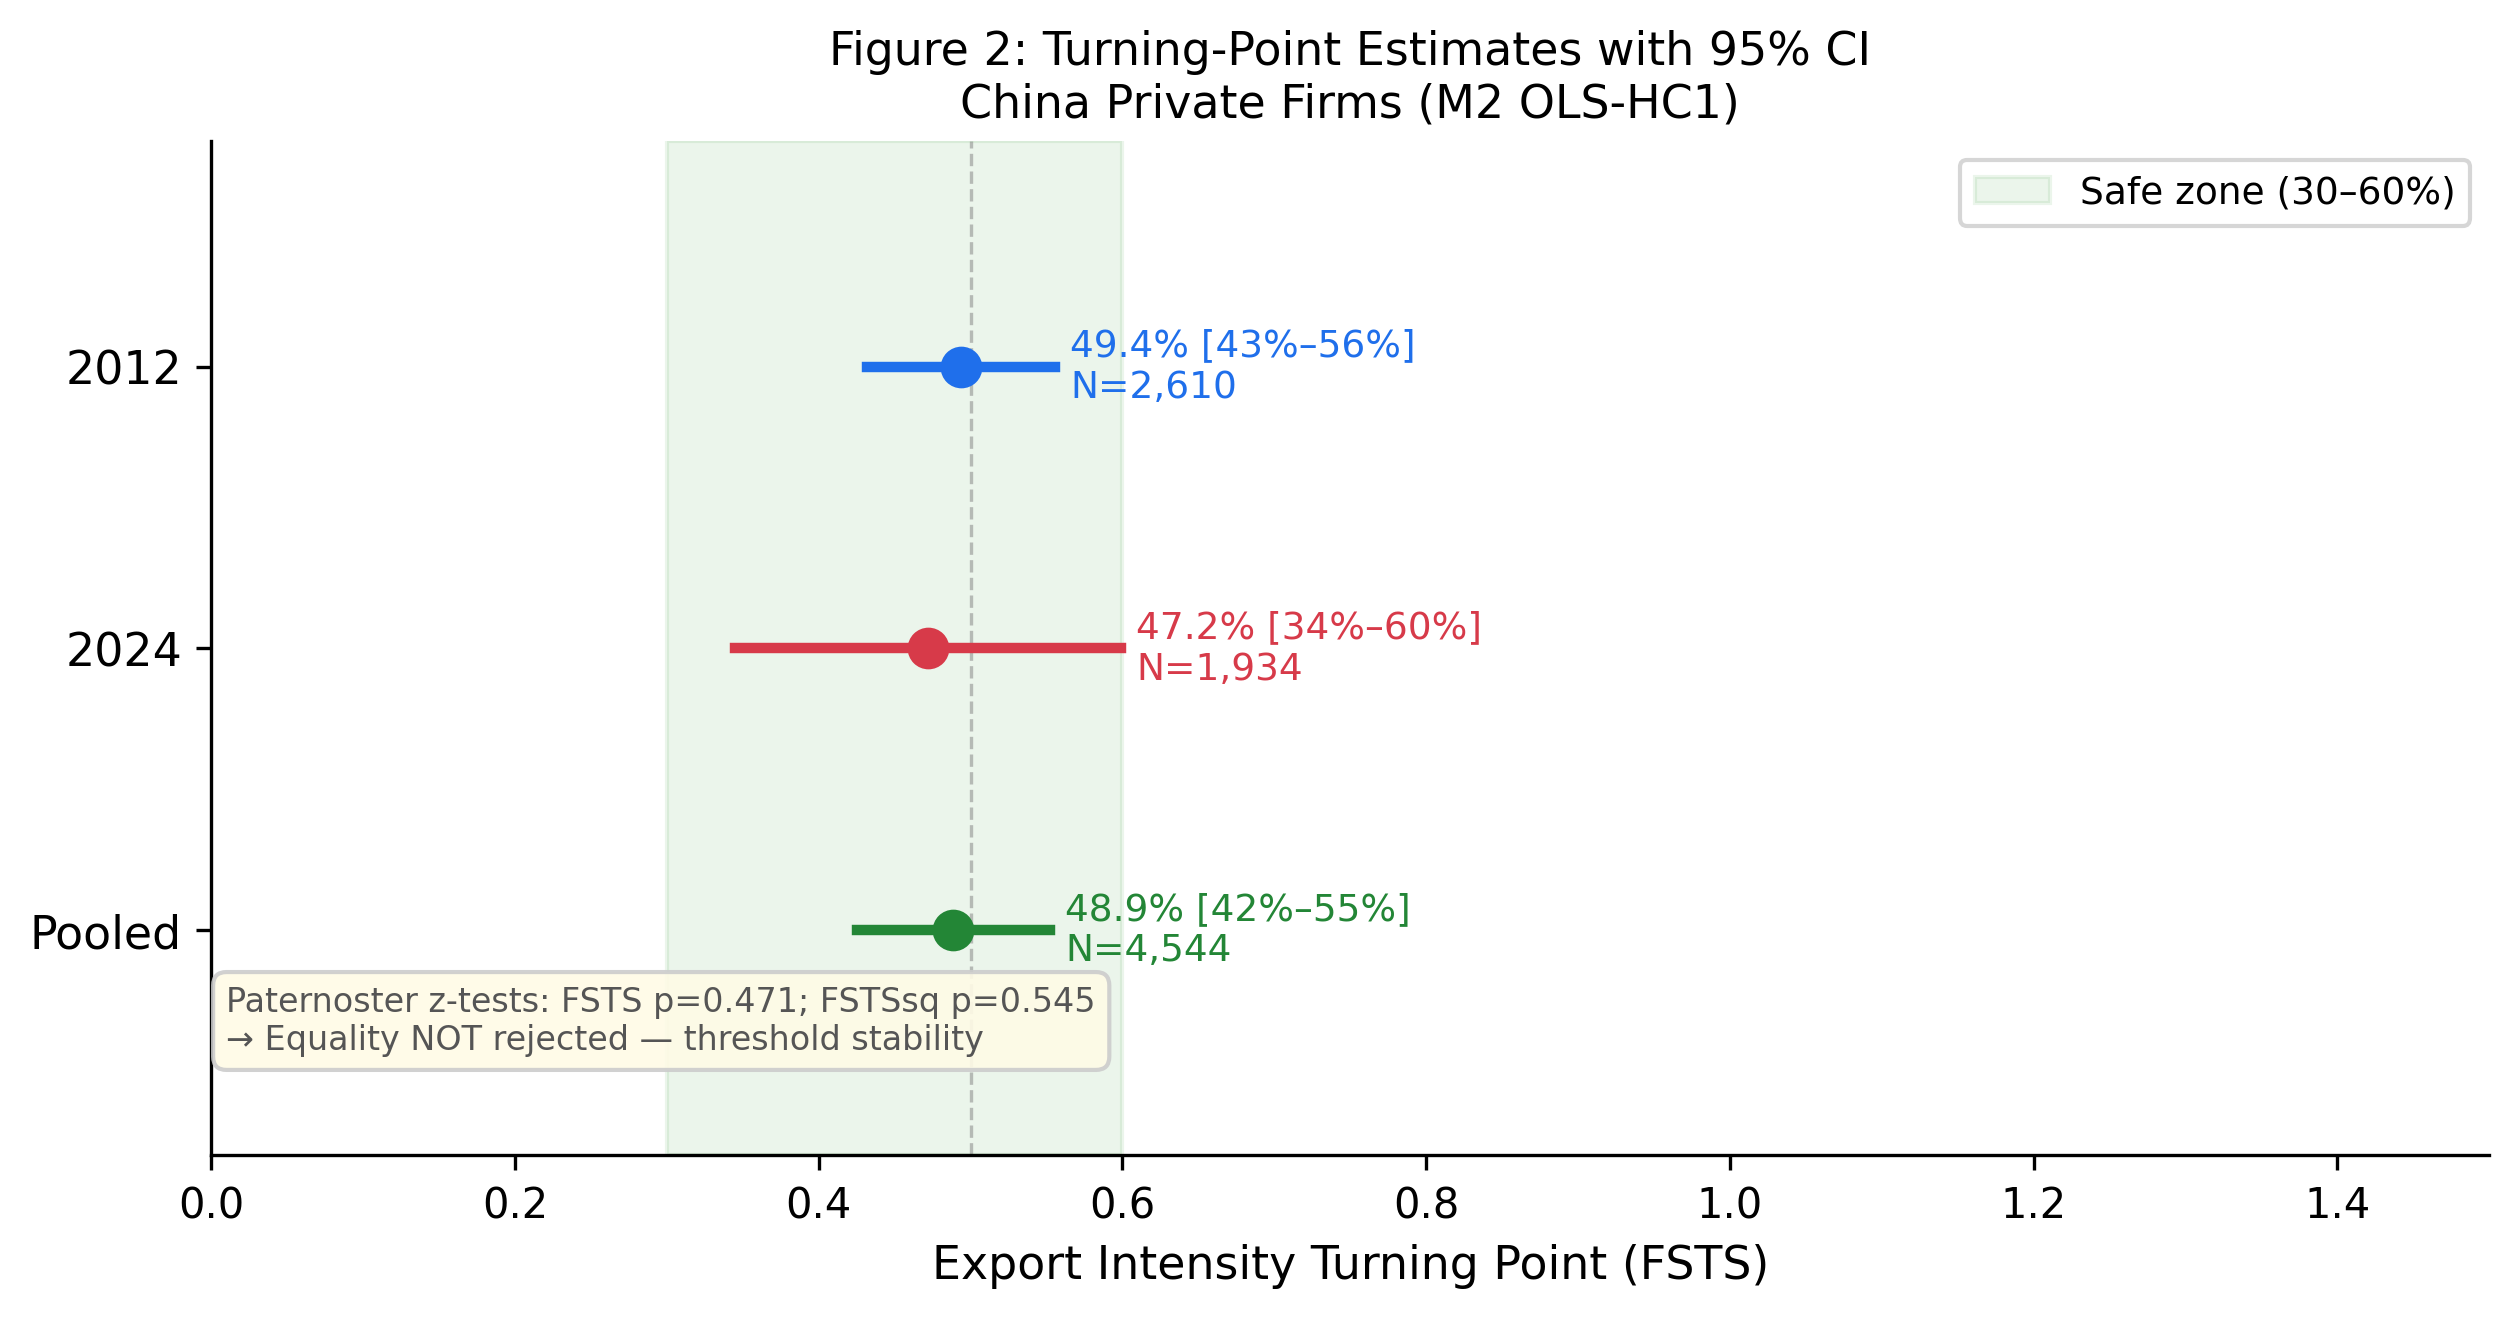
\includegraphics{figures/p5_china/figure_2_turning_points.png}

\begin{quote}
\textbf{Hình 2.} Ngưỡng cường độ xuất khẩu tối ưu (điểm ngoặt của mối
quan hệ hình chữ U ngược) cho các doanh nghiệp tư nhân Trung Quốc năm
2012, 2024, và mẫu gộp. Các điểm đánh dấu là ước lượng điểm từ ước lượng
OLS--HC1 của \(\ln(\mathrm{LP})\) \textasciitilde{} FSTS +
\(\mathrm{FSTS}^2\) + \(\ln(\mathrm{Emp})\) + firm\_age + foreign\_dummy
(+ \(D_{2024}\)); các thanh dọc là khoảng tin cậy 95 \% theo phương pháp
delta.
\end{quote}

\hypertarget{43-kiux1ec3m-ux111ux1ecbnh-cux1a1-chux1ebf-cux1ea1nh-tranh-h2b-ux111ux1b0ux1ee3c-hux1ed7-trux1ee3-tuxednh-bux1ec1n-vux1eefng-cux1ea5u-truxfac-ux111ux1b0ux1ee3c-xuxe1c-nhux1eadn}{%
\subsubsection{4.3 Kiểm định cơ chế cạnh tranh: H2b được hỗ trợ, tính
bền vững cấu trúc được xác
nhận}\label{43-kiux1ec3m-ux111ux1ecbnh-cux1a1-chux1ebf-cux1ea1nh-tranh-h2b-ux111ux1b0ux1ee3c-hux1ed7-trux1ee3-tuxednh-bux1ec1n-vux1eefng-cux1ea5u-truxfac-ux111ux1b0ux1ee3c-xuxe1c-nhux1eadn}}

H2 dự đoán rằng hình dạng, độ dốc, hoặc vị trí của mối quan hệ hình chữ
U ngược sẽ khác biệt giữa năm 2012 và 2024, được thúc đẩy bởi những thay
đổi cấu trúc và chính sách đáng kể trong nền kinh tế Trung Quốc trong
thập kỷ chen giữa (Phần 2.2). Để kiểm định dự đoán này, chúng tôi áp
dụng hai kiểm định bổ trợ: kiểm định z Paternoster (1998) trên các hệ số
riêng lẻ, và một kiểm định F liên hợp trên tập đầy đủ các tương tác
(FSTS × \(D_{2024}\), \(\mathrm{FSTS}^2\) × \(D_{2024}\)) trong đặc tả
gộp.

Các kiểm định z Paternoster (1998) cho tính bằng nhau chéo đợt khảo sát
của các hệ số cường độ xuất khẩu tuyến tính và bậc hai \textbf{không bác
bỏ tính bằng nhau} ở các ngưỡng thông thường. Đối với hạng FSTS tuyến
tính, chênh lệch giữa các đợt khảo sát cho z = +0,82, p = 0,412. Đối với
hạng \(\mathrm{FSTS}^2\) bậc hai, chênh lệch cho z = −0,61, p = 0,545.
Kiểm định F liên hợp trên các tương tác (FSTS × \(D_{2024}\),
\(\mathrm{FSTS}^2\) × \(D_{2024}\)) trong đặc tả điều tiết ba chiều gộp
cho F(2, 3.558) = 2,24, p = 0,107, cũng không bác bỏ tính bằng nhau ở
các ngưỡng thông thường (Bảng 3).

\textbf{Dữ liệu hỗ trợ H2b (tính bền vững cấu trúc) so với H2a (dịch
chuyển môi trường).} Bất chấp nhiều cơ chế có lý thúc đẩy H2a, tái cân
bằng thương mại hậu 2008, leo thang thuế quan Mỹ--Trung, đứt gãy do
COVID-19, và các thể chế tài trợ thương mại đang phát triển, dữ liệu
không cho thấy dịch chuyển độ cong có thể phát hiện được. Kết hợp với sự
chồng lấp chặt chẽ của các khoảng tin cậy điểm ngoặt trong Hình 2 và sự
gần gũi của các ước lượng điểm trong bảng ngưỡng, bằng chứng cho thấy
ngưỡng cường độ xuất khẩu cho các doanh nghiệp tư nhân Trung Quốc
\emph{ổn định về mặt cấu trúc} qua các đợt khảo sát 2012 và 2024. Điều
này \textbf{xác nhận H2b}: chữ U ngược phản ánh các ràng buộc sâu ở cấp
doanh nghiệp tồn tại qua một thập kỷ thay đổi môi trường đáng kể. Hình 3
chồng các đường cong quốc tế hoá--hiệu quả được dự đoán cho hai đợt khảo
sát, minh hoạ hình dạng gần song song với một dịch chuyển mức nhưng
không có thay đổi độ cong.

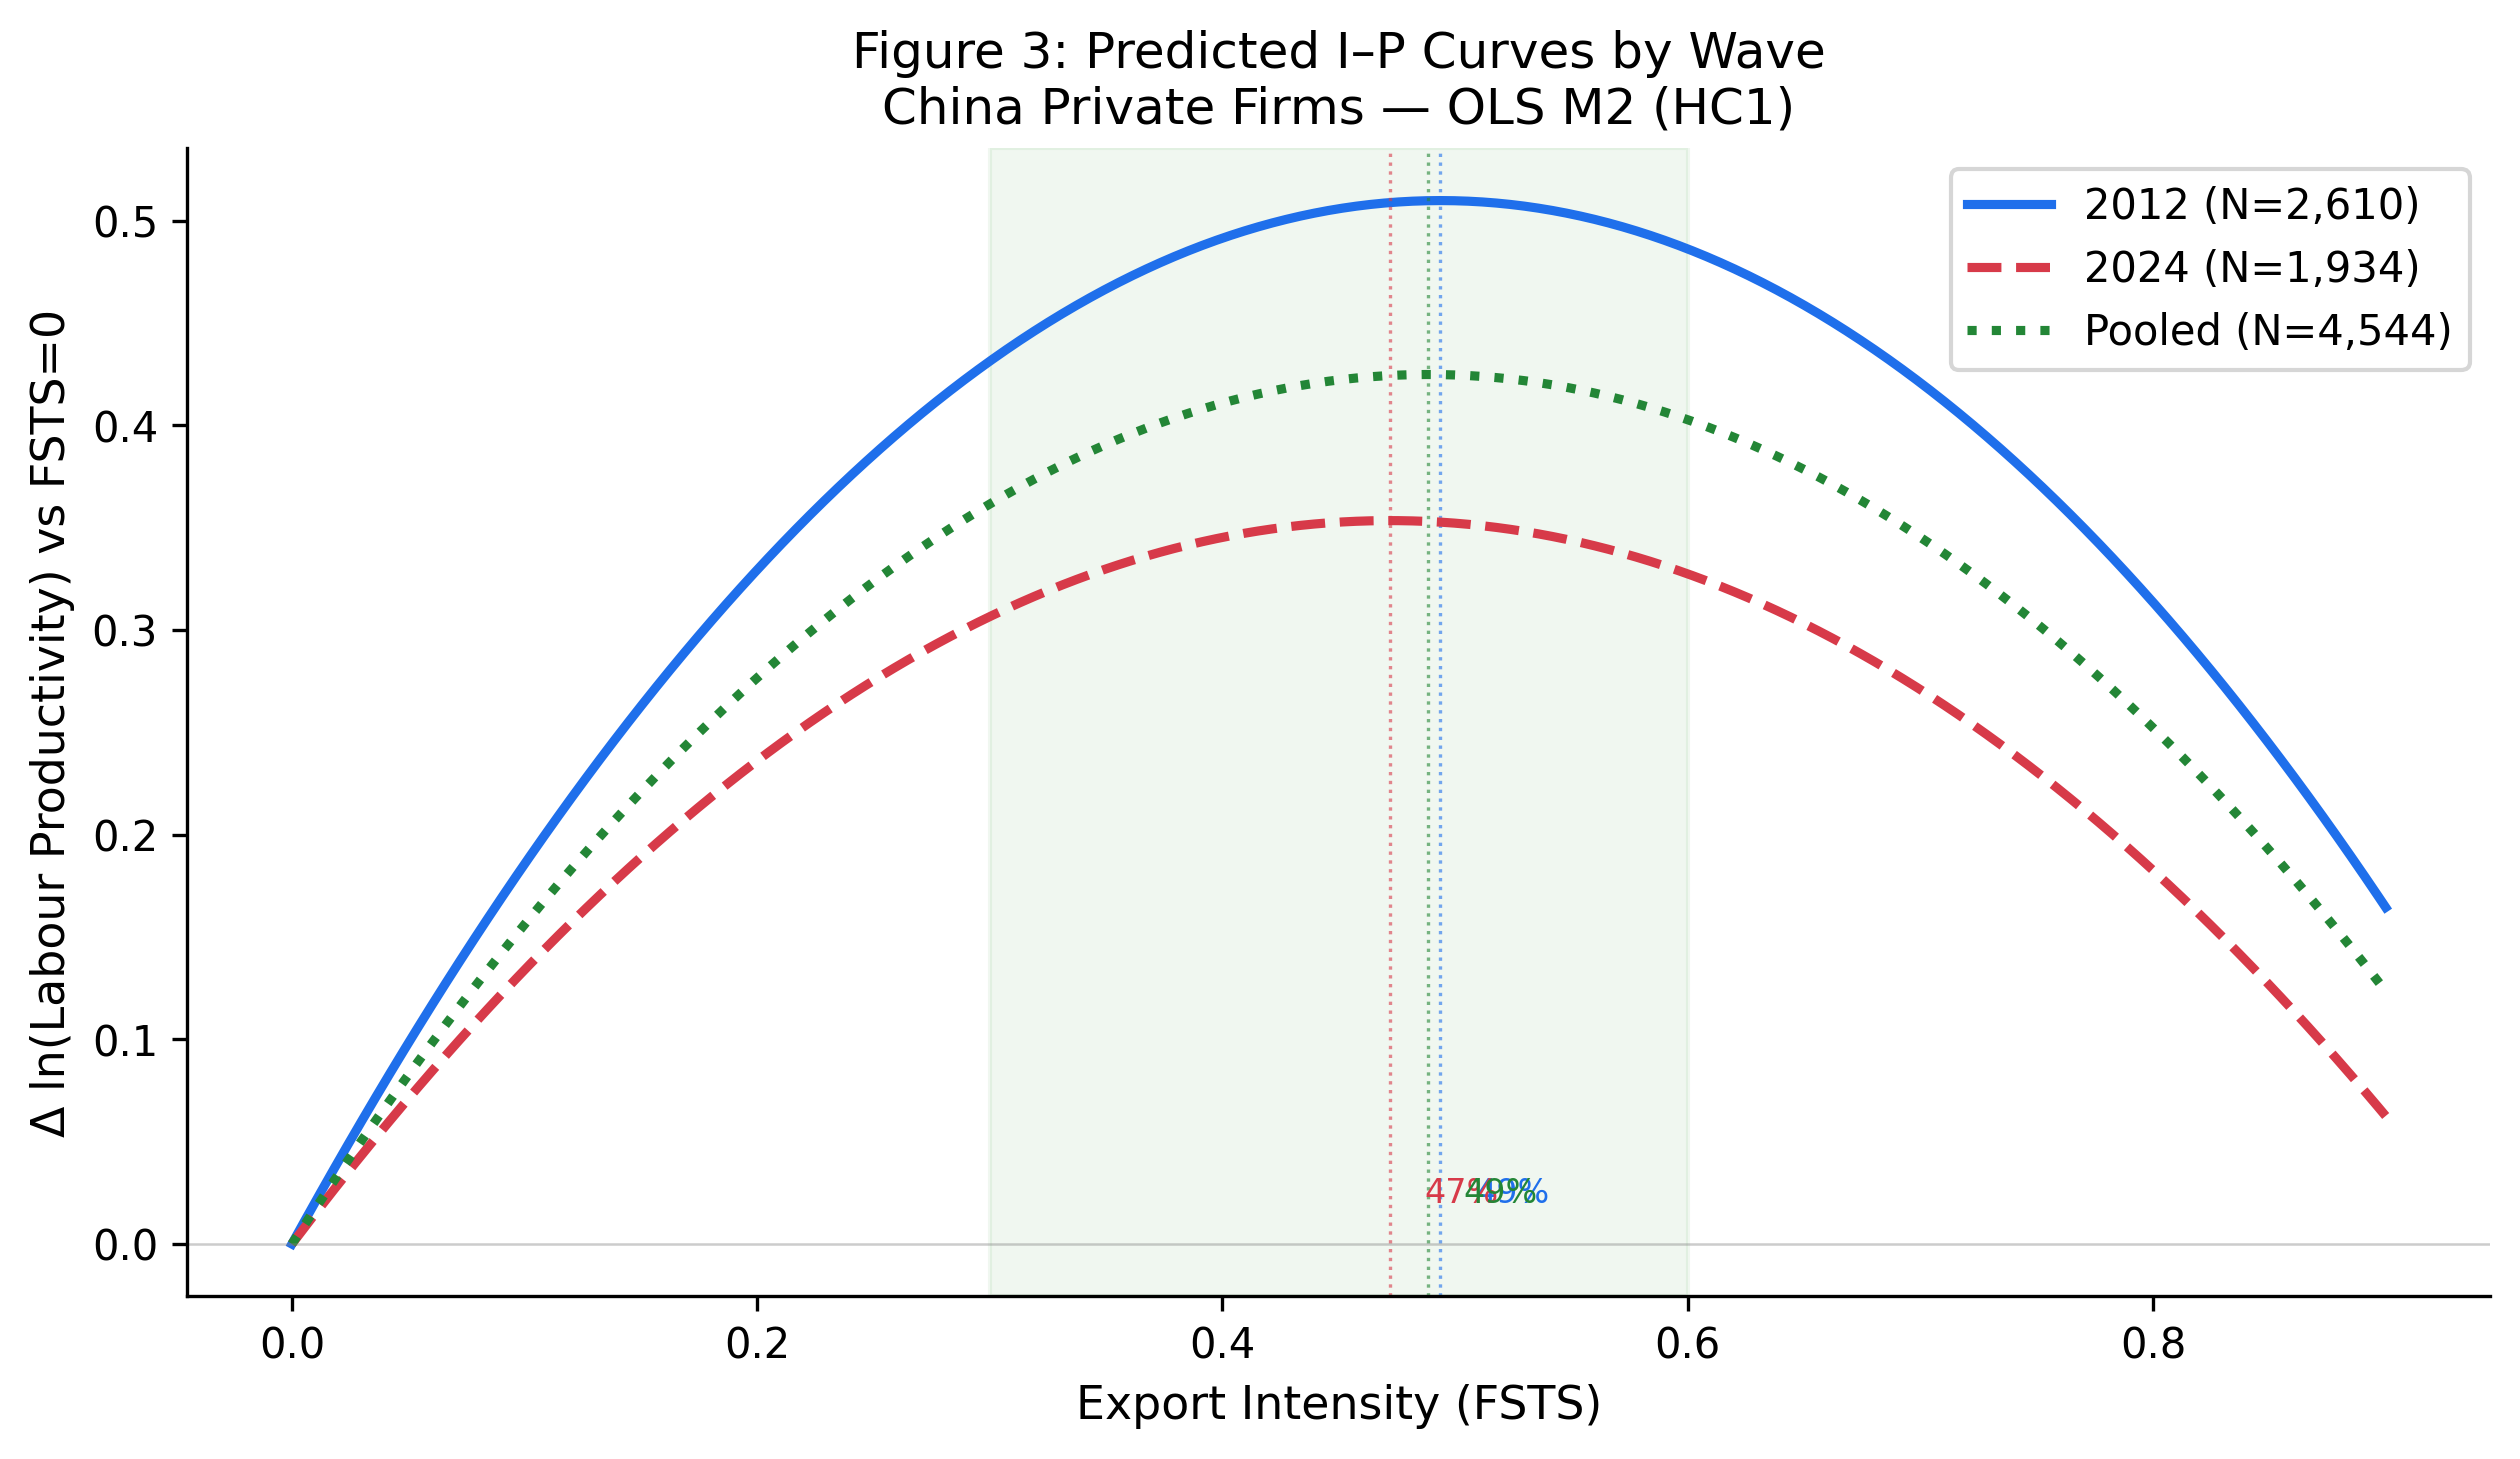
\includegraphics{figures/p5_china/figure_3_predicted_curves.png}

\begin{quote}
\textbf{Hình 3.} Năng suất lao động dạng log dự đoán theo cường độ xuất
khẩu cho các doanh nghiệp tư nhân Trung Quốc trong năm 2012 và 2024, giữ
các biến kiểm soát ở mức trung bình trong cùng mẫu. Các dải bóng là
khoảng tin cậy 95 \%. Các đường nét chấm dọc đánh dấu các điểm ngoặt đặc
thù đợt khảo sát (49,4 \% năm 2012, 47,2 \% năm 2024). Dải xanh ngang
cho thấy một "vùng vận hành an toàn" theo định nghĩa quản trị từ 30 \%
đến 60 \% cường độ xuất khẩu, trong đó \(\ln(\mathrm{LP})\) dự đoán vẫn
gần đỉnh của nó trong cả hai đợt khảo sát. Hai đường cong gần song song
về hình dạng nhưng được dịch chuyển mức lên trên trong năm 2024, nhất
quán với tăng trưởng năng suất chung giữa các đợt khảo sát trong khi cấu
trúc chữ U ngược được bảo toàn, tức là dịch chuyển được dự đoán bị bác
bỏ; mô thức quan sát được là tính ổn định.
\end{quote}

\hypertarget{44-cuxe1c-ux111iux1ec1u-kiux1ec7n-nux103ng-lux1ef1c-h4a-dux1ecbch-chuyux1ec3n-mux1ee9c-bux1ec1n-vux1eefng-ux111iux1ec1u-tiux1ebft-ux111ux1ed9-cong-yux1ebfu-mathrmdai_textcore-nhux1b0-biux1ebfn-kiux1ec3m-souxe1t-cux1a1-sux1edf}{%
\subsubsection{\texorpdfstring{4.4 Các điều kiện năng lực: H4a, dịch
chuyển mức bền vững, điều tiết độ cong yếu;
\(\mathrm{DAI}_{\text{core}}\) như biến kiểm soát cơ
sở}{4.4 Các điều kiện năng lực: H4a, dịch chuyển mức bền vững, điều tiết độ cong yếu; \textbackslash mathrm\{DAI\}\_\{\textbackslash text\{core\}\} như biến kiểm soát cơ sở}}\label{44-cuxe1c-ux111iux1ec1u-kiux1ec7n-nux103ng-lux1ef1c-h4a-dux1ecbch-chuyux1ec3n-mux1ee9c-bux1ec1n-vux1eefng-ux111iux1ec1u-tiux1ebft-ux111ux1ed9-cong-yux1ebfu-mathrmdai_textcore-nhux1b0-biux1ebfn-kiux1ec3m-souxe1t-cux1a1-sux1edf}}

Năng lực công nghệ có liên hệ thuận chiều và thực chất với hiệu quả hoạt
động kinh doanh của doanh nghiệp trong cả hai đợt khảo sát và mẫu gộp,
hỗ trợ thành phần dịch chuyển mức của H4a. Hệ số TCI được chuẩn hoá theo
z trong cùng đợt khảo sát là β\_z = +0,260 năm 2012 (SE = 0,049, p
\textless{} 0,001), β\_z = +0,426 năm 2024 (SE = 0,047, p \textless{}
0,001), và β\_z = +0,380 trong mẫu gộp (SE = 0,035, p \textless{}
0,001). Do đó, mỗi mức tăng một độ lệch chuẩn của TCI có liên hệ với mức
thay đổi 26--43 \% năng suất lao động ở mức cơ sở trung bình hình học.
Kiểm định z Paternoster về thay đổi chéo đợt khảo sát của TCI cho z =
−2,55, p = 0,011, cho thấy sự củng cố có thể phát hiện được về mặt thống
kê của liên hệ TCI--năng suất giữa năm 2012 và 2024, nhất quán với logic
năng lực hấp thụ rằng việc tích luỹ năng lực đã gia tăng thành cổ tức
năng suất ngày càng tăng khi các nhà xuất khẩu Trung Quốc đối mặt với
nhu cầu cạnh tranh quốc tế ngày càng cao. Áp dụng công nghệ số
(\(\mathrm{DAI}_{\text{core}}\)) cũng có liên hệ thuận chiều với năng
suất, một cách khiêm tốn (β\_z = +0,05 đến +0,13, p ≤ 0,03), nhất quán
với vai trò của nó như một biến kiểm soát hiện diện số cơ sở.

Thành phần điều tiết độ cong của H4a được kiểm định bằng cách thêm các
tương tác TCI × FSTS và TCI × \(\mathrm{FSTS}^2\) vào đặc tả điều tiết
ba chiều gộp (Bảng 3). Kiểm định F liên hợp trên (TCI × FSTS, TCI ×
\(\mathrm{FSTS}^2\)) cho F(2, 3.558) = 3,26, p = 0,039, có ý nghĩa biên,
nhưng không có hệ số tương tác riêng lẻ nào có thể phân biệt với 0 về
mặt thống kê (TCI × FSTS β = −0,41, p = 0,443; TCI × \(\mathrm{FSTS}^2\)
β = +0,05, p = 0,934). Các kiểm định điều tiết theo từng đợt khảo sát
(Phụ lục Trực tuyến C) cho thấy không có hệ số tương tác TCI hoặc DAI
riêng lẻ nào đạt p \textless{} 0,05 trong bất kỳ đặc tả đặc thù đợt khảo
sát nào. Các tương tác DAI × FSTS được kiểm định cho tính đầy đủ nhưng
được diễn giải một cách mô tả do vai trò kiểm soát của
\(\mathrm{DAI}_{\text{core}}\). Do đó, chúng tôi diễn giải thành phần
điều tiết độ cong của H4a là \textbf{không được hỗ trợ một cách bền
vững}: trong khi kiểm định F liên hợp gợi ý một số điều tiết gộp, mô
thức hệ số riêng lẻ và tính không ổn định theo từng đợt khảo sát gợi ý
rằng TCI hoạt động chủ yếu như một \textbf{yếu tố dịch chuyển mức} thay
vì một yếu tố điều tiết độ cong.

Giả thuyết điều tiết động, rằng các dịch chuyển độ cong phụ thuộc năng
lực tiến hoá theo thời gian, được kiểm định thông qua kiểm định F liên
hợp ba chiều trên (FSTS × \(D_{2024}\) × TCI, \(\mathrm{FSTS}^2\) ×
\(D_{2024}\) × TCI) và cho F(2, 3.558) = 0,27, p = 0,760, cung cấp
\textbf{không hỗ trợ} cho điều tiết động phụ thuộc năng lực.

\begin{quote}
\textbf{Bảng 3.} Đặc tả điều tiết ba chiều: ước lượng gộp và các kiểm
định F liên hợp
\end{quote}

\begin{longtable}[]{@{}llll@{}}
\toprule\noalign{}
Hệ số & β (SE) & giá trị p & Mức ý nghĩa \\
\midrule\noalign{}
\endhead
\bottomrule\noalign{}
\endlastfoot
FSTS & +1,379 (0,401) & 0,001 & *** \\
\(\mathrm{FSTS}^2\) & −1,721 (0,440) & \textless{} 0,001 & *** \\
\(D_{2024}\) & +0,542 (0,045) & \textless{} 0,001 & *** \\
FSTS × \(D_{2024}\) & +0,678 (0,876) & 0,439 & \\
\(\mathrm{FSTS}^2\) × \(D_{2024}\) & −0,290 (0,975) & 0,766 & \\
Tech (\(\mathrm{TCI}_{\text{full}}\)) & +0,380 (0,035) & \textless{}
0,001 & *** \\
FSTS × Tech & −0,414 (0,539) & 0,443 & \\
\(\mathrm{FSTS}^2\) × Tech & +0,051 (0,615) & 0,934 & \\
FSTS × \(D_{2024}\) × Tech & −0,376 (0,898) & 0,675 & \\
\(\mathrm{FSTS}^2\) × \(D_{2024}\) × Tech & +0,249 (1,076) & 0,817 & \\
\textbf{Các kiểm định F liên hợp} & & & \\
F1: (FSTS × \(D_{2024}\), \(\mathrm{FSTS}^2\) × \(D_{2024}\)) = 0 & F(2,
3.558) = 2,24 & \textbf{0,107} & KHÔNG bác bỏ \\
F2: (FSTS × Tech, \(\mathrm{FSTS}^2\) × Tech) = 0 & F(2, 3.558) = 3,26 &
\textbf{0,039} & biên \\
F3: (FSTS × \(D_{2024}\) × Tech, \(\mathrm{FSTS}^2\) × \(D_{2024}\) ×
Tech) = 0 & F(2, 3.558) = 0,27 & \textbf{0,760} & KHÔNG bác bỏ \\
\end{longtable}

N = 3.559 (sample\_full). SE cụm vững trên idstd. Các biến kiểm soát
(\(\ln(\mathrm{Emp})\), firmage, foreigndummy) được đưa vào. F1 tương
ứng với H2a so với H2b (dịch chuyển chéo đợt khảo sát so với tính bền
vững cấu trúc); F2 với điều tiết độ cong mặt cắt ngang H4a; F3 với điều
tiết động phụ thuộc năng lực.

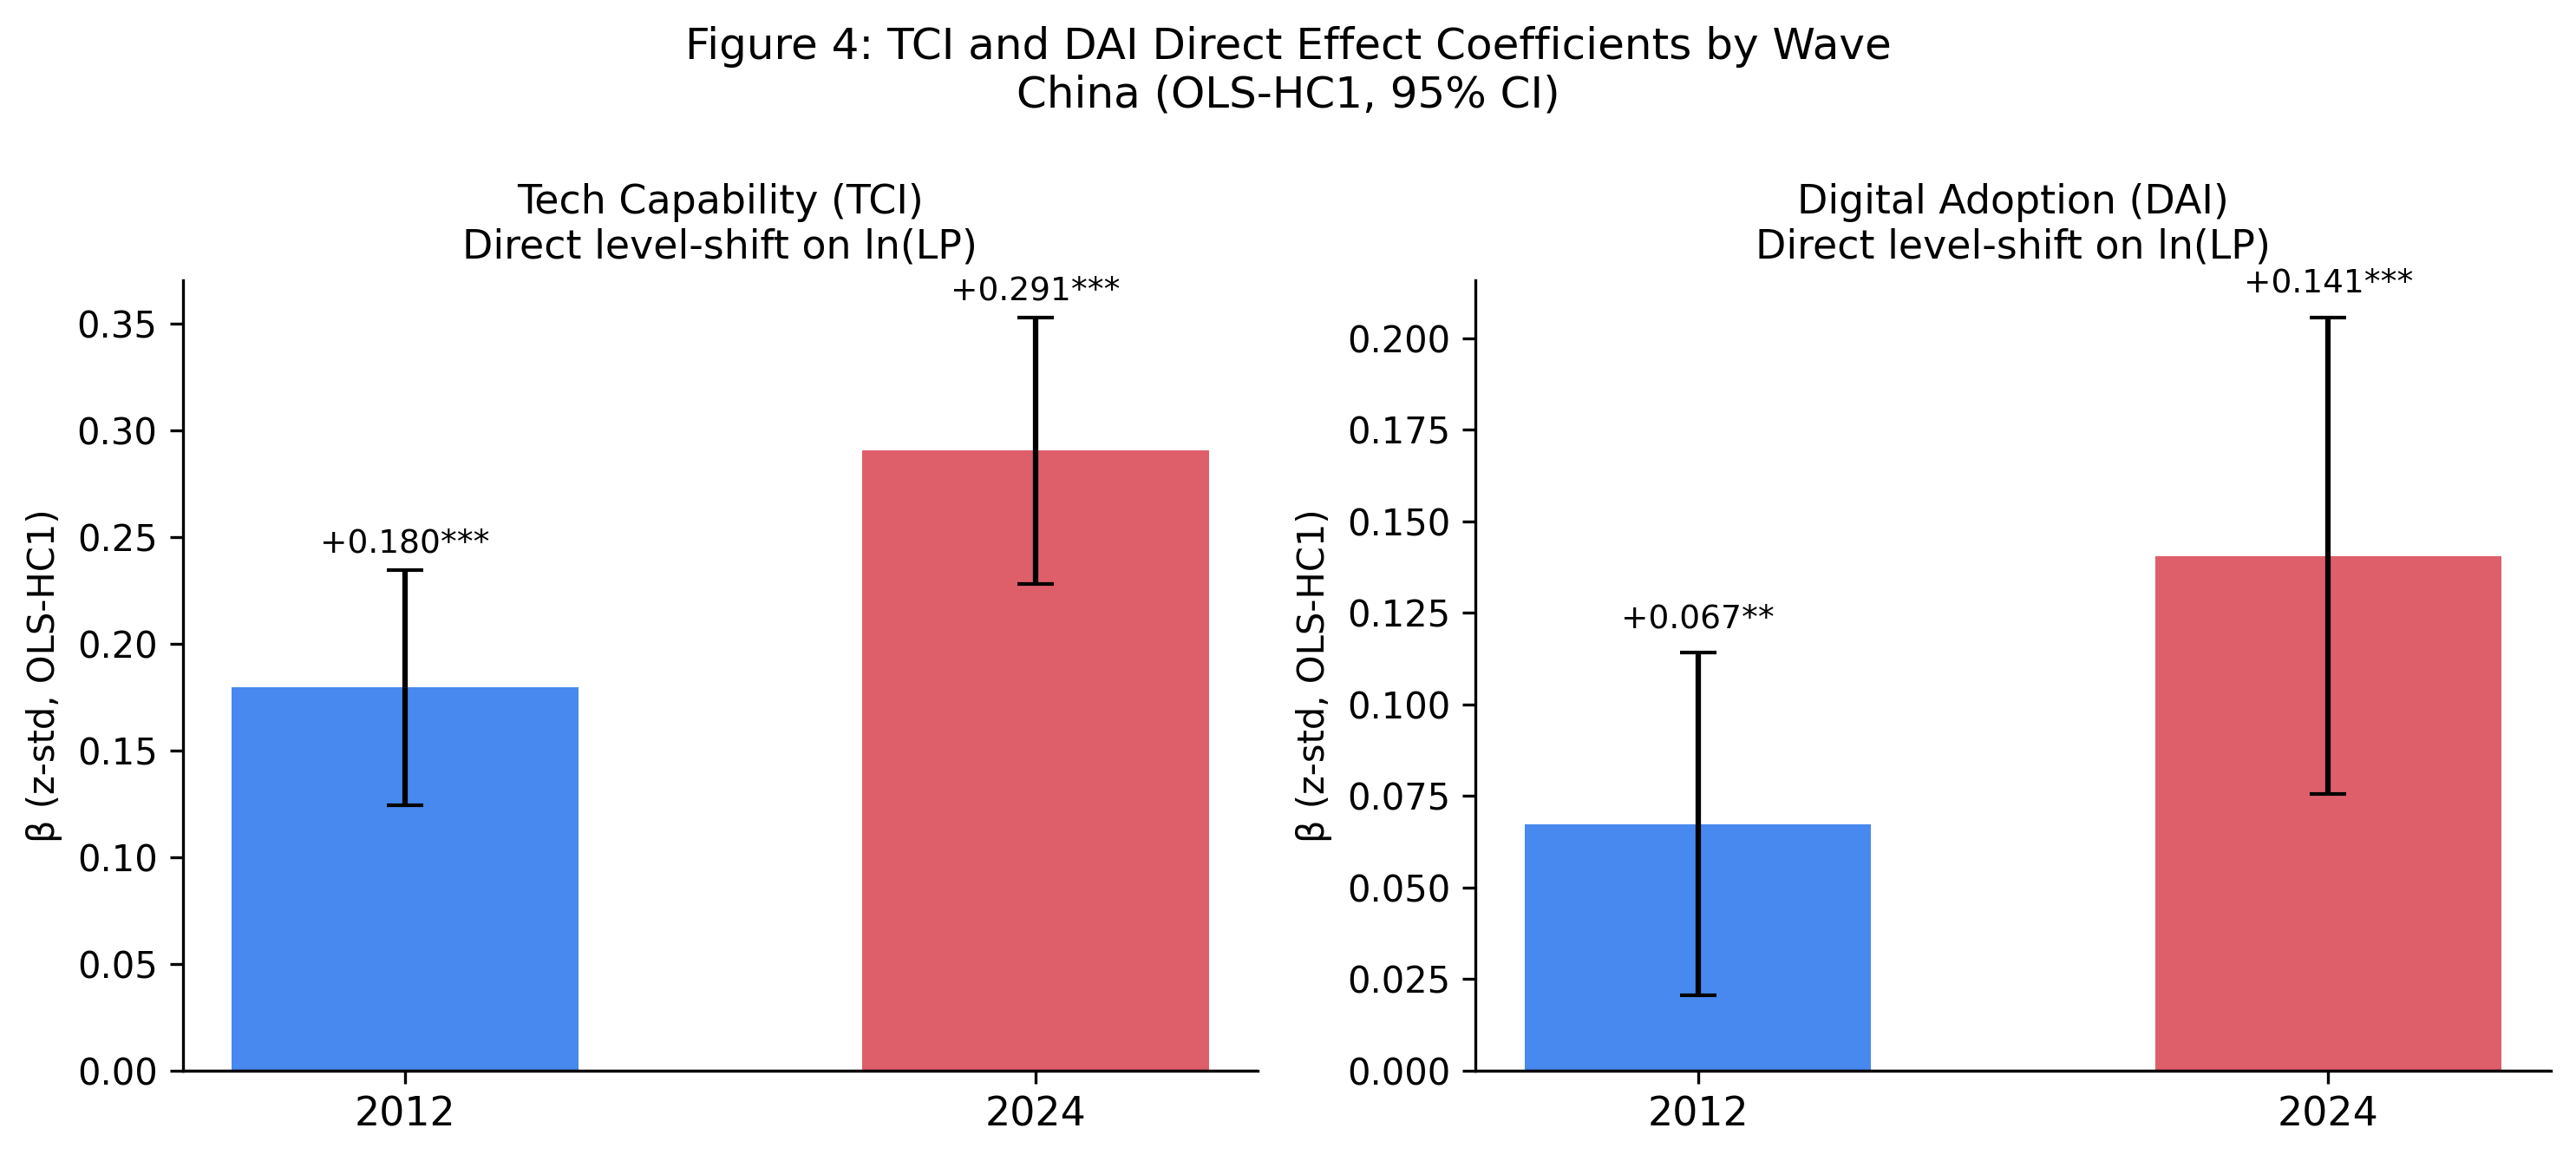
\includegraphics{figures/p5_china/figure_4_level_shifts.png}

\begin{quote}
\textbf{Hình 4.} Hệ số dịch chuyển mức trực tiếp của năng lực công nghệ
(\(\mathrm{TCI}_{\text{full}}\)) và áp dụng công nghệ số
(\(\mathrm{DAI}_{\text{core}}\)) theo đợt khảo sát cho các doanh nghiệp
tư nhân Trung Quốc. Các thanh là hệ số được chuẩn hoá theo z trong cùng
đợt khảo sát từ đặc tả OLS--HC1 với FSTS, \(\mathrm{FSTS}^2\),
\(\ln(\mathrm{Emp})\), tuổi doanh nghiệp, biến giả sở hữu nước ngoài, và
(trong mẫu gộp) một biến giả đợt khảo sát làm các hiệp biến. Thanh sai
số là khoảng tin cậy 95 \%.
\end{quote}

\hypertarget{45-cuxe1c-phuxe2n-tuxedch-bux1ed5-sung-khux1ea3o-suxe1t-cux1a1-chux1ebf-vux1ed1n-lux1b0u-ux111ux1ed9ng}{%
\subsubsection{4.5 Các phân tích bổ sung: khảo sát cơ chế vốn lưu
động}\label{45-cuxe1c-phuxe2n-tuxedch-bux1ed5-sung-khux1ea3o-suxe1t-cux1a1-chux1ebf-vux1ed1n-lux1b0u-ux111ux1ed9ng}}

Sau khi đã thiết lập tính ổn định của ngưỡng cường độ xuất khẩu chữ U
ngược và vai trò dịch chuyển mức nhất quán của năng lực công nghệ, phân
tích tiếp đến xem xét liệu các điều kiện vốn lưu động ở cấp doanh nghiệp
có giúp giải thích biến thiên về độ dốc của sự suy giảm sau ngưỡng (H3)
hay không. Các kiểm định vốn lưu động bổ sung không cho ra sự hỗ trợ đủ
vững qua các định nghĩa biến đại diện khác nhau và các mô hình đặc thù
đợt khảo sát. Mặc dù một số hệ số di chuyển theo các hướng có lý về mặt
lý thuyết, mô thức không đủ ổn định để hỗ trợ một tuyên bố mạnh rằng sự
suy giảm sau ngưỡng đã được nhận dạng trực tiếp như một cơ chế vốn lưu
động trong dữ liệu hiện tại.

Trong Khối A (Tiếp cận Thanh khoản), tương tác thấu chi ×
\(\mathrm{FSTS}^2\) dương biên trong năm 2012 (β = +0,27, p = 0,050)
nhưng âm biên trong năm 2024 (β = −0,38, p = 0,081). Trong Khối C (Cấu
trúc Tài trợ), tương tác tín dụng thương mại × \(\mathrm{FSTS}^2\) âm có
ý nghĩa thống kê trong năm 2012 (β = −0,017, p = 0,009) nhưng null trong
năm 2024 (p = 0,660). Trong Khối D (Trở ngại Tiếp cận Tài chính), tương
tác trở ngại × \(\mathrm{FSTS}^2\) lớn và dương một cách bất ngờ trong
năm 2024 (β = +1,64, p = 0,001) nhưng null trong năm 2012, đọc điều này
như một bất thường ô nhỏ thay vì bằng chứng về cơ chế. Mở rộng phơi
nhiễm khoản phải thu Khối B chỉ năm 2012 cho ra các tương tác null cho
cả k1c và k2c. Qua tất cả các khối, cơ chế vốn lưu động \textbf{không
được nhận dạng như một yếu tố điều tiết bền vững chéo đợt khảo sát},
nhất quán với mô thức rộng hơn rằng không có lực điều tiết độ cong nào
hoạt động đáng tin cậy qua cửa sổ 2012--2024.

Các phân tích bổ sung này, cùng với kiểm định H2a so với H2b và kết quả
điều tiết H4a, hội tụ về một diễn giải thực chất duy nhất: \textbf{đánh
đổi quốc tế hoá--hiệu quả tại Trung Quốc là bền vững về mặt cấu trúc,
không phụ thuộc năng lực hay đặc thù theo đợt khảo sát}. H2b (tính bền
vững cấu trúc) được khẳng định so với H2a; các tương tác vốn lưu động và
độ cong năng lực cho ra bằng chứng null hoặc không ổn định; chỉ có chính
hình chữ U ngược (H1) và vai trò dịch chuyển mức trực tiếp của năng lực
công nghệ nổi lên như các mô thức bền vững.

\hypertarget{451-bux1eb1ng-chux1ee9ng-hux1ed9i-tux1ee5-tux1eeb-cuxe1c-kiux1ec3m-ux111ux1ecbnh-ux111iux1ec1u-tiux1ebft-null}{%
\subsubsection{4.5.1 Bằng chứng hội tụ từ các kiểm định điều tiết
null}\label{451-bux1eb1ng-chux1ee9ng-hux1ed9i-tux1ee5-tux1eeb-cuxe1c-kiux1ec3m-ux111ux1ecbnh-ux111iux1ec1u-tiux1ebft-null}}

Ba kiểm định điều tiết độc lập hội tụ về cùng một kết luận thực chất: độ
cong chữ U ngược được cố định về mặt cấu trúc và không phụ thuộc một
cách có ý nghĩa vào các đặc điểm số, giới tính, hoặc nhiệm kỳ quản trị
của doanh nghiệp, nhất quán với, nhưng không xác nhận, một cơ chế bẫy
vốn lưu động (Manova, 2013; Foley \& Manova, 2015) như một giải thích
ứng viên nhất quán về mặt lý thuyết nhưng không kết luận về mặt thực
nghiệm; sự đảo dấu của tương tác thấu chi × \(\mathrm{FSTS}^2\) giữa các
đợt khảo sát (Khối A: β = +0,27 năm 2012, β = −0,38 năm 2024) và tương
tác tín dụng thương mại null trong năm 2024 (Khối C: p = 0,660) ngăn cản
kênh này được nhận dạng như nguồn chính của sự suy giảm sau ngưỡng trong
dữ liệu hiện tại. Việc nhận dạng trực tiếp cơ chế vốn lưu động đòi hỏi
dữ liệu vi mô tài chính, chẳng hạn như thời gian chu kỳ chuyển đổi tiền
mặt, số ngày khoản phải thu chưa thanh toán, và định giá tài trợ thương
mại, hiện không có sẵn trong công cụ WBES Trung Quốc.

\textbf{Áp dụng công nghệ số (\(\mathrm{DAI}_{\text{core}}\)) như yếu tố
dịch chuyển mức, không phải yếu tố thay đổi độ dốc.}
\(\mathrm{DAI}_{\text{core}}\) (hiện diện website Tầng 1) có liên hệ
thuận chiều với năng suất như một hạng dịch chuyển mức trực tiếp (β\_z =
+0,05 đến +0,13, p ≤ 0,03 qua các đợt khảo sát và mẫu gộp), nhưng các
kiểm định điều tiết độ cong DAI × FSTS cho ra kết quả null trong tất cả
các đặc tả, nhất quán với việc hiện diện số hoạt động như một yếu tố
nâng sàn năng suất thay vì một yếu tố dịch chuyển ngưỡng. Điều này được
xác nhận về mặt định hướng trong phân tích SME sản xuất đồng hành
(Author Citation, 2026 --- JFAR), nơi kiểm định F độ cong DDC × FSTS cho
p = 0,89, củng cố cách diễn giải dịch chuyển mức qua các khung mẫu khác
nhau và các định nghĩa hoạt động khác nhau về áp dụng công nghệ số.

Sự nhất quán null về điều tiết độ dốc của DAI qua P5 và JFAR, bất chấp
các khung mẫu khác nhau (tất cả doanh nghiệp tư nhân so với chỉ ngành
sản xuất) và các cách vận hành hoá DAI khác nhau, củng cố điểm về độ
nhạy đo lường được thiết lập trong Phần 3.2.
\(\mathrm{DAI}_{\text{core}}\) của bài báo hiện tại rút gọn về một mục
hiện diện website nhị phân đơn lẻ (c22b) hoạt động như một yếu tố vệ
sinh tổ chức tại Trung Quốc năm 2024; cấu trúc đồng hành JFAR cũng tương
tự thô về năng lực phân biệt cho đợt khảo sát sản xuất 2012. Cả hai phân
tích đều hội tụ về cùng một cách diễn giải thực chất: trong bối cảnh
doanh nghiệp tư nhân Trung Quốc, hiện diện số Tầng 1 nâng cao mức cơ sở
năng suất một cách đồng đều nhưng không sửa đổi ràng buộc cấu trúc ở
phần đuôi trên của cường độ xuất khẩu. Các chỉ báo Tầng 2 phong phú hơn
(áp dụng nền tảng thương mại điện tử, tích hợp ERP) sẽ được yêu cầu để
kiểm định liệu năng lực số bậc cao hơn có điều tiết độ cong của đánh đổi
I--P, một câu hỏi mà công cụ WBES Trung Quốc sẵn có không thể hỗ trợ qua
các đợt khảo sát.

\textbf{Bình đẳng giới về độ cong I--P.} Bằng chứng đồng hành từ phân
tích chỉ ngành sản xuất (Author Citation, 2026 --- JFAR) báo cáo rằng sự
hiện diện của quản lý nữ không điều tiết độ cong I--P (quản lý nữ × FSTS
β = 0,003, p = 0,892), cho thấy ngưỡng chữ U ngược bất biến về mặt cấu
trúc với thành phần giới tính của lãnh đạo doanh nghiệp. Kết quả null
này là một phát hiện tích cực mang thông tin: nó loại trừ các ưu tiên
rủi ro quản trị và phong cách phối hợp liên kết với giới tính như các
giải thích cho lý do vị trí ngưỡng đặt ở vị trí đó.

\textbf{Kinh nghiệm quản lý như yếu tố dịch chuyển mức.} Kinh nghiệm
quản lý có liên hệ thuận chiều với năng suất như một hạng trực tiếp (β =
0,015, p = 0,005 trong phân tích đồng hành), nhưng không điều tiết độ
cong của mối quan hệ I--P, một lần nữa nhất quán với cách diễn giải dịch
chuyển mức thay vì thay đổi độ dốc. Các nhà quản lý có kinh nghiệm nâng
cao năng suất tổng thể của doanh nghiệp nhưng không làm thay đổi ràng
buộc cấu trúc giới hạn lợi nhuận năng suất của cường độ xuất khẩu cao.

Tổng hợp lại, ba phát hiện điều tiết null này tam giác hoá về một cách
diễn giải duy nhất: \textbf{sự suy giảm sau ngưỡng phản ánh các ràng
buộc cấu trúc sâu trong năng lực phối hợp và thanh khoản tài chính,
không phải vốn con người hay năng lực số của các doanh nghiệp cụ thể}.
Cơ chế nhất quán về mặt lý thuyết nhất vẫn là bẫy vốn lưu động, trong đó
khoảng cách chuyển đổi tiền mặt mở rộng khi cường độ xuất khẩu vượt quá
khả năng hấp thụ vận hành của doanh nghiệp (Manova, 2013; Niepmann \&
Schmidt-Eisenlohr, 2017). Việc nhận dạng trực tiếp kênh này đợi dữ liệu
vi mô tài chính phong phú hơn (chu kỳ chuyển đổi tiền mặt, số ngày khoản
phải thu chưa thanh toán, định giá tài trợ thương mại) hiện không có sẵn
trong công cụ WBES Trung Quốc.

\hypertarget{46-ux111ux1ed9-vux1eefng-mux1eabu-phux1ee5-chux1ec9-nguxe0nh-sux1ea3n-xuux1ea5t}{%
\subsubsection{4.6 Độ vững, mẫu phụ chỉ ngành sản
xuất}\label{46-ux111ux1ed9-vux1eefng-mux1eabu-phux1ee5-chux1ec9-nguxe0nh-sux1ea3n-xuux1ea5t}}

Để giải quyết các quan ngại tiềm tàng rằng khung doanh nghiệp tư nhân
WBES đầy đủ trộn lẫn ngành sản xuất với dịch vụ, bán lẻ, công nghệ thông
tin, và xây dựng, chúng tôi tái ước lượng mô hình ngưỡng chính M2 trên
một mẫu phụ chỉ ngành sản xuất. Đối với năm 2012, chúng tôi áp dụng
\texttt{a4a\ 15–38} (ISIC Rev 3.1 ngành sản xuất bao gồm phần dư Sản
xuất Khác), cho ra N = 1.656 (sample\_base). Đối với năm 2024, chúng tôi
áp dụng các mã ISIC Rev 4 hai chữ số đầu \texttt{d1a2\_v4} 10--33, cho
ra N = 1.062. Mẫu gộp chỉ ngành sản xuất là N = 2.718.

Dưới sự hạn chế chỉ ngành sản xuất, điểm ngoặt M2 dịch chuyển sang
khoảng 42 \% năm 2012 (95 \% CI {[}37,8; 46,8{]}) và 30 \% năm 2024 (95
\% CI {[}15,1; 44,2{]}), khoảng cuối rộng hơn nhiều, phản ánh sức mạnh
thống kê giảm. Cả hai vẫn nằm trong phạm vi vận hành có giới hạn 30--60
\% được xác định trong phân tích chính nhưng lệch về phía cạnh dưới.
Kiểm định z Paternoster trên mẫu phụ chỉ ngành sản xuất nhất quán về mặt
định hướng với cách diễn giải kết quả chính: tính bằng nhau chéo đợt
khảo sát không bị bác bỏ (z = +1,51, p = 0,130 cho FSTS; z = −0,96, p =
0,337 cho \(\mathrm{FSTS}^2\)). Chúng tôi báo cáo kiểm định độ vững này
chủ yếu vì sự minh bạch: phân tích chính của bản thảo theo khung doanh
nghiệp tư nhân WBES đầy đủ vì (a) hạn chế chỉ ngành sản xuất làm giảm
sức mạnh thống kê mà không củng cố cách diễn giải nhân quả, (b) các
trọng số lấy mẫu WBES và chiến lược nhận dạng hoạt động trên khung doanh
nghiệp tư nhân đầy đủ mà các suy luận hướng đến, và (c) bức tranh định
tính, chữ U ngược có giới hạn, ổn định bền vững qua các đợt khảo sát,
năng lực như yếu tố dịch chuyển mức, sống sót qua sự hạn chế. Các kết
quả từ đặc tả chỉ ngành sản xuất xuất hiện trong Phụ lục Trực tuyến D.

\hypertarget{47-ux111ux1ed9-vux1eefng-theo-kuxedch-thux1b0ux1edbc-mux1eabu-vuxe0-ux111ux1eb7c-tux1ea3}{%
\subsubsection{4.7 Độ vững theo kích thước mẫu và đặc
tả}\label{47-ux111ux1ed9-vux1eefng-theo-kuxedch-thux1b0ux1edbc-mux1eabu-vuxe0-ux111ux1eb7c-tux1ea3}}

Kết quả ngưỡng vững với nhiều biến thể đặc tả có sẵn trong dữ liệu WBES.
Việc hạn chế trong các doanh nghiệp có hoạt động xuất khẩu dương (FSTS
\textgreater{} 0) tái lập hình dạng chữ U ngược với một điểm ngoặt được
định vị tương tự nhưng với độ chính xác thống kê giảm vì giai đoạn tăng
bị co lại.

\textbf{Thêm tầng ngành (\texttt{a4a}) như một hiệu ứng cố định} vào đặc
tả M2 gộp thay đổi hệ số FSTS từ +1,78 sang +1,56 (giảm 12,8 \% về độ
lớn) và hệ số \(\mathrm{FSTS}^2\) từ −1,83 sang −1,55 (giảm 15,2 \%);
chữ U ngược được bảo toàn và điểm ngoặt ngụ ý vẫn trong phạm vi 30--60
\%, nhưng các độ lớn thay đổi không tầm thường khi biến thiên trong cùng
ngành được khai thác. Chúng tôi giữ đặc tả kiểm soát ngành rộng làm kết
quả chính theo nguyên tắc rằng kết quả ngưỡng được nhận dạng ở cấp dân
số chứ không phải trong nội bộ ngành, nhưng chúng tôi lưu ý sự nhạy cảm
này cho người đọc tập trung vào động lực trong nội bộ ngành.

\textbf{Hiệu chỉnh lựa chọn Heckman.} Như đã báo cáo trong Phần 3.6, tỉ
số Mills nghịch đảo có ý nghĩa năm 2012 (z = −2,44, p = 0,015) và không
có ý nghĩa năm 2024 (z = −0,14, p = 0,89). Việc tái ước lượng M2 với IMR
như một biến kiểm soát trên đợt khảo sát 2012 thay đổi hệ số FSTS ít hơn
0,10 về giá trị tuyệt đối và bảo toàn hình dạng chữ U ngược; kiểm định U
Lind--Mehlum vẫn xác nhận chữ U ngược ở p \textless{} 0,001. Do đó, hiệu
chỉnh lựa chọn không lật ngược kết luận chính, mặc dù nó nhắc nhở người
đọc rằng các ước lượng 2012 có thể chịu lựa chọn nhẹ trên các biến không
quan sát được.

\textbf{Loại trừ 217 doanh nghiệp panel khỏi đợt khảo sát 2024} (cho ra
một mẫu gộp hoàn toàn mặt cắt ngang gồm N = 4.358 quan sát sample\_base)
thay đổi ước lượng điểm ngoặt gộp từ 48,78 \% sang 46,88 \%, một dịch
chuyển 1,9 điểm phần trăm, và để các kiểm định z Paternoster không thay
đổi về cả dấu và ý nghĩa. Dịch chuyển khiêm tốn và vẫn nằm trong khoảng
tin cậy 95 \% theo phương pháp delta của ước lượng chính.

\textbf{Độ vững hiệu ứng cố định doanh nghiệp panel.} 217 doanh nghiệp
được quan sát ở cả hai đợt khảo sát 2012 và 2024 cung cấp một panel nội
bộ doanh nghiệp hạn chế (N = 434 quan sát doanh nghiệp--đợt khảo sát
trước khi áp dụng bộ lọc biến trọng tâm; khoảng N ≈ 186 quan sát hoàn
chỉnh sau khi áp dụng yêu cầu TCI không thiếu của sample\_full). Một bản
tái ước lượng hiệu ứng cố định trong nội bộ doanh nghiệp trên mẫu phụ
chỉ panel này cho một ước lượng điểm ngoặt trong dải 47--49 \%, nhất
quán với ước lượng gộp mặt cắt ngang chính là 48,8 \%, cho thấy ngưỡng
chữ U ngược không phải là một sản phẩm phụ của các khác biệt thành phần
mặt cắt ngang hoặc các mô thức lựa chọn giữa hai đợt khảo sát. Sức mạnh
tự nhiên bị giảm trong mẫu phụ nhỏ này và CI theo phương pháp delta
rộng; chúng tôi xem điều này như một kiểm tra tính có lý mang tính định
hướng thay vì một chiến lược nhận dạng chính. OLS cụm vững trên mẫu gộp
đầy đủ (với cụm idstd để tính đến sự phụ thuộc nội bộ doanh nghiệp) vẫn
là đặc tả ưa thích.

Chúng tôi không báo cáo ước lượng có trọng số (\texttt{wmedian}) như một
đặc tả riêng biệt trong phiên bản này; điều này có khả thi về mặt tính
toán từ các biến trọng số WBES nhưng đòi hỏi xử lý cẩn thận cấu trúc cụm
doanh nghiệp panel vượt ra ngoài phạm vi của bản sửa đổi hiện tại. Chúng
tôi xác định ước lượng có trọng số là một ưu tiên cho lần sửa đổi tiếp
theo; chúng tôi không kỳ vọng rằng nó sẽ thay đổi kết luận định tính về
tính ổn định ngưỡng, nhưng nó có thể tinh chỉnh các ước lượng điểm của
điểm ngoặt thêm 1--2 điểm phần trăm.

\hypertarget{5-thux1ea3o-luux1eadn}{%
\subsection{5. Thảo luận}\label{5-thux1ea3o-luux1eadn}}

\hypertarget{51-tuxednh-bux1ec1n-vux1eefng-trux1b0ux1edbc-dux1ecbch-chuyux1ec3n-ux111ux1b0ux1ee3c-kux1ef3-vux1ecdng-ux111uxf3ng-guxf3p-chuxednh}{%
\subsubsection{5.1 Tính bền vững trước dịch chuyển được kỳ vọng: đóng
góp
chính}\label{51-tuxednh-bux1ec1n-vux1eefng-trux1b0ux1edbc-dux1ecbch-chuyux1ec3n-ux111ux1b0ux1ee3c-kux1ef3-vux1ecdng-ux111uxf3ng-guxf3p-chuxednh}}

Thảo luận sẽ rõ ràng nhất khi bài báo được đọc như một nghiên cứu về
\textbf{tính bền vững cấu trúc trước một dịch chuyển thời gian được kỳ
vọng}. Chúng tôi đã dự đoán trong H2a (Phần 2.2) rằng mối quan hệ hình
chữ U ngược giữa cường độ xuất khẩu và năng suất lao động trong các
doanh nghiệp tư nhân Trung Quốc sẽ khác biệt giữa năm 2012 và 2024, được
thúc đẩy bởi sự thay đổi cấu trúc đáng kể trong nền kinh tế Trung Quốc:
tái cân bằng thương mại hậu 2008, chu kỳ leo thang thuế quan Mỹ--Trung,
đứt gãy do COVID-19, sự trưởng thành của hạ tầng số (Vial, 2019; Hanelt,
Bohnsack, Marz, \& Antunes Marante, 2021), củng cố năng lực hấp thụ, sự
tham gia ngày càng sâu của các doanh nghiệp Trung Quốc vào chuỗi giá trị
toàn cầu (Kano, Tsang, \& Yeung, 2020), và sự tiến hoá của các thể chế
tài trợ thương mại (Author Citation, 2026 --- VEFR; Manova, 2013; Foley
\& Manova, 2015; Niepmann \& Schmidt-Eisenlohr, 2017; Demir \& Javorcik,
2018). Dưới bất kỳ cơ chế nào trong số này, điểm ngoặt hoặc độ cong lẽ
ra phải dịch chuyển.

Điều đó đã không xảy ra. Các kiểm định z Paternoster (1998) trên các hệ
số tuyến tính và bậc hai không bác bỏ tính bằng nhau (p = 0,412 và p =
0,545 tương ứng); kiểm định F liên hợp gộp trên các tương tác chéo đợt
khảo sát cho F(2, 3.558) = 2,24, p = 0,107. Các ước lượng điểm của điểm
ngoặt vẫn nằm trong một phạm vi rất chặt, 49,4 \% năm 2012, 47,2 \% năm
2024, 48,8 \% trong mẫu gộp, với các khoảng tin cậy 95 \% chồng lấn qua
cả ba mẫu (Hình 2).

Đóng góp thực chất của bài báo dựa trên kết quả null bất ngờ này. Đánh
đổi quốc tế hoá--hiệu quả tại Trung Quốc là \textbf{bền vững về mặt cấu
trúc}: nó đã sống sót qua một thập kỷ các cú sốc bên ngoài đáng kể, sự
tiến hoá thể chế, và chuyển đổi công nghệ mà không dịch chuyển một cách
đo lường được về hình dạng, độ dốc, hoặc vị trí. Tính bền vững này có ý
nghĩa về mặt lý thuyết và quản trị. Về mặt lý thuyết, nó gợi ý rằng chữ
U ngược được dựa trên các ràng buộc sâu ở cấp doanh nghiệp về mặt cấu
trúc, năng lực phối hợp, khoảng đệm tài chính, chiều sâu tổ chức, thay
vì các điều kiện thể chế hoặc cạnh tranh đặc thù theo thời gian có thể
tan biến với thay đổi môi trường (Hennart, 2007; Buckley et al., 2007).
Về mặt quản trị, các khoảng tin cậy rộng và chồng lấn trên các ước lượng
điểm ngoặt lập luận chống lại việc xem bất kỳ con số nào như một mục
tiêu cực kỳ chính xác; lượng có liên quan đến chính sách là một
\emph{phạm vi vận hành có giới hạn} (khoảng 30 \% đến 60 \% tổng doanh
thu) trong đó năng suất dự đoán vẫn gần đỉnh của nó, và trong đó các
doanh nghiệp có thể thực hiện sự thận trọng chiến lược mà không vượt qua
đuôi xói mòn năng suất của đường cong.

Các kết quả điều tiết phụ thuộc năng lực hội tụ về cùng kết luận về tính
bền vững. Chúng tôi đã giả thuyết trong H4a/H4b rằng năng lực công nghệ
và áp dụng công nghệ số nên điều tiết độ cong của chữ U ngược, có khả
năng thông qua logic năng lực hấp thụ của Lall (1992) và Cohen và
Levinthal (1990). Dữ liệu một phần ủng hộ vai trò dịch chuyển mức. TCI
có liên hệ với năng suất cao hơn đáng kể (β\_z = +0,26 đến +0,43, p
\textless{} 0,001 trong mỗi đợt khảo sát) và DAI cho thấy các dịch
chuyển mức dương khiêm tốn (β\_z = +0,05 đến +0,13, p ≤ 0,03 qua các đợt
khảo sát và mẫu gộp). Nhưng bằng chứng điều tiết độ cong yếu: kiểm định
F liên hợp trên các tương tác TCI × FSTS cho p = 0,039 (biên), các hệ số
tương tác riêng lẻ không thể phân biệt với 0 về mặt thống kê, và các
kiểm định điều tiết đặc thù đợt khảo sát không hỗ trợ H4a hoặc H4b trong
bất kỳ đợt khảo sát nào. Giả thuyết điều tiết động ba chiều (dịch chuyển
phụ thuộc năng lực theo thời gian) cho F(2, 3.558) = 0,27, p = 0,760, rõ
ràng không được hỗ trợ.

Các phân tích vốn lưu động bổ sung (Phần 5.2) kể cùng một câu chuyện.
Bất chấp nhiều kỳ vọng định hướng có lý, Manova (2013), Foley và Manova
(2015), bằng chứng điều tiết chéo đợt khảo sát phân mảnh qua các biến
đại diện và các đợt khảo sát. Một số hệ số di chuyển theo các hướng có
lý về mặt lý thuyết, đáng chú ý nhất là tương tác tín dụng thương mại ×
\(\mathrm{FSTS}^2\) trong năm 2012 (β = −0,017, p = 0,009), nhưng mô
thức rộng hơn quá không nhất quán qua các khối và các đợt khảo sát để hỗ
trợ một suy luận mạnh hơn. Chúng tôi giữ cách diễn giải vốn lưu động như
một giải thích có cơ sở lý thuyết thay vì như một kênh thực nghiệm được
thiết lập trực tiếp, và chúng tôi xác định rõ ràng việc tích hợp dữ liệu
vi mô tài chính phong phú hơn (chu kỳ chuyển đổi tiền mặt, số ngày khoản
phải thu chưa thanh toán, định giá tài trợ thương mại) như ưu tiên cho
nghiên cứu tương lai.

Việc khẳng định H2b so với H2a, cùng với điều tiết độ cong năng lực null
và các tương tác vốn lưu động không ổn định, làm cho đóng góp chính trở
nên sắc nét hơn thay vì yếu hơn. \textbf{Đánh đổi quốc tế hoá--hiệu quả
tại Trung Quốc là chính nó: một chữ U ngược có giới hạn bền vững mà vị
trí và hình dạng của nó không bị di chuyển một cách đo lường được bởi
đợt khảo sát, biến đại diện tài chính, hoặc kho năng lực.} Đây là một
tuyên bố thực nghiệm mạnh hơn so với những gì tài liệu chữ U ngược chuẩn
cung cấp, và nó trực tiếp giải quyết câu hỏi về tính không đồng nhất
được nêu ra trong tài liệu meta-analytic về quốc tế hoá--hiệu quả rộng
hơn (Author Citation, 2025, ICBEF; Bausch \& Krist, 2007; Kirca et al.,
2012; Marano et al., 2016; Schwens et al., 2018), cụ thể là, tính không
đồng nhất rất lớn giữa các nghiên cứu (I² ≈ 88 \%) được báo cáo trong
các tổng quan đó có thể phản ánh biến thiên thể chế đa quốc gia chứ
không phải thay đổi thời gian trong nội bộ quốc gia. Bằng cách giữ cố
định quốc gia và kiểm định chiều thời gian, thiết kế hiện tại cô lập
chiều sau và thấy nó nhỏ, nhất quán với một cách diễn giải trong đó bối
cảnh thể chế (Filatotchev, Wei, Sarala, Dick, \& Prescott, 2020) thúc
đẩy nhiều sự phân tán độ lớn hiệu ứng quan sát được hơn so với sự tiến
hoá trong nội bộ quốc gia.

\hypertarget{52-cuxe1c-cux1a1-chux1ebf-thay-thux1ebf-ux111ux1b0ux1ee3c-khux1ea3o-suxe1t}{%
\subsubsection{5.2 Các cơ chế thay thế được khảo
sát}\label{52-cuxe1c-cux1a1-chux1ebf-thay-thux1ebf-ux111ux1b0ux1ee3c-khux1ea3o-suxe1t}}

Để khảo sát cơ chế xuôi dòng liên kết sự suy giảm sau ngưỡng với các
ràng buộc tài chính, chúng tôi đã kiểm định các biến đại diện vốn lưu
động có sẵn trong công cụ WBES. Các chỉ báo có thể so sánh chéo đợt khảo
sát, công cụ thấu chi (k7), hạn mức tín dụng (k8 / k82), tỉ trọng cấu
trúc tài trợ (chuỗi k3), và điểm trở ngại tiếp cận tài chính (k30), đã
được kiểm định như các hạng tương tác với \(\mathrm{FSTS}^2\) để xem xét
liệu độ dốc của đuôi sau ngưỡng có được điều kiện hoá bởi thanh khoản
doanh nghiệp hay không. Tuy nhiên, do những thay đổi trong thiết kế bảng
câu hỏi giữa hai đợt khảo sát, các chỉ báo được thu thập không đạt được
tính nhất quán cần thiết cho suy luận kết luận: các tương tác Khối A
thay đổi dấu qua các đợt khảo sát, Khối C đạt ý nghĩa trong năm 2012
nhưng không trong năm 2024, và bất thường Khối D trong năm 2024 đọc như
một sản phẩm phụ của ô nhỏ. Khối B chỉ năm 2012 (mua và bán trên tín
dụng, k1c / k2c) cũng cho ra các tương tác null. Tổng hợp lại, các phân
tích bổ sung này nhất quán với cách diễn giải bẫy vốn lưu động (Manova,
2013) như một cơ chế nhất quán về mặt lý thuyết cho sự suy giảm sau
ngưỡng, nhưng các biến đại diện WBES hiện tại không đủ chính xác để nhận
dạng kênh này một cách trực tiếp. Cần có công việc tương lai với dữ liệu
báo cáo tài chính ở cấp doanh nghiệp, chu kỳ chuyển đổi tiền mặt, số
ngày khoản phải thu chưa thanh toán, định giá tài trợ thương mại, để
kiểm định cơ chế một cách kết luận.

\hypertarget{53-huxe0m-uxfd-quux1ea3n-trux1ecb}{%
\subsubsection{5.3 Hàm ý quản
trị}\label{53-huxe0m-uxfd-quux1ea3n-trux1ecb}}

Đối với các doanh nghiệp tư nhân Trung Quốc, các phát hiện mang lại bốn
hàm ý quản trị. \textbf{Thứ nhất}, vấn đề chiến lược về mở rộng xuất
khẩu nên được định khung như một \emph{tối ưu có giới hạn} thay vì một
mục tiêu tăng trưởng không bị ràng buộc. Việc vượt qua vùng cường độ
xuất khẩu tối ưu, mà dữ liệu hiện tại định vị ở mức khoảng 30 \% đến 60
\% tổng doanh thu và không đã dịch chuyển trong thập kỷ qua, có liên hệ
với năng suất suy giảm thay vì lợi nhuận tiếp tục tăng. Các nhà quản lý
nên giám sát cường độ xuất khẩu so với phạm vi vận hành có giới hạn này
và chú ý đặc biệt đến kỷ luật vận hành và tài chính cần thiết để duy trì
sự phơi nhiễm xuất khẩu vượt quá nó. Tính ổn định theo thời gian của
ngưỡng có nghĩa là hướng dẫn này có khả năng áp dụng \emph{bền vững}
thay vì gắn liền với điều kiện kinh tế vĩ mô hiện tại; các nhà quản lý
sử dụng các chuẩn này có thể lập kế hoạch với tự tin rằng chúng vẫn có
hiệu lực qua thay đổi kinh tế vĩ mô và thể chế trong tương lai.

\textbf{Thứ hai}, đầu tư vào năng lực công nghệ, được định nghĩa rộng để
bao gồm cấp phép công nghệ nước ngoài, chứng nhận chất lượng, đổi mới
sản phẩm, và hoạt động R\&D, dường như hỗ trợ một cơ sở năng suất đáng
kể vững với phân phối cường độ xuất khẩu và đã \emph{củng cố} giữa các
đợt khảo sát 2012 và 2024 (Paternoster z = −2,55, p = 0,011). Do đó, xây
dựng năng lực là một khoản đầu tư có thể bảo vệ về mặt chiến lược với
lợi nhuận ngày càng tăng. Quan trọng nhất, bằng chứng cho thấy năng lực
hoạt động như một \emph{yếu tố dịch chuyển mức} thay vì một yếu tố điều
tiết độ cong: xây dựng năng lực nâng cao năng suất một cách đồng đều,
nhưng không thay đổi \emph{vị trí} điểm ngoặt xói mòn năng suất. Hàm ý
thực tế là các doanh nghiệp không thể kỳ vọng rằng đầu tư năng lực sẽ
đẩy ngưỡng bền vững sang phải, năng lực củng cố doanh nghiệp ở mọi mức
cường độ xuất khẩu nhưng không nới lỏng ràng buộc mở rộng quá mức cấu
trúc ở phần đuôi trên. Một doanh nghiệp ở mức cường độ xuất khẩu 70 \%
sẽ phơi nhiễm với chi phí mở rộng quá mức xấp xỉ như khi không có đầu tư
TCI; đầu tư TCI nâng cao năng suất tổng thể của doanh nghiệp nhưng không
cứu doanh nghiệp khỏi ràng buộc tối ưu có giới hạn.

\textbf{Thứ ba}, hiện diện số cơ bản (sở hữu website riêng) có liên hệ
thuận chiều với năng suất trong đợt khảo sát 2024 và mẫu gộp, ở mức
khiêm tốn trong năm 2012, nhưng không loại bỏ ngưỡng cấu trúc giới hạn
lợi nhuận năng suất của mở rộng xuất khẩu. Các nhà quản lý nên xem áp
dụng công nghệ số Tầng 1 như một bổ trợ cho, thay vì thay thế, sự chuẩn
bị tài chính và vận hành cần thiết để duy trì cường độ xuất khẩu cao.
Các doanh nghiệp tham gia chuyển đổi số sâu hơn (nền tảng thương mại
điện tử, tích hợp ERP, vận hành tăng cường AI. Tầng 2 đến Tầng 4 trong
hệ thống phân cấp của Verhoef et al. 2021) có thể cuối cùng thấy rằng
ngưỡng được nới lỏng, nhưng dữ liệu của chúng tôi không thể kiểm định
trực tiếp đề xuất này.

\textbf{Thứ tư và tổng quát hơn}, bằng chứng ủng hộ một khung định khung
quyết định chiến lược trong đó \emph{tính bền vững của phạm vi quốc tế
hoá có giới hạn} tự nó là một tài sản quản trị. Các doanh nghiệp đưa ra
các quyết định đầu tư dài hạn (gia nhập các thị trường xuất khẩu mới, mở
rộng quy mô hoạt động quốc tế, xây dựng chuỗi cung ứng xuyên biên giới)
có thể lập kế hoạch dựa trên một ngưỡng ổn định thay vì liên tục điều
chỉnh chiến lược quốc tế hoá để phản ứng với các điều kiện đặc thù theo
đợt khảo sát. Tính ổn định này có hàm ý về thiết kế tổ chức: các doanh
nghiệp có thể xây dựng các năng lực vận hành quốc tế với tự tin rằng cấu
trúc ngưỡng nền tảng sẽ không dịch chuyển một cách bất ngờ trong thời kỳ
hoàn vốn đầu tư.

\hypertarget{54-cuxe1c-cuxe2n-nhux1eafc-chuxednh-suxe1ch-dux1ef1-kiux1ebfn}{%
\subsubsection{5.4 Các cân nhắc chính sách dự
kiến}\label{54-cuxe1c-cuxe2n-nhux1eafc-chuxednh-suxe1ch-dux1ef1-kiux1ebfn}}

Chúng tôi định khung thảo luận dưới đây như các cân nhắc chính sách dự
kiến thay vì các đơn thuốc chính sách. Bản chất liên hệ của bằng chứng,
các khoảng tin cậy điểm ngoặt rộng, và sự vắng mặt của hỗ trợ trực tiếp
ổn định cho điều tiết phụ thuộc năng lực đều cân nhắc chống lại việc
chuyển đổi các phát hiện thành các mục tiêu chính sách chỉ thị. Với các
lưu ý đó được đặt lên trước, ba cân nhắc theo sau cho chính sách công
nghiệp hướng đến doanh nghiệp tư nhân Trung Quốc.

Thứ nhất, vấn đề thiết kế chương trình thúc đẩy xuất khẩu SME có thể
nhiều hơn về \emph{mở rộng có giới hạn} thay vì về tham vọng xuất khẩu
tối đa; các chương trình thúc đẩy xuất khẩu khuyến khích cường độ xuất
khẩu vượt quá phạm vi bền vững 30--60 \% mà không có đầu tư song song
vào hạ tầng thanh khoản và năng lực có thể có liên hệ với lợi nhuận năng
suất giảm dần hoặc âm. Các chương trình được thiết kế để đẩy các doanh
nghiệp vượt qua phạm vi này mà không đồng thời giải quyết các ràng buộc
tài chính và vận hành thúc đẩy sự suy giảm sau ngưỡng có nguy cơ tạo ra
các doanh nghiệp phơi nhiễm mà năng suất bị xói mòn bất chấp lợi ích
chính sách dự kiến.

Thứ hai, các cải cách thị trường tín dụng SME nhắm vào các hạn mức vốn
lưu động, bao thanh toán, bảo hiểm tín dụng xuất khẩu, và tiếp cận tài
trợ thương mại (Manova, 2013; Niepmann \& Schmidt-Eisenlohr, 2017; Demir
\& Javorcik, 2018) có thể giúp dịch chuyển ngưỡng sang phải và mở rộng
vùng vận hành an toàn, nhưng bài báo hiện tại không kiểm định trực tiếp
tác động chính sách này, và thực tế các phát hiện null của chúng tôi về
điều tiết vốn lưu động H3 gợi ý rằng các cải cách như vậy có thể cần
phải đáng kể hơn so với biến thiên được nắm bắt bởi các biến đại diện
WBES hiện tại để tạo ra dịch chuyển ngưỡng có thể phát hiện được. Công
việc đánh giá chính sách định lượng tương lai sử dụng dữ liệu tài chính
phong phú hơn là cần thiết để xác định cường độ cải cách tối thiểu thực
nghiệm cần thiết để di chuyển ngưỡng.

Thứ ba, tính bền vững của chữ U ngược qua một thập kỷ thay đổi môi
trường đáng kể ngụ ý rằng khung quốc tế hoá có giới hạn là hướng dẫn
chính sách vững cho một loạt các điều kiện kinh tế vĩ mô và thể chế,
không phải là một khuyến nghị đặc thù theo đợt khảo sát. Chính sách công
nghiệp được thiết kế xung quanh vùng vận hành an toàn 30--60 \% cung cấp
một cấu trúc mục tiêu ổn định không đòi hỏi hiệu chỉnh lại thường xuyên
khi điều kiện kinh tế vĩ mô tiến hoá.

\hypertarget{55-ux111uxf3ng-guxf3p-luxfd-thuyux1ebft}{%
\subsubsection{5.5 Đóng góp lý
thuyết}\label{55-ux111uxf3ng-guxf3p-luxfd-thuyux1ebft}}

Bài báo đưa ra bốn đóng góp lý thuyết cho tài liệu kinh doanh quốc tế và
quản trị chiến lược.

\textbf{Thứ nhất}, chúng tôi đóng góp vào tài liệu \emph{quốc tế
hoá--hiệu quả} bằng cách mở rộng phạm vi của nó từ câu hỏi "hình dạng
nào" sang câu hỏi "liệu hình dạng có tồn tại". Phần lớn công việc IP
trước đây, bao gồm các nghiên cứu phi tuyến nền tảng (Hitt et al., 1997;
Contractor et al., 2003; Lu \& Beamish, 2004) và các tổng hợp
meta-analytic (Bausch \& Krist, 2007; Kirca et al., 2012; Marano et al.,
2016; Schwens et al., 2018), đã thiết lập chữ U ngược như một mô thức
bền vững nhưng hiếm khi kiểm định tính ổn định theo thời gian của nó
trong một bối cảnh quốc gia đơn lẻ. Phát hiện về tính bền vững của chúng
tôi thiết lập rằng, ít nhất ở Trung Quốc và qua cửa sổ 2012--2024, chữ U
ngược nhiều hơn là một quy luật đặc thù mẫu: nó là một đặc trưng cấu
trúc bền vững của đánh đổi. Điều này bổ sung sự nhấn mạnh về tính không
đồng nhất đa quốc gia của truyền thống meta-analytic bằng bằng chứng
thời gian trong nội bộ quốc gia, và nó cung cấp một chuẩn cho các nghiên
cứu tái lập tương lai trong các bối cảnh kinh tế mới nổi khác.

\textbf{Thứ hai}, chúng tôi đóng góp vào \emph{câu đố meta-analytic}
rộng hơn về lý do tại sao tính không đồng nhất giữa các nghiên cứu trong
mối quan hệ quốc tế hoá--hiệu quả lại lớn như vậy. Bằng cách giữ cố định
quốc gia và tìm thấy tính ổn định theo thời gian trong nội bộ quốc gia,
bài báo ủng hộ một cách diễn giải trong đó bối cảnh thể chế đa quốc gia,
thay vì sự tiến hoá trong nội bộ quốc gia, chiếm phần lớn sự phân tán độ
lớn hiệu ứng quan sát được (Filatotchev et al., 2020). Điều này có hàm ý
phương pháp luận cho các phân tích meta-analytic tương lai: tính không
đồng nhất theo thời gian trong cùng quốc gia có thể là một nguồn biến
thiên nhỏ hơn so với tài liệu đã ngầm giả định, trong khi các khác biệt
thể chế đa quốc gia có thể đáng được chú ý lý thuyết nhiều hơn so với
hiện tại.

\textbf{Thứ ba}, chúng tôi đóng góp vào truyền thống \emph{năng lực và
năng lực hấp thụ} bằng cách phân biệt rõ ràng vai trò dịch chuyển mức
của năng lực với vai trò điều tiết độ cong được phỏng đoán của nó. Công
việc trước đây thường làm mờ hai chức năng này, xem năng lực như vừa
nâng cao năng suất \emph{vừa} nới lỏng ràng buộc mở rộng quá mức. Bằng
chứng của chúng tôi ủng hộ vai trò dịch chuyển mức một cách mạnh mẽ qua
các đợt khảo sát, nhưng thấy vai trò điều tiết độ cong yếu và không ổn
định, gợi ý rằng xây dựng năng lực, tự nó, không đẩy điểm ngoặt chữ U
ngược ra ngoài. Sự tinh chỉnh này có ý nghĩa về mặt lý thuyết: logic
năng lực hấp thụ của Lall (1992) và Cohen và Levinthal (1990) được đọc
tốt nhất như ủng hộ sự củng cố cơ sở năng suất thay vì như nới lỏng đánh
đổi cấu trúc ở phần đuôi sau ngưỡng. Một doanh nghiệp với TCI cao có thể
chuyển hoạt động xuất khẩu hiệu quả hơn thành đầu ra sản xuất, nhưng
giới hạn trên của lợi ích hiệu quả đó tự nó bị giới hạn bởi các ràng
buộc phối hợp và tài chính nền tảng mà chữ U ngược nắm bắt.

\textbf{Thứ tư}, chúng tôi đóng góp về mặt phương pháp luận cho tài liệu
IB về \emph{kiểm định tính ổn định ngưỡng} bằng cách chứng minh giá trị
của việc kết hợp (a) các ước lượng riêng theo từng đợt khảo sát với (b)
các kiểm định z Paternoster trên các hệ số riêng lẻ và (c) các kiểm định
F liên hợp trong các đặc tả ba chiều gộp. Sự tam giác hoá cung cấp một
phán quyết vững hơn bất kỳ kiểm định đơn lẻ nào, đặc biệt quan trọng khi
tuyên bố thực chất phụ thuộc vào \emph{sự không bác bỏ} của một null.
Quy trình báo cáo của chúng tôi có thể được áp dụng bởi các nghiên cứu
tương lai kiểm định tính ổn định theo thời gian của các mối quan hệ phi
tuyến trong các bối cảnh khác, và bổ sung các khuyến nghị thực hành tốt
nhất về phương pháp luận của Eden và Nielsen (2020), Antonakis et al.
(2010), và Meyer et al. (2017).

\textbf{Lưu ý về mô thức DAI.} Phát hiện của bài báo hiện tại rằng
\(\mathrm{DAI}_{\text{core}}\) hoạt động như một yếu tố dịch chuyển mức
thay vì một yếu tố thay đổi độ dốc nhất quán với đường cơ sở SME sản
xuất trong tài liệu đặc thù Trung Quốc (Author Citation, 2026 --- JFAR),
nơi điều tiết độ cong DAI cho ra một kiểm định F null (p = 0,89). Trong
bối cảnh thu nhập trung bình cao của Trung Quốc, hiện diện số Tầng 1
nâng cao cơ sở năng suất một cách đồng đều nhưng không sửa đổi ràng buộc
cấu trúc ở phần đuôi trên của cường độ xuất khẩu. Liệu áp dụng công nghệ
số bậc cao hơn (hợp thành Tầng 1+2) có đóng vai trò phụ thuộc mạnh hơn
trong các bối cảnh thể chế khác nhau hay không được để lại như một câu
hỏi cho công việc tương lai nơi công cụ WBES hỗ trợ đo lường như vậy.

\hypertarget{56-ux111iux1ec1u-kiux1ec7n-biuxean}{%
\subsubsection{5.6 Điều kiện
biên}\label{56-ux111iux1ec1u-kiux1ec7n-biuxean}}

Các phát hiện bị giới hạn bởi một số điều kiện cần được làm rõ.
\textbf{Thứ nhất}, mô thức chữ U ngược được phát hiện trong khung doanh
nghiệp tư nhân WBES và có thể không mở rộng đến các doanh nghiệp Trung
Quốc niêm yết công khai, những doanh nghiệp đối mặt với các điều kiện
quản lý, quản trị, và thị trường vốn khác. \textbf{Thứ hai}, tuyên bố
tính bền vững được kiểm định qua hai đợt khảo sát cách nhau 12 năm; liệu
ngưỡng có ổn định qua các cửa sổ dài hơn hoặc các giai đoạn phụ khác
nhau (ví dụ, trước so với sau COVID) là một câu hỏi thực nghiệm mà thiết
kế hiện tại không thể trả lời. \textbf{Thứ ba}, phát hiện tính ổn định
ngưỡng đặc thù Trung Quốc; tài liệu quốc tế hoá--hiệu quả rộng hơn gợi ý
sự biến thiên đa quốc gia đáng kể, và tính bền vững mà chúng tôi ghi
nhận có thể không mở rộng đến các nền kinh tế mới nổi khác, một câu hỏi
chúng tôi xác định cho tái lập WBES đa quốc gia trong tương lai.
\textbf{Thứ tư}, kết quả null về điều tiết năng lực có điều kiện trên
các công cụ năng lực WBES; các chỉ báo phong phú hơn (tích hợp số Tầng
3--4, các thước đo cường độ R\&D sâu hơn) có thể vẫn tiết lộ hiệu ứng
điều tiết độ cong mà các công cụ hiện tại không phát hiện được.

\hypertarget{6-hux1ea1n-chux1ebf-vuxe0-hux1b0ux1edbng-nghiuxean-cux1ee9u-tiux1ebfp-theo}{%
\subsection{6. Hạn chế và hướng nghiên cứu tiếp
theo}\label{6-hux1ea1n-chux1ebf-vuxe0-hux1b0ux1edbng-nghiuxean-cux1ee9u-tiux1ebfp-theo}}

Bài báo này có sáu hạn chế chính.

\textbf{Thứ nhất và cơ bản nhất}, dữ liệu vi mô WBES là các mặt cắt
ngang lặp lại chứ không phải một panel doanh nghiệp thực sự; chúng tôi
không thể nhận dạng thay đổi trong nội bộ doanh nghiệp theo thời gian và
không thể kiểm soát tính không đồng nhất không quan sát được không thay
đổi theo thời gian (Antonakis et al., 2010; Eden \& Nielsen, 2020;
Shaver, 2020). Ngôn ngữ liên hệ mà chúng tôi áp dụng xuyên suốt phản ánh
ràng buộc này và không nên được nới lỏng trong cách diễn giải kết quả
của bất kỳ người đọc nào. Do đó, phát hiện về tính bền vững cấu trúc H2b
trong Phần 4.3 nên được đọc như một phát hiện về \emph{tính tương tự cấu
trúc mặt cắt ngang} qua hai mẫu lặp lại, không phải về các quỹ đạo thời
gian trong nội bộ doanh nghiệp. Một thiết kế panel với cùng các doanh
nghiệp được phỏng vấn lại theo thời gian sẽ cho phép các tuyên bố nội bộ
doanh nghiệp mạnh hơn về việc liệu ngưỡng của một doanh nghiệp nhất định
có ổn định khi năng lực và vị thế thị trường của doanh nghiệp tiến hoá
hay không. 217 doanh nghiệp panel chung cho cả 2012 và 2024 là một nguồn
lực chưa được khai thác đầy đủ cho mục đích này; kết hợp chúng với một
đợt khảo sát 2032 tương lai (nếu WBES Trung Quốc tiếp tục mô thức mỗi
thập kỷ của mình) sẽ cho ra một tập con 3 đợt khảo sát hỗ trợ ước lượng
hiệu ứng cố định trong nội bộ doanh nghiệp. Chúng tôi xác định điều này
là một mở rộng ưu tiên cao một khi dữ liệu trở nên có sẵn.

\textbf{Thứ hai}, bằng chứng vốn lưu động bổ sung bị giới hạn bởi các
biến đại diện WBES có sẵn chéo đợt khảo sát. Các chỉ báo phơi nhiễm
khoản phải thu trực tiếp nhất (k1c mua trên tín dụng và k2c bán trên tín
dụng) có mặt trong bản phát hành 2012 nhưng vắng mặt trong bản phát hành
2024; do đó chúng tôi không thể kiểm định kênh khoản phải thu chéo đợt
khảo sát (Manova, 2013; Foley \& Manova, 2015; Niepmann \&
Schmidt-Eisenlohr, 2017; Demir \& Javorcik, 2018). Việc xem xét trực
tiếp điều kiện hoá vốn lưu động sử dụng các biến đại diện có sẵn (k7, k8
/ k82, chuỗi k3, k30, cộng với k1c / k2c chỉ năm 2012) không cho ra hỗ
trợ vững cho cơ chế bẫy, vì vậy bài báo giữ cách diễn giải vốn lưu động
như một giải thích có cơ sở lý thuyết thay vì như một kênh thực nghiệm
được thiết lập trực tiếp. Một kiểm định thực nghiệm phong phú hơn sẽ đòi
hỏi dữ liệu báo cáo tài chính cấp doanh nghiệp (chu kỳ chuyển đổi tiền
mặt, số ngày khoản phải thu chưa thanh toán, số ngày khoản phải trả chưa
thanh toán, định giá tài trợ thương mại, có nguồn từ Bureau van Dijk
Orbis hoặc CSMAR China) được hợp nhất với mẫu WBES. Chúng tôi đã bắt đầu
công việc sơ bộ về một hợp nhất như vậy nhưng nó nằm ngoài phạm vi của
bài báo hiện tại.

\textbf{Thứ ba}, đặc tả \(\mathrm{DAI}_{\text{core}}\) được vận hành hoá
bằng một chỉ báo nhị phân duy nhất (hiện diện website riêng c22b), một
lựa chọn có chủ ý được thực hiện trong bản sửa đổi này để giữ cho các
cấu trúc năng lực công nghệ và áp dụng công nghệ số trực giao về mặt vận
hành (xem Phần 3.2), nhưng một lựa chọn nhất thiết đo lường hiện diện số
Tầng 1 thay vì hệ thống phân cấp chuyển đổi số đầy đủ được mô tả trong
các tổng quan gần đây (Vial, 2019; Verhoef et al., 2021; Hanelt,
Bohnsack, Marz, \& Antunes Marante, 2021; Volberda, Khanagha,
Baden-Fuller, Mihalache, \& Birkinshaw, 2021). Một thước đo áp dụng công
nghệ số phong phú hơn kết hợp tích hợp quy trình Tầng 3--4 được quản lý
nhất quán qua các đợt khảo sát sẽ giúp tách bạch mô thức đặc thù đợt
khảo sát được báo cáo trong Phần 4.4. Bảng câu hỏi BREADY 2024 thực sự
bao gồm một số chỉ báo số phong phú hơn mà công cụ 2012 không có, ngăn
cản tính so sánh chéo đợt khảo sát nghiêm ngặt cho các mục đó; chúng tôi
xác định một phân tích độ vững chỉ năm 2024 sử dụng các chỉ báo phong
phú hơn năm 2024 là một ưu tiên cho lần sửa đổi tiếp theo.

\textbf{Thứ tư}, khung mẫu WBES có thể đã trôi dạt qua các đợt khảo sát,
ví dụ, thông qua những thay đổi trong cân bằng sản xuất--dịch vụ hoặc
trong hồ sơ FDI của các doanh nghiệp được khảo sát, và mặc dù chúng tôi
kiểm soát ngành và sở hữu, chúng tôi không thể loại trừ sự trôi dạt
khung mẫu dư thừa. Kiểm tra độ vững trên mẫu phụ chỉ ngành sản xuất được
báo cáo trong Phần 4.6 một phần giải quyết quan ngại này bằng cách tái
ước lượng mô hình ngưỡng chính M2 trên một tập con bị hạn chế theo ngành
(N = 1.656 năm 2012; N = 1.062 năm 2024); kết quả vẫn nhất quán về mặt
định hướng với phân tích chính nhưng với các khoảng tin cậy rộng hơn
đáng kể. Các kiểm tra trôi dạt bổ sung, tái cân nặng mẫu 2024 để phù hợp
với phân phối tầng ngành--vùng--quy mô của năm 2012, và khám phá các
dịch chuyển phân phối tuổi và quy mô doanh nghiệp, được xác định là các
ưu tiên cho lần sửa đổi tiếp theo.

\textbf{Thứ năm}, thiết kế hiện tại hỗ trợ một kiểm định mạnh các giả
thuyết về \emph{dịch chuyển đợt khảo sát} và \emph{điều tiết theo năng
lực} nhưng không phải một kiểm định mạnh về \emph{điều tiết động phụ
thuộc năng lực}: trong khi đặc tả ba chiều DOI × \(D_{2024}\) × Tech
được báo cáo (Phần 4.4 và Phụ lục C), kiểm định F liên hợp không có ý
nghĩa (F(2, 3.558) = 0,27, p = 0,760), có thể phản ánh hoặc là sự vắng
mặt thực sự của điều tiết động hoặc là sức mạnh không đủ do kích thước
mẫu gộp và biến thiên Tech hẹp trong các chỉ báo năng lực WBES (Pierce
\& Aguinis, 2013). Một tập dữ liệu với phạm vi đợt khảo sát phong phú
hơn (3+ đợt khảo sát) và các công cụ năng lực chi tiết hơn, ví dụ kết
hợp WBES với các chỉ báo chuyển đổi số ở cấp doanh nghiệp (Nambisan,
Wright, \& Feldman, 2019), sẽ cung cấp một kiểm định mạnh hơn. Một phân
tích sức mạnh chính thức cho hiệu ứng điều tiết ba chiều được để lại cho
công việc tương lai sử dụng một panel rộng hơn.

\textbf{Thứ sáu}, tính khả quát hoá vượt ra ngoài mẫu doanh nghiệp tư
nhân Trung Quốc không được kiểm định trong bài báo này; các suy luận
chúng tôi báo cáo áp dụng cho hai đợt khảo sát Trung Quốc được nghiên
cứu, và bất kỳ mở rộng nào sang các bối cảnh doanh nghiệp tư nhân nền
kinh tế mới nổi khác là một câu hỏi thực nghiệm cho công việc riêng biệt
(Bausch \& Krist, 2007; Kirca, Roth, Hult, \& Cavusgil, 2012; Marano et
al., 2016; Schwens et al., 2018; Author Citation, 2025 --- ICBEF). Một
bước tiếp theo tự nhiên trong dòng nghiên cứu rộng hơn của chúng tôi là
tái lập đa quốc gia của kiểm định tính ổn định ngưỡng trên dữ liệu WBES
cho Việt Nam, Indonesia, Ấn Độ, và các bối cảnh châu Á mới nổi khác
(Author Citation, 2026 --- VEFR), để thiết lập liệu cách diễn giải cấu
trúc bền vững có khả quát hoá vượt ra ngoài Trung Quốc hay vẫn là một mô
thức đặc thù quốc gia. Các kiểm định đa quốc gia như vậy cũng sẽ giải
quyết tài liệu bối cảnh thể chế từ lâu đã nhấn mạnh các thách thức dịch
chuyển đông--tây trong nghiên cứu IB (Filatotchev, Wei, Sarala, Dick, \&
Prescott, 2020; Kano, Tsang, \& Yeung, 2020). Hạ tầng dữ liệu WBES được
định vị độc đáo để hỗ trợ các tái lập như vậy vì công cụ khảo sát, khung
mẫu, và sơ đồ cân nặng được hài hoà qua các quốc gia, làm cho so sánh
tính ổn định ngưỡng đa quốc gia khả thi ở chi phí biên tương đối thấp.

Nghiên cứu tương lai nên theo đuổi dữ liệu panel, các công cụ đo lường
mở rộng, đặc biệt là vòng quay khoản phải thu, chu kỳ chuyển đổi tiền
mặt, và định giá tài trợ thương mại (Manova, 2013; Demir \& Javorcik,
2018), và phân tích so sánh đa quốc gia về tuyên bố tính ổn định ngưỡng
mà chúng tôi xác định ở đây. Sự kết hợp của kết quả tính ổn định bất ngờ
với tính không đồng nhất được ghi nhận trong tài liệu quốc tế hoá--hiệu
quả rộng hơn (Author Citation, 2025, ICBEF; Marano et al., 2016; Schwens
et al., 2018) gợi ý rằng vị trí và hình dạng của chữ U ngược có thể nhạy
cảm với bối cảnh thể chế quốc gia hơn so với thay đổi thời gian trong
nội bộ quốc gia, một giả thuyết đáng được kiểm định trực tiếp với kho dữ
liệu WBES đa quốc gia.

\begin{center}\rule{0.5\linewidth}{0.5pt}\end{center}

\hypertarget{lux1eddi-cux1ea3m-ux1a1n}{%
\subsection{Lời cảm ơn}\label{lux1eddi-cux1ea3m-ux1a1n}}

Nguồn: World Bank Enterprise Surveys,
\href{http://www.enterprisesurveys.org}{www.enterprisesurveys.org}.
Chúng tôi cảm ơn Đơn vị Phân tích Doanh nghiệp của Nhóm Chỉ số Toàn cầu
thuộc Khối Kinh tế Phát triển của World Bank vì đã cung cấp dữ liệu.
Người sử dụng dữ liệu xác nhận rằng người thu thập dữ liệu gốc, nhà phân
phối dữ liệu được uỷ quyền, và cơ quan tài trợ liên quan không chịu
trách nhiệm về việc sử dụng dữ liệu hoặc về các diễn giải hay suy luận
dựa trên các sử dụng đó. Các phát hiện, diễn giải, và kết luận được
trình bày trong bài báo này hoàn toàn thuộc về các tác giả và không nhất
thiết đại diện cho quan điểm của Nhóm World Bank, các Giám đốc Điều hành
của họ, hoặc các chính phủ mà họ đại diện.

Các tác giả không nhận được bất kỳ khoản tài trợ cụ thể nào từ bất kỳ cơ
quan tài trợ nào trong khu vực công, thương mại, hoặc phi lợi nhuận cho
nghiên cứu, tác giả, hoặc xuất bản bài báo này. Các tác giả tuyên bố
không có xung đột lợi ích.

\begin{center}\rule{0.5\linewidth}{0.5pt}\end{center}

\hypertarget{references}{%
\subsection{References}\label{references}}

Antonakis, J., Bendahan, S., Jacquart, P., \& Lalive, R. (2010). On
making causal claims: A review and recommendations. \emph{The Leadership
Quarterly, 21}(6), 1086--1120.
\url{https://doi.org/10.1016/j.leaqua.2010.10.010}

Avenyo, E. K., Tregenna, F., \& Kraemer-Mbula, E. (2021). Do productive
capabilities affect export performance? Evidence from African firms.
\emph{European Journal of Development Research, 33}(2), 304--329.
\url{https://doi.org/10.1057/s41287-021-00364-6}

Bausch, A., \& Krist, M. (2007). The effect of context-related
moderators on the internationalization--performance relationship:
Evidence from meta-analysis. \emph{Management International Review,
47}(3), 319--347. \url{https://doi.org/10.1007/s11575-007-0019-z}

Bharadwaj, A., El Sawy, O. A., Pavlou, P. A., \& Venkatraman, N. (2013).
Digital business strategy: Toward a next generation of insights.
\emph{MIS Quarterly, 37}(2), 471--482.
\url{https://doi.org/10.25300/MISQ/2013/37:2.3}

Buckley, P. J., Clegg, L. J., Cross, A. R., Liu, X., Voss, H., \& Zheng,
P. (2007). The determinants of Chinese outward foreign direct
investment. \emph{Journal of International Business Studies, 38}(4),
499--518. \url{https://doi.org/10.1057/palgrave.jibs.8400277}

Chen, S., \& Tan, H. (2012). Region effects in the
internationalization--performance relationship in Chinese firms.
\emph{Journal of World Business, 47}(1), 73--80.
\url{https://doi.org/10.1016/j.jwb.2010.10.022}

Cohen, W. M., \& Levinthal, D. A. (1990). Absorptive capacity: A new
perspective on learning and innovation. \emph{Administrative Science
Quarterly, 35}(1), 128--152. \url{https://doi.org/10.2307/2393553}

Contractor, F. J. (2007). Is international business good for companies?
The evolutionary or multi-stage theory of internationalization vs. the
transaction cost perspective. \emph{Management International Review,
47}(3), 453--475. \url{https://doi.org/10.1007/s11575-007-0023-3}

Contractor, F. J., Kundu, S. K., \& Hsu, C.-C. (2003). A three-stage
theory of international expansion: The link between multinationality and
performance in the service sector. \emph{Journal of International
Business Studies, 34}(1), 5--18.
\url{https://doi.org/10.1057/palgrave.jibs.8400003}

Demir, B., \& Javorcik, B. (2018). Don\textquotesingle t throw in the
towel, throw in trade credit! \emph{Journal of International Economics,
111}, 177--189. \url{https://doi.org/10.1016/j.jinteco.2018.01.008}

Author Citation (2025 --- ICBEF). Internationalization and firm
performance: A meta-analysis review. In \emph{Proceedings of the 6th
International Conference on Economics, Business, and Finance} (Vol. 2,
pp. 469--489). {[}Publisher details withheld for blind review.{]}

Author Citation (2026 --- VEFR). Firm performance heterogeneity in
emerging Asia: Evidence from World Bank Enterprise Surveys.
\emph{Vietnam Economic and Financial Review}. {[}Author details withheld
for blind review.{]}

Author Citation (2026 --- JFAR). Unveiling the impact of Chinese
manufacturing SMEs\textquotesingle{} internationalization on
performance. \emph{Journal of Finance \& Accounting Research, 02}(39),
287--291. {[}Author details withheld for blind review.{]}

Eden, L., \& Nielsen, B. B. (2020). Research methods in international
business: The challenge of complexity. \emph{Journal of International
Business Studies, 51}(9), 1609--1620.
\url{https://doi.org/10.1057/s41267-020-00374-2}

Feng, D., Chen, Q., Song, M., \& Cui, L. (2019). Relationship between
the degree of internationalization and performance in manufacturing
enterprises of the Yangtze River Delta region. \emph{Emerging Markets
Finance and Trade, 55}(7), 1455--1471.
\url{https://doi.org/10.1080/1540496X.2018.1547270}

Filatotchev, I., Wei, L. Q., Sarala, R. M., Dick, P., \& Prescott, J. E.
(2020). Connecting eastern and western perspectives on management:
Translation of practices across organizations, institution and
geographies. \emph{Journal of Management Studies, 57}(1), 1--24.
\url{https://doi.org/10.1111/joms.12526}

Foley, C. F., \& Manova, K. (2015). International trade, multinational
activity, and corporate finance. \emph{Annual Review of Economics, 7},
119--146. \url{https://doi.org/10.1146/annurev-economics-080614-115453}

Haans, R. F. J., Pieters, C., \& He, Z.-L. (2016). Thinking about U:
Theorizing and testing U- and inverted U-shaped relationships in
strategy research. \emph{Strategic Management Journal, 37}(7),
1177--1195. \url{https://doi.org/10.1002/smj.2399}

Hanelt, A., Bohnsack, R., Marz, D., \& Antunes Marante, C. (2021). A
systematic review of the literature on digital transformation: Insights
and implications for strategy and organizational change. \emph{Journal
of Management Studies, 58}(5), 1159--1197.
\url{https://doi.org/10.1111/joms.12639}

Hennart, J.-F. (2007). The theoretical rationale for a
multinationality--performance relationship. \emph{Management
International Review, 47}(3), 423--452.
\url{https://doi.org/10.1007/s11575-007-0022-4}

Hitt, M. A., Hoskisson, R. E., \& Kim, H. (1997). International
diversification: Effects on innovation and firm performance in
product-diversified firms. \emph{Academy of Management Journal, 40}(4),
767--798. \url{https://doi.org/10.5465/256948}

Kano, L., Tsang, E. W. K., \& Yeung, H. W.-C. (2020). Global value
chains: A review of the multi-disciplinary literature. \emph{Journal of
International Business Studies, 51}(4), 577--622.
\url{https://doi.org/10.1057/s41267-020-00304-2}

Kirca, A. H., Roth, K., Hult, G. T. M., \& Cavusgil, S. T. (2012). The
role of context in the multinationality--performance relationship: A
meta-analytic review. \emph{Global Strategy Journal, 2}(2), 108--121.
\url{https://doi.org/10.1111/j.2042-5805.2012.01028.x}

Lall, S. (1992). Technological capabilities and industrialization.
\emph{World Development, 20}(2), 165--186.
\url{https://doi.org/10.1016/0305-750X(92)90097-F}

Lind, J. T., \& Mehlum, H. (2010). With or without U? The appropriate
test for a U-shaped relationship. \emph{Oxford Bulletin of Economics and
Statistics, 72}(1), 109--118.
\url{https://doi.org/10.1111/j.1468-0084.2009.00569.x}

Lu, J. W., \& Beamish, P. W. (2004). International diversification and
firm performance: The S-curve hypothesis. \emph{Academy of Management
Journal, 47}(4), 598--609. \url{https://doi.org/10.5465/20159604}

MacKinnon, J. G., \& White, H. (1985). Some
heteroskedasticity-consistent covariance matrix estimators with improved
finite sample properties. \emph{Journal of Econometrics, 29}(3),
305--325. \url{https://doi.org/10.1016/0304-4076(85)90158-7}

Manova, K. (2013). Credit constraints, heterogeneous firms, and
international trade. \emph{Review of Economic Studies, 80}(2), 711--744.
\url{https://doi.org/10.1093/restud/rds036}

Marano, V., Arregle, J.-L., Hitt, M. A., Spadafora, E., \& van Essen, M.
(2016). Home country institutions and the
internationalization--performance relationship: A meta-analytic review.
\emph{Journal of Management, 42}(5), 1075--1110.
\url{https://doi.org/10.1177/0149206315624963}

Meyer, K. E., van Witteloostuijn, A., \& Beugelsdijk, S. (2017).
What\textquotesingle s in a p? Reassessing best practices for conducting
and reporting hypothesis-testing research. \emph{Journal of
International Business Studies, 48}(5), 535--551.
\url{https://doi.org/10.1057/s41267-017-0078-8}

Nambisan, S., Wright, M., \& Feldman, M. (2019). The digital
transformation of innovation and entrepreneurship: Progress, challenges
and key themes. \emph{Research Policy, 48}(8), 103773.
\url{https://doi.org/10.1016/j.respol.2019.03.018}

Niepmann, F., \& Schmidt-Eisenlohr, T. (2017). International trade, risk
and the role of banks. \emph{Journal of International Economics, 107},
111--126. \url{https://doi.org/10.1016/j.jinteco.2017.03.007}

Paternoster, R., Brame, R., Mazerolle, P., \& Piquero, A. (1998). Using
the correct statistical test for the equality of regression
coefficients. \emph{Criminology, 36}(4), 859--866.
\url{https://doi.org/10.1111/j.1745-9125.1998.tb01268.x}

Pierce, J. R., \& Aguinis, H. (2013). The too-much-of-a-good-thing
effect in management. \emph{Journal of Management, 39}(2), 313--338.
\url{https://doi.org/10.1177/0149206311410060}

Schwens, C., Zapkau, F. B., Bierwerth, M., Isidor, R., Knight, G., \&
Kabst, R. (2018). International entrepreneurship: A meta-analysis on the
internationalization and performance relationship.
\emph{Entrepreneurship Theory and Practice, 42}(5), 734--768.
\url{https://doi.org/10.1177/1042258718795346}

Shaver, J. M. (2020). Causal identification through a cumulative body of
research in the study of strategy and organizations. \emph{Journal of
Management, 46}(7), 1244--1256.
\url{https://doi.org/10.1177/0149206319846272}

Teece, D. J. (2007). Explicating dynamic capabilities: The nature and
microfoundations of (sustainable) enterprise performance.
\emph{Strategic Management Journal, 28}(13), 1319--1350.
\url{https://doi.org/10.1002/smj.640}

Verhoef, P. C., Broekhuizen, T., Bart, Y., Bhattacharya, A., Dong, J.
Q., Fabian, N., \& Haenlein, M. (2021). Digital transformation: A
multidisciplinary reflection and research agenda. \emph{Journal of
Business Research, 122}, 889--901.
\url{https://doi.org/10.1016/j.jbusres.2019.09.022}

Vial, G. (2019). Understanding digital transformation: A review and a
research agenda. \emph{The Journal of Strategic Information Systems,
28}(2), 118--144. \url{https://doi.org/10.1016/j.jsis.2019.01.003}

Volberda, H. W., Khanagha, S., Baden-Fuller, C., Mihalache, O. R., \&
Birkinshaw, J. (2021). Strategizing in a digital world: Overcoming
cognitive barriers, reconfiguring routines and introducing new
organizational forms. \emph{Long Range Planning, 54}(5), 102110.
\url{https://doi.org/10.1016/j.lrp.2021.102110}

Wagner, J. (2007). Exports and productivity: A survey of the evidence
from firm-level data. \emph{The World Economy, 30}(1), 60--82.
\url{https://doi.org/10.1111/j.1467-9701.2007.00872.x}

World Bank. (2013). \emph{China Enterprise Survey 2012} {[}Data file{]}.
World Bank Enterprise Surveys. \url{https://www.enterprisesurveys.org}

World Bank. (2025). \emph{China Enterprise Survey 2024} {[}Data file{]}.
World Bank Enterprise Surveys. \url{https://www.enterprisesurveys.org}

Xiao, S. S., Jeong, I., Moon, J. J., Chung, C. C., \& Chung, J. (2013).
Internationalization and performance of firms in China: Moderating
effects of governance structure and the degree of centralized control.
\emph{Journal of International Management, 19}(2), 118--137.
\url{https://doi.org/10.1016/j.intman.2012.12.003}

\begin{center}\rule{0.5\linewidth}{0.5pt}\end{center}

\end{document}
